\documentclass[../thesis.tex]{subfiles}

\usepackage{wrapfig}
\usepackage{cite}
% \usepackage{natbib}
% \usepackage[round]{natbib}

\begin{document}

% \blfootnote{This chapter is based on \cite{fu2019diagnosing}, published at ICML 2019, which is joint work with Justin Fu, Matthew Soh, and Sergey Levine.}

% Off-policy reinforcement learning aims to leverage experience collected from prior policies for sample-efficient learning. However, in practice, commonly used off-policy approximate dynamic programming methods based on Q-learning and actor-critic methods are highly sensitive to the data distribution, and can make only limited progress without collecting additional on-policy data. As a step towards more robust off-policy algorithms, we study the setting where the off-policy experience is fixed and there is no further interaction with the environment. We identify \emph{bootstrapping error} as a key source of instability in current methods. Bootstrapping error is due to bootstrapping from actions that lie outside of the training data distribution, and it accumulates via the Bellman backup operator. We theoretically analyze bootstrapping error, and demonstrate how carefully constraining action selection in the backup can mitigate it. Based on our analysis, we propose a practical algorithm, bootstrapping error accumulation reduction (BEAR). We demonstrate that BEAR is able to learn robustly from different off-policy distributions, including random and suboptimal demonstrations, on a range of continuous control tasks.

%%SL.4.23: maybe make above sentence more explicit? readers might not actually realize what kinds of issues Q-learning has with off-policy data (also, it's not just Q-learning, maybe say "commonly used dynamic programming methods, such as Q-learning and actor-critic algorithms,...")
% In this paper, we analyze and control two sources of error that arise from off-policy training - 
% %%SL.4.23: Somehow understates our contribution, maybe say something like: In this paper, we aim to systematically analyze and correct the issues that result in poor off-policy training. We identify [whatever] (and make it clear that this is our contribution)
% bootstrapping error which arises from errors propagating via the Bellman backup operator, and evaluation error arising from executing a policy at states not seen during training. We propose OUR METHOD, an actor-critic method which carefully selects actions so as to minimize the accumulation of such errors. We demonstrate that OUR METHOD is able to learn robustly from different off-policy distributions on a wide range of challenging continuous control tasks.


% \section{Introduction}
\label{sec:intro}

% One of the primary drivers
% %\blfootnote{Correspondence to: Aviral Kumar (\texttt{aviralk@berkeley.edu})} 
% of the success of machine learning methods in open-world perception settings, such as computer vision~\cite{he2016resnet} and NLP~\cite{devlin2018bert}, has been the ability of high-capacity function approximators, such as deep neural networks, to learn generalizable models from large amounts of data. Reinforcement learning (RL) has proven comparatively difficult to scale to unstructured real-world settings because most RL algorithms require active data collection. As a result, RL algorithms can learn complex behaviors in simulation, where data collection is straightforward, 
% %~\cite{} \TODO{what's a good reference here?},
% %%SL.5.20: I think we could just omit any citation here, and cite all the RL stuff in the related work section. No need to needlessly spark a debate about whether Atari games, Go, or GTA driving require more or less generalization.
% but real-world performance is limited by the expense of active data collection. 
% %If we can develop effective off-policy RL methods, we would be able to train autonomous agents using large previously collected datasets. 
% In some domains, such as autonomous driving~\cite{yu2018bdd} and recommender systems~\citep{bennett2007netflix}, previously collected datasets are plentiful. Algorithms that can utilize such datasets effectively would not only make real-world RL more practical, but also would enable substantially better generalization by incorporating diverse prior experience.  

% aim in this paper is to devise off-policy RL algorithms that are stable and performant when trained entirely on off-policy experience, without any on-policy data collection.  
% Recent off-policy RL methods   (e.g.,~\citep{haarnoja2018sac,munos2016safe,kalashnikov18qtopt,impala2018}) have demonstrated sample-efficient performance on complex tasks in robotics~\cite{kalashnikov18qtopt} and simulated environments~\cite{mujoco}. 
% However, these methods can still fail to learn when presented with arbitrary off-policy data without the opportunity to collect more experience from the environment. This issue persists even when the off-policy data comes from effective expert policies, which in principle should address any exploration challenge~\citep{deBruin2015importance,fujimoto2018off,fu2019diagnosing}. This sensitivity to the training data distribution is a limitation of practical off-policy RL algorithms, and one would hope that an off-policy algorithm should be able to learn reasonable policies through training on static datasets before being deployed in the real world. %, without performance on the task decreasing as learning progresses. 

While state-of-the-art off-policy RL methods   (e.g.,~\citep{haarnoja2018sac,munos2016safe,kalashnikov18qtopt,impala2018}) have demonstrated sample-efficient performance on complex tasks in robotics~\cite{kalashnikov18qtopt} and in simulation~\cite{mujoco}, previously, we saw that these methods fail to learn when presented with arbitrary offline datasets. This issue persists even when the off-policy data comes from effective expert policies, which in principle should address any exploration challenge~\citep{deBruin2015importance,fujimoto2018off,fu2019diagnosing}. In this chapter, we aim to understand the root cause behind this inability and then develop off-policy, value-based RL methods that can learn from static, offline datasets. 

We show that a crucial challenge in applying value-based methods to off-policy scenarios arises in the bootstrapping process employed
when Q-functions are evaluated on out of \textit{out-of-distribution} action inputs for computing the backup when training from off-policy data. This may introduce errors in the Q-function and the algorithm is unable to collect new data in order to remedy those errors, making training unstable and divergent. We will first formalize and analyze the reasons for instability and poor performance when learning from off-policy data. Then, we will show that, through careful action selection, error propagation through the Q-function can be mitigated. We will then propose a principled algorithm called \emph{bootstrapping error accumulation reduction} (BEAR) to control bootstrapping error in practice, which uses the notion of \emph{support-set matching} to prevent error accumulation. Finally, through systematic experiments, we will show the effectiveness of our method on continuous-control MuJoCo Gym tasks, with a variety of off-policy datasets: generated by a random, suboptimal, or optimal policies. BEAR is consistently robust to the training dataset, matching or exceeding the state-of-the-art in all cases, whereas existing algorithms only perform well for specific datasets.


%Through systematic experiments, we demonstrate that this issue can lead to unstable, diverging, behavior (Sec.~\ref{sec:Problem Description}) during training.  %%SL.5.11: the above sentence doesn't actually say what we do -- what does it mean "we focus"? what are we doing?
%This includes state-of-the-art methods based on Q-learning~\citep{mnih2015humanlevel}, as well as actor-critic methods such as DDPG~\citep{lillicrap2015ddpg}, TD3~\cite{fujimoto18addressing}, and SAC~\citep{haarnoja2018sac}. This class of methods have been the focus of several theoretical analysis works that highlight the instabilities and sources of error that arise from the bootstrapping process employed by ADP methods~\citep{farahmand2010error}.
% In a standard supervised learning setup in machine learning, discrepancies between training performance and testing performance are often attributed to ``overfitting.'' However in reinforcement learning, agents suffer from substantial distribution shift, since updating the policy will change the distribution of states that the agent will experience. Simply obtaining more off-policy data from the same distribution is insufficient to guarantee stability in the learning process -- the design of stable off-policy algorithms must be observant of the fact that models will be evaluated at states with little data support over the course of training. In order to address problems related to learning from off-policy distributions, we analyze and address two major sources of error that arise from off-policy learning: bootstrapping error and evaluation error \textcolor{red}{TODO: make up better names for these}.
%Most of these ADP methods use bootstrapping to perform fixed point iteration with function approximators, which outputs an optimal policy at convergence. In this work, we analyse one major source of error that arises in these algorithms when learning with  static datasets -- which we call \textit{bootstrapping error}, and define next.
%%SL.5.11: We need to focus. The above paragraph casts the net a bit too broadly. If we focus on out-of-distribution actions, let's just motive that directly, instead of getting distracted with problems that are not the primary focus of our work. My recommendation would be to rewrite the above paragraph to focus exclusively on out-of-distribution action issues, and leave the rest for the discussion section.
%As Bellman error is typically minimized via supervised learning, the Q-values outside of training data. Moreover, function approximators used to model Q-functions in practice, have no guarantees whatsoever to produce reasonable values when queried with out-of-distribution inputs and can often generalize in unpredictable and undesired ways. These errors are hence, largely uncontrolled and these values can propagate to Q-values of neighboring states (which are then propagated further on subsequent iterations). 
%%SL.4.23: I think the above paragraph is reasonable, but it somewhat sweeps under the rug the critical observation: The issue here is that function approximators have no guarantees whatsoever to produce reasonable values when queried with out-of-distribution inputs. But this idea is missing in the above paragraph, and instead the issue is described in a way that is needlessly convoluted. Can we just state much more clearly that the problem is due to out-of-distribution inputs? This is good because it's not really an issue that prior work has thoroughly studied or addressed, due to lack of focus on function approximation. 
% The second source of error occurs from \textit{evaluating} the policy at states and actions not seen during training. When a policy is executed in an environment, it may inadvertently visit states that have not been experienced before. This can cause the policy to drift away from the training data during evaluation, causing compounding error over the course of an episode. This can happen, for instance, when training data exclusively comes from an expert policy, and during evaluation the policy visits a suboptimal state. Such issues have been extensively studied in imitation learning~\citep{ross2011dagger}, and we demonstrate that even in absence of bootstrapping error, this evaluation error can cause policies to be arbitrarily bad (Sec.~\ref{}).
%%SL.4.23: do we actually have a solution to this?
%%SL.4.23: The current introduction gets across the main idea, but it's a bit hard to parse and a bit technical. Can we more clearly draw out the common themes and state them out front? At a very fundamental level, both of these issues are issues due to out-of-distribution inputs, but they are also different from each other in perhaps a surprising way. Describing this simple fact early will make things look more coherent, and less like two disconnected and overly technical ideas.
%%SL.5.11: please address the above...
%%SL.5.11: also, the above discussion says nothing about how we address any of these problems
% Our primary contribution is 
%%SL.5.20: This seems like a pretty disappointing way to state the contribution. Can you more clearly state that the main contribution of our work is an analysis of bootstrapping error and a practical method for addressing it?
%%SL.4.23: another sentence about the results?
%%JF.4.25: I think we can just put a sentence on results in when we actually have them.

%%SL.5.11: We should rewrite the last paragraph to more directly describe what we do. Here is a potential phrasing:
% The main contribution in our paper is an analysis of several methods for stabilizing off-policy reinforcement learning. We first analyze the reasons for instability and poor performance when learning from off-policy data with approximate dynamic programming algorithms, using Q-learning and soft actor-critic~\cite{} in our analysis. We identify the out-of-distribution action problem and discuss its causes, and then propose three potential solutions. First, we show that actor-critic algorithms mitigate the issue both in theory and in practice, but only to a limited degree. Such methods remain susceptible to overtraining. Second, we show that a robust variant of importance sampling can greatly alleviate the out-of-distribution action problem, at the cost of severely conservative learning with poor final performance. Finally, we show that a combination of a pessimistic Q-value bound and a distributional support constraint mitigates the issue while maintaining good final performance. We analyze our method when learning from off-policy data with differing quality, ranging from random to near optimal, and on a range of discrete and continuous tasks. Our results show that mitigating the problem of out-of-distribution actions greatly improves the final performance and stability of off-policy RL.

% \vspace{-0.2cm}
\section{Related Work}
\label{sec:related}
\vspace{-0.2cm}

Errors arising from inadequate sampling, distributional shift, and function approximation have been rigorously studied as ``error propagation'' in approximate dynamic programming (ADP)~\citep{bertsekas1996ndp,munos2003errorapi,farahmand2010error,bruno2015approximate}. These works often study how Bellman errors accumulate and propagate to nearby states via bootstrapping. In this chapter, we build upon tools from this analysis to show that performing Bellman backups on static datasets leads to error accumulation due to out-of-distribution values. Our approach is motivated as reducing the rate of propagation of error propagation between states.

BEAR constrains actor updates so that the actions remain in the support of the training dataset. Several works have explored similar ideas in the context of off-policy learning learning in online settings. \citet{kakade2002cpi} shows that large policy updates can be destructive, and propose a conservative policy iteration scheme which constrains actor updates to be small for provably convergent learning. \citet{grau-moya2018soft} use a learned prior over actions in the maximum entropy RL framework~\citep{levine2018rlasinference} and justify it as a regularizer based on mutual information. However, none of these methods use static datasets. Importance Sampling based distribution re-weighting~\cite{munos2016safe,gelada2019off,precup2001offpol,mahmood2015emphatic} has also been explored primarily in the context of off-policy policy evaluation.

Most closely related to our approach is batch-constrained Q-learning (BCQ)~\citep{fujimoto2018off} and SPIBB~\citep{laroche2019spibb}, which also discuss instability arising from previously unseen actions. \citet{fujimoto2018off} show convergence properties of an action-constrained Bellman backup operator in tabular, error-free settings. We prove stronger results under approximation errors and provide a bound on the \emph{suboptimality} of the solution. This is crucial as it drives the design choices for a practical algorithm. As a consequence, although we experimentally find that \citep{fujimoto2018off} outperforms standard Q-learning methods when the off-policy data is collected by an expert, BEAR outperforms \cite{fujimoto2018off} when the off-policy data is collected by a suboptimal policy, as is common in real-life applications. SPIBB~\citep{laroche2019spibb}, like BEAR, is an algorithm based on constraining the learned policy to the support of a behavior policy. However, the authors of SPIBB do not extend safe performance guarantees from the batch-constrained case to the relaxed support-constrained case, and do not study high-dimensional control tasks. 
% REM~\citep{agarwal19striving} is a concurrent work that uses a random convex combination of an ensemble of Q-networks to perform offline reinforcement learning from a static dataset consisting of interaction data generated while training a DQN agent.

% \section{Background}
\label{sec:background}
\vspace{-0.1in}
We represent the environment as a Markov decision process (MDP) defined by a tuple $(\mathcal{S}, \mathcal{A}, \trans, R, \rhoinit, \gamma)$, where $\mathcal{S}$ is the state space, $\mathcal{A}$ is the action space, $\trans(s' | s, a)$ is the transition distribution, $\rhoinit(s)$ is the initial state distribution, $R(s,a)$ is the reward function, and $\gamma \in (0,1)$ is the discount factor. The goal in RL is to find a policy $\pi(a|s)$ that maximizes the expected cumulative discounted rewards which is also known as the return. The notation $\mu_\pi(s)$ denotes the discounted state marginal of a policy $\pi$, defined as the average state visited by the policy, $\sum_{t=0}^\infty \gamma^t p^t_\pi(s)$. $\trans^\pi$ is shorthand for the transition matrix from $s$ to $s'$ following a certain policy $\pi$, $p(s'|s) = E_{\pi}[p(s'|s,a)]$.

Q-learning learns the optimal state-action value function 
% \mbox{$\pi^* = \argmax{\pi} E_{s_{t+1} \sim \trans(\cdot|s_t, a_t), a_t \sim \pi(\cdot|s_t)}\left[\sum_{t=0}^\infty \gamma^t R(s_t, a_t)\right]$}. 
$Q^*(s,a)$, which represents the expected cumulative discounted reward starting in $s$ taking action $a$ and then acting optimally thereafter. The optimal policy can be recovered from $Q^*$ by choosing the maximizing action. Q-learning algorithms are based on iterating the Bellman optimality operator $\backup$, defined as
\begin{align*}
(\backup \hat{Q})(s, a) \coloneqq R(s, a) + \gamma \expec_{T(s'|s,a)}[\max_{a'}\hat{Q}(s', a')].~~~~~
%V(s') \coloneqq: \max_{a'} Q(s', a')    .
\end{align*}
%Tabular Q-learning is a dynamic programming algorithm that iterates the Bellman backup $Q^{t+1} \leftarrow \backup Q^t$. 
%Because the Bellman backup is a $\gamma$-contraction in the L-$\infty$ norm, and $Q^*$ (the Q-values of $\pi^*$) is its fixed point, Q-iteration can be shown to converge to $Q^*$~\citep{suttonrlbook}. A deterministic optimal policy can then be obtained as $\pi^*(s) = \argmax{a} Q^*(s,a)$.
When the state space is large, we represent $\hat{Q}$ as a hypothesis from the set of function approximators $\Qclass$ (e.g., neural networks). In theory, the estimate of the $Q$-function is updated by projecting $\backup \hat{Q}$ into $\Qclass$ (i.e., minimizing the mean squared Bellman error $\expec_{\nu}[( Q - \backup \hat{Q})^2]$, where $\nu$ is the state occupancy measure under the behaviour policy). This is also referred to a \emph{Q-iteration}. In practice, an empirical estimate of $\backup \hat{Q}$ is formed with samples, and treated as a supervised $\ell_2$ regression target to form the next approximate $Q$-function iterate. %Q-function is updated by minimizing %a $\mu$-weighted
%%SL.5.20: what is mu?
%$\ell_2$-projection onto $\Qclass$ (chosen class of Q-function approximators):
%%SL.5.20: \Qclass was never defined?
% $Q^{t+1} \leftarrow \Projmu(\backup \bar{Q)}$
%via supervised learning. The values produced by the Bellman backup, $(\backup \bar{Q})(s,a)$, are commonly referred to as \textit{target values}. The \textit{target network}, $\bar{Q}$, is usually delayed in time, for stability reasons, and is updated periodically to match the current Q-network. 
%%SL.5.20: I think the replay buffer discussion can be deleted to make this more concise (in general, there is too much background), since it is not actually relevant for off-policy RL -- in off-policy RL, there is just a buffer of off-policy experience, and the notion of updating online doesn't make sense anyway.
In large action spaces (e.g., continuous), the maximization $\max_{a'} Q(s', a')$
is generally intractable. Actor-critic methods~\cite{suttonrlbook,fujimoto18addressing,haarnoja2018sac} address this by additionally learning a policy $\pi_{\theta}$ that maximizes the $Q$-function. %by maximizing the expected Q-value under its specified action distribution, such that $\pi_\theta \leftarrow \max_{\theta} \mathbb{E}_{s \in \mathcal{B}}[Q(s, \pi_\theta(s)]$.
In this work, we study off-policy learning from a static dataset of transitions $\dataset = \{(s, a, s', R(s, a))\}$, collected under an unknown behavior policy $\beta(\cdot|s)$. We denote the distribution over states and actions induced by $\beta$ as $\mu(s,a)$.
%$Q_k$ refers to the Q-values at the $k$-th step of Q-learning. $Q*$ denotes the optimal Q-function. 


%%SL.5.20: In general, the background section is too long right now. We need to find some way to trim this, we should have the new stuff (Sec 4) start no later than the middle of page 3. Maybe we can trim the related work section a bit too, and tighten up the rhetoric in Section 1.

% \vspace{-0.2cm}
\section{Out-of-Distribution Actions in Q-Learning}
\label{sec:bear_problem}
\vspace{-0.2cm}

% Q-learning and other ADP methods which rely on iterating the Bellman backup operator are particularly susceptible to out-of-distribution inputs, because any errors incurred on these inputs can be propagated to neighbor states via the backup and keep compounding over iterations of the algorithm. Unfortunately, error on a single state can propagate to other states and can potentially cause inaccurate predictions across the entire Q-function. As we will show, these inaccuracies do affect the performance of off-policy algorithms in practice.

\begin{figure}
\vspace{-10pt}
\begin{center}
\vspace{-0.1in}
    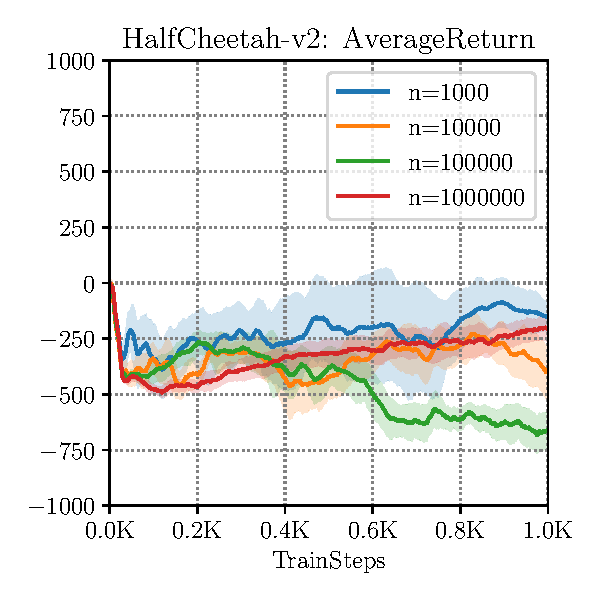
\includegraphics[width=0.45\linewidth]{chapters/bear/images/cheetah_divergence.pdf}
    ~
    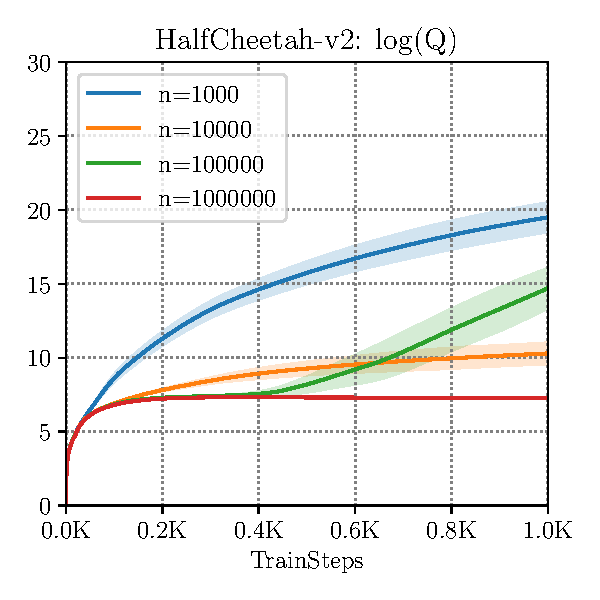
\includegraphics[width=0.45\linewidth]{chapters/bear/images/cheetah_divergence_q_val.pdf}
  \end{center}
 \vspace{-10pt}
 %%SL.5.22: Very important: the y-axes are not labeled right now, and it took me a while to figure out which plot was showing what. What is log(Q)? I guess you're trying to show that the right plot has Bellman error (?), while the left has performance? A couple more things: (1) always put space before ( (you often omit this space) (2) consider a caption like this (once the figures are labeled more clearly): Off-policy learning with SAC on HalfCheetah-v2 for different dataset sizes ($n$). The performance (left) does not correlate with $n$, while the Q-values (right) diverge or saturate at values far from the actual return.
  \caption{ \footnotesize Performance of SAC on HalfCheetah-v2 (return (left) and $\log$ Q-values (right)) with off-policy expert data w.r.t. number of training samples ($n$). Note the large discrepancy between returns (which are negative) and $\log$ Q-values (which have large positive values), which is not solved with additional samples.} 
 \vspace{-15pt}
 \label{fig:divergence}
\end{figure}
Building upon the discoveries presented in Chapter~\ref{chapter:diagnosing}, we have observed that Q-learning methods frequently struggle to learn from static, off-policy data, particularly in high-dimensional tasks. This difficulty is evident in Figure \ref{fig:divergence}. As outlined in the discussion of Chapter~\ref{chapter:diagnosing}, the primary cause of this instability lies in the challenges of handling distributional shift and statistical error. However, a crucial question remains: which factor plays a more significant role in this example? Furthermore, what mechanism underlies the emergence of this instability?

First of all, note that increasing the size of the static dataset does not rectify the problem (compare $n=1M$ vs $n=1000$), suggesting the issue in this setting is largely due to distributional shift. We can understand the source of this instability by examining the form of the Bellman backup. Although minimizing the mean squared Bellman error corresponds to a supervised regression problem, the targets for this regression are themselves derived from the current Q-function estimate. The targets are calculated by maximizing the learned $Q$-values with respect to the action at the next state. However, the $Q$-function estimator is only reliable on inputs from the same distribution as its training set. As a result, na\"{i}vely maximizing the value may evaluate the $\hat{Q}$ estimator on actions that lie far outside of the training distribution, resulting in pathological values that incur large error. We refer to these actions as out-of-distribution (OOD) actions. 

Formally, let $\valerr_k(\bs, \mathbf{a}) = |Q_k(\bs, \mathbf{a}) - Q^*(\bs, \mathbf{a})|$ denote the total error at iteration $k$ of Q-learning, and let $\projerr_k(\bs, \mathbf{a}) = |Q_k(\bs, \mathbf{a}) - \mathcal{B} Q_{k-1}(\bs, \mathbf{a})|$ denote the current Bellman error. Then, we have \mbox{$\valerr_k(\bs, \mathbf{a}) \le \projerr_k(\bs, \mathbf{a}) + \gamma \max_{\mathbf{a}'} \expec_{\bs'}[\valerr_{k-1}(\bs', \mathbf{a}')]$}. In other words, errors from $(\bs', \mathbf{a}')$ are discounted, then accumulated with new errors $\projerr_k(\bs, \mathbf{a})$ from the current iteration. We expect $\projerr_k(\bs, \mathbf{a})$ to be high on OOD states and actions, as errors at these state-actions are never directly minimized while training.

To mitigate bootstrapping error, we can restrict the policy to ensure that it output actions that lie in the support of the training distribution. This is distinct from previous work~\citep{jaques2019way} which implicitly constrains the \emph{distribution} of the learned policy to be close to the behavior policy, similarly to behavioral cloning~\cite{Schaal99isimitation}.
While this is sufficient to ensure that actions lie in the training set with high probability, it is overly restrictive. For example, if the behavior policy is close to uniform, the learned policy will behave randomly, resulting in poor performance, even when the data is sufficient to learn a strong policy (see Figure~\ref{fig:gridworld}
for an illustration). {Formally, this means that a learned policy $\pi(\mathbf{a}| \bs)$ has positive density\textit{ only where} the density of the behaviour policy $\beta(\mathbf{a}|s)$ is more than a threshold (i.e., $\forall \mathbf{a}, \beta(\mathbf{a}|\bs) \leq \varepsilon \implies \pi(\mathbf{a}|\bs) = 0$), instead of a closeness constraint on the value of the density $\pi(\mathbf{a}|\bs)$ and $\beta(\mathbf{a}|\bs)$.}
Our analysis instead reveals a tradeoff between staying within the data distribution and finding a suboptimal solution when the constraint is too restrictive. Our analysis motivates us to restrict the support of the learned policy, but not the probabilities of the actions lying within the support. This avoids evaluating the Q-function estimator on OOD actions, but remains flexible in order to find a performant policy. Our proposed algorithm leverages this insight. 

\vspace{-0.2cm}
\section{Formal Analysis and Distribution-Constrained Backups}
\label{sec:dist_constrained}
\vspace{-0.2cm}
In this section, we define and analyze a backup operator that restricts the set of policies used in the maximization of the Q-function, and we derive performance bounds which depend on the restricted set. This provides motivation for constraining policy support to the data distribution, allowing us to address the issue discussed above. We begin with the definition of a distribution-constrained operator:

\begin{tcolorbox}[colback=blue!6!white,colframe=black,boxsep=0pt,top=3pt,bottom=5pt]
\begin{definition}[Distribution-constrained operators]
Given a set of policies $\Pi$, the distribution-constrained backup operator is defined as:
%\[ \TPi Q(s, a) \coloneqq \expec \big[ R(s, a) + \gamma \expec_{\trans(s' | s, a)}\left[\max_{\pi \in \Pi} \expec_{\pi}[Q(s', a')] \right] \big] \]
\begin{align*}
\TPi Q(\mathbf{s}, \mathbf{a}) \defeq \expec \big[ R(\bs, \mathbf{a}) + \gamma \max_{\pi \in \Pi} \expec_{\trans(\bs' | \bs, \mathbf{a})}\left[V(\bs') \right] \big]
\ \ \ \ \ \ \ \ \ \ \ \ 
V(\bs) \defeq \max_{\pi \in \Pi} \expec_{\pi}[Q(\mathbf{s}, \mathbf{a})]\ \ .
\end{align*}
\end{definition}
\end{tcolorbox}
This backup operator satisfies properties of the standard Bellman backup, such as convergence to a fixed point, as discussed in Appendix~\ref{app:constrained_backup}. To analyze the (sub)optimality of performing this backup under approximation error, we first quantify two sources of error. The first is a \emph{suboptimality bias}. The optimal policy may lie outside the policy constraint set, and thus a suboptimal solution will be found. The second arises from distribution shift between the training distribution and the policies used for backups. This formalizes the notion of OOD actions. %and states.
To capture suboptimality in the final solution, we define a \emph{suboptimality constant}, which measures how far $\pi^*$ is from $\Pi$. 

\begin{definition}[Suboptimality constant]
The suboptimality constant is defined as:
\[ \alpha(\Pi) = \max_{\bs, \mathbf{a}} |\TPi Q^*(\bs, \mathbf{a}) - \backup Q^*(\bs, \mathbf{a})|. \]
\end{definition}
\vspace{-10pt}
Next, we define a concentrability coefficient~\citep{munos2005erroravi}, which quantifies how far the visitation distribution generated by policies from $\Pi$ is  from the training data distribution. This constant captures the degree to which states and actions are out of distribution.
\begin{tcolorbox}[colback=blue!6!white,colframe=black,boxsep=0pt,top=3pt,bottom=5pt]
\begin{assumption}[Concentrability]
Let $\rhoinit$ denote the initial state distribution, and $\mu(\bs, \mathbf{a})$ denote the distribution of the training data over $\mathcal{S} \times \mathcal{A}$, with marginal $\mu(\bs)$ over $\mathcal{S}$. Suppose there exist coefficients $c(k)$ such that for any $\pi_1, ... \pi_k \in \Pi$ and $s \in \mathcal{S}$:
\[
\rhoinit P^{\pi_1}P^{\pi_2}...P^{\pi_k}(s) \le c(k) \mu(\bs),
\]
where $P^{\pi_i}$ is the transition operator on states induced by $\pi_i$.
Then, define the concentrability coefficient $C(\Pi)$ as
\[
C(\Pi) \defeq (1-\gamma)^2\sum_{k=1}^\infty k\gamma^{k-1}c(k).
\] \label{assumption:conc} \end{assumption} 
\end{tcolorbox}
% \vspace{-10pt}
To provide some intuition for $C(\Pi)$, if $\mu$ was generated by a single policy $\pi$, and $\Pi = \{\pi\}$ was a singleton set, then we would have $C(\Pi)=1$, which is the smallest possible value. However, if $\Pi$ contained policies far from $\pi$, the value could be large, potentially infinite if the support of $\Pi$ is not contained in $\pi$. Now, we bound the performance of approximate distribution-constrained Q-iteration:

\begin{tcolorbox}[colback=blue!6!white,colframe=black,boxsep=0pt,top=3pt,bottom=5pt]
\begin{theorem}
\label{thm:avi_bound}
Suppose we run approximate distribution-constrained value iteration with a set constrained backup $\TPi$. Assume that $\delta(\bs,\mathbf{a}) \ge \max_k |Q_k(\bs, \mathbf{a}) - \TPi Q_{k-1}(\bs, \mathbf{a})|$ bounds the Bellman error. Then,
\[\lim_{k \to \infty} \expec_{\rhoinit}[|V^{\pi_k}(\bs) - V^*(\bs)|] \le
\frac{\gamma}{(1-\gamma)^2}\left[ C(\Pi)\expec_\mu[\max_{\pi \in \Pi} \expec_{\pi}[\projerr(\bs, \mathbf{a})]] + \frac{1-\gamma}{\gamma}\alpha(\Pi) \right]
\]
\end{theorem}
\end{tcolorbox}
\begin{proof} See Appendix~\ref{app:error_prop}, Theorem~\ref{thm:avi_bound_proof} \end{proof}
This bound formalizes the tradeoff between keeping policies chosen during backups close to the data (captured by $C(\Pi)$) and keeping the set $\Pi$ large enough to capture well-performing policies (captured by $\alpha(\Pi)$). When we expand the set of policies $\Pi$, we are increasing $C(\Pi)$ but decreasing $\alpha(\Pi)$. An example of this tradeoff, and how a careful choice of $\Pi$ can yield superior results, is given in a tabular gridworld example in Fig.~\ref{fig:gridworld}, where we visualize errors accumulated during distribution-constrained Q-iteration for different choices of $\Pi$. 

Finally, we motivate the use of support sets to construct $\Pi$. We are interested in the case where $\Pi_\epsilon = \{ \pi ~|~ \pi( \mathbf{a} | \bs) = 0 \text{ whenever } \beta( \mathbf{a} | \bs) < \epsilon \}$, where $\beta$ is the behavior policy (i.e., $\Pi$ is the set of policies that have support in the probable regions of the behavior policy). Defining $\Pi_\epsilon$ in this way allows us to bound the concentrability coefficient:

\begin{tcolorbox}[colback=blue!6!white,colframe=black,boxsep=0pt,top=3pt,bottom=5pt]
\begin{theorem}
\label{thm:conc_coeff_bound}
% Assume the data distribution $\mu$ is generated by a policy $\beta$, such that $\mu(s,a) = d_\beta(s,a)$. Let $\mu_\beta(s)$ be the state-visitation marginal for $\beta$. Let us define $\Pi_\epsilon = \{ \pi ~|~ \pi( a | s) = 0 \text{ whenever } \beta( a | s) < \epsilon \}$. Let $\mu_{\Pi}(s)$ be the maximum discounted visitation marginal of a state generated by some sequence of policies $\{\pi_i\}_{i} \in \Pi$ and let $f(\epsilon) \defeq \min_{s \in \mathcal{S}, \mu_\Pi(s) > 0} [\mu(s)]$. Then, Assumption~\ref{assumption:conc} is satisfied for a $C(\Pieps)$ that is bounded as:
% \[
% C(\Pi_\epsilon) \leq C(\beta) \cdot \Big(1 + \frac{\gamma}{(1 - \gamma) f(\epsilon)} (1 - \epsilon)\Big)
% \]
Assume the data distribution $\mu$ is generated by a behavior policy $\beta$. %, such that $\mu(s,a) = d_\beta(s,a)$. 
Let $\mu(\bs)$ be the marginal state distribution under the data distribution. Define $\Pieps = \{ \pi ~|~ \pi( \mathbf{a} | \bs) = 0 \text{ whenever } \beta( \mathbf{a} | \bs) < \epsilon \}$ and let $\mu_\Pieps$ be the highest discounted marginal state distribution starting from the initial state distribution $\rho$ and following policies $\pi \in \Pieps$ at each time step thereafter. Then, there exists a concentrability coefficient $C(\Pieps)$ which is bounded:
\[
C(\Pi_\epsilon) \leq C(\beta) \cdot \Big(1 + \frac{\gamma}{(1 - \gamma) f(\epsilon)} (1 - \epsilon)\Big)
\]
where $f(\epsilon) \defeq \min_{\bs \in \mathcal{S}, \mu_\Pieps(\bs) > 0} [\mu(\bs)] > 0$.
\end{theorem}
\end{tcolorbox}
% \vspace{-10pt}
\begin{proof} See Appendix~\ref{app:error_prop}, Theorem~\ref{thm:conc_coeff_proof} \end{proof}
% \vspace{-10pt}
Qualitatively, $f(\epsilon)$ is the minimum discounted visitation marginal of a state under the behaviour policy if only actions which are more than $\epsilon$ likely are executed in the environment. Thus, using support sets gives us a single lever, $\epsilon$, which simultaneously trades off the value of $C(\Pi)$ and $\alpha(\Pi)$. Not only can we provide theoretical guarantees, we will see in our experiments (Sec.~\ref{sec:experiments}) that constructing $\Pi$ in this way provides a simple and effective method for implementing distribution-constrained algorithms. 

Intuitively, this means we can prevent an increase in overall error in the Q-estimate by selecting policies supported on the support of the training action distribution, which would ensure roughly bounded projection error $\delta_k(\mathbf{s}, \mathbf{a})$ while reducing the suboptimality bias, potentially by a large amount. Bounded error $\delta_k(\bs, \mathbf{a})$ on the support set of the training distribution is a reasonable assumption when using highly expressive function approximators, such as deep networks, especially if we are willing to reweight the transition set~\cite{Schaul2015,fu2019diagnosing}. We further elaborate on this point in Appendix~\ref{app:bearql-more}.

\begin{figure}
    \centering
    \vspace{-0.1in}
    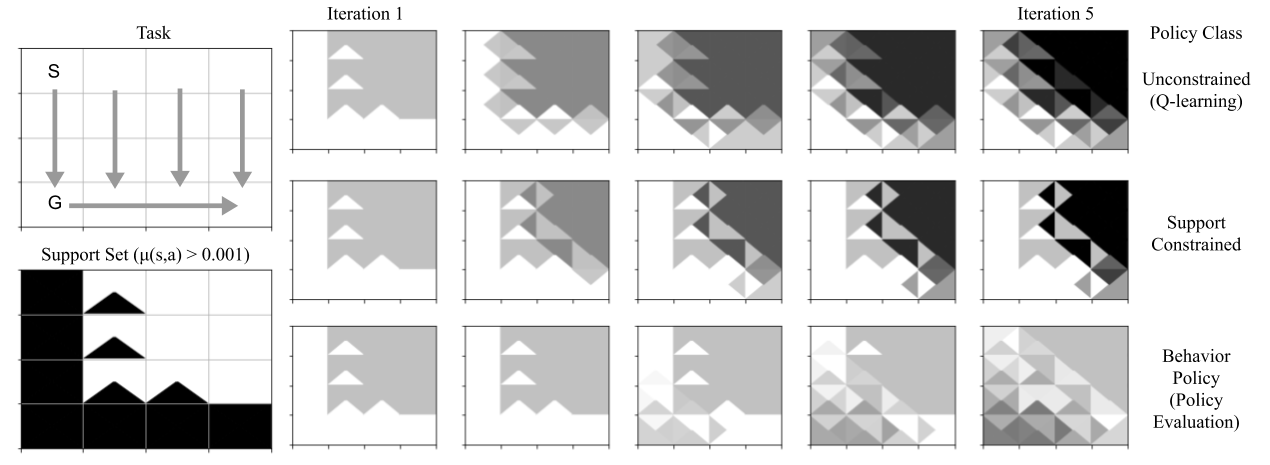
\includegraphics[width=0.9\textwidth]{chapters/bear/images/gridworld}
    \caption{ \footnotesize Visualized error propagation in Q-learning for various choices of the constraint set $\Pi$:
    unconstrained (top row) distribution-constrained (middle),
    and constrained to the behavior policy (policy-evaluation, bottom). Triangles represent Q-values for actions that move in different directions. The task (left) is to reach the bottom-left corner (G) from the top-left (S), but the behaviour policy (visualized as arrows in the task image, support state-action pairs are shown in black on the support set image) travels to the bottom-right with a small amount of $\epsilon$-greedy exploration. Dark values indicate high error, and light values indicate low error. Standard backups propagate large errors from the low-support regions into the high-support regions, leading to high error. Policy evaluation reduces error propagation from low-support regions, but introduces significant suboptimality bias, as the data policy is not optimal. A carefully chosen distribution-constrained backup strikes a balance between these two extremes, by confining error propagation in the low-support region while introducing minimal suboptimality bias.}
    \label{fig:gridworld}
    \vspace{-0.1in}
\end{figure}

% \subsection{Choosing Backup Policies for OOD Action Error Reduction}
% \label{sec:choosing_policies}
% Argument in Sec.~\ref{sec:tradeoff} tells us that, with a careful selection of the policy under which the target value is computed, the overall error of value estimates from the optimal value function $\|V^* - V_k\|$ can be reduced. How should we search for a policy that minimizes the overall error? Our choice is to backup from policies which maintain high-support over the action set of the data.
% %%SL.5.22: I think it's not obvious to readers that "policy for the backup" means the distribution over the actions under which the target value is calculated. -- addressed

% To justify this choice,
% %%SL.5.22: What choice? -- choice of backing up from any policy that maintains high support over data.
% we note that the error analysis relies on being able to quantify $\delta_k(s, a)$ (the per-state-action bellman error) for OOD actions. Outside of the support of the data distribution, it is hard to provide guarantees on $\delta_k$. However, when $a$ lies inside the support of the training distribution for a given state $s$, high-capacity function approximators trained with supervised learning are expected to produce a bounded error, given enough samples.
% %Even if they don't produce bounded error on such in-support inputs, techniques such as Prioritized Replay~\cite{Schaul2016PrioritizedER} can be employed to ensure bounded error on all in-support inputs. 
% %Furthermore, often the quantity of interest is the Bellman error weighted by the inverse density of the behaviour policy~\cite{antos07fitted}, which depends only on the support of the behaviour policy and this error metric is the equal for two policies provided they share the same support.
% Therefore, backing up from all actions that have non-negligible support under the training distribution is sufficient (but not necessary) to prevent error accumulation. Hence, we restrict the set $\Pi$
% %%SL.5.22: Did we define \Pi before? since we cut the set backup operator stuff, now this is much harder to follow. Maybe we can bring it back (but call it something else)?
% of policies used for distribution-constrained backups to the set of policies that are supported on the probable regions of the behaviour policy. That is, $\Pi = \{ \pi | \pi( a | s) = 0 \text{ whenever } \beta( a | s) < \epsilon \}$, where $\beta$ is the behavior policy (i.e., the set of policies that have support in the probable regions of the behavior policy). This means that we are allowed to backup from any action distribution supported over the support of the behaviour policy. Previous work~\cite{fujimoto2018off} restricts the choice of actions to be a distribution close to the behaviour policy. 

%%SL.5.22: I don't really understand what the above paragraph is saying. Read literally, it seems to say "prior work does something similar, and in the worst case we are equally bad." That's not very satisfying. Maybe just delete this paragraph, or rephrase if that's not what you meant?
%Now, explain why this does a good job of balancing the terms. Next, we explain how this bound motivates the use of set-constrained backups to reduce accumulation of bootstrapping error. \TODO{explanation about $\delta1$ goes here} -- addressed -- removed this paragraph


% we need to determine how to formulate the appropriate constraint and how to implement so as to back up only values of policies in $\Pi$.
% %%SL.5.20: Rephrase. In order to develop a practical algorithm based on the set-constrained backup, we need to determine how to formulate the appropriate constraint and how to implement so as to back up only values of policies in $\Pi$.
% Intuitively, we would like $\Pi(s)$ for a particular state $s$ to contain only those policies that permit actions within the support of the dataset distribution. Instead of inferring $\Pi$, we use a notion of divergence between the uniform distribution over the support-set of the current policy and the current policy for optimization.  

% %%SL.5.20: Rephrase. Intuitively, we would like $\Pi(s)$ for a particular state $s$ to contain only those policies that permit actions withi
% In order confidence support set perform the $\max$ on the high-over actions from only these policies, we need to define a tractable objective. Instead of inferring the set of policies $\Pi$ we rather resort to specifying a notion of divergence between the set $\mathcal{A}_\varepsilon^\dataset$ and the current policy, $\operatorname{Divergence}(\mathcal{A}^{\mathcal{D}}_{\varepsilon}(s), \pi)$ thereby fitting the problem of inferring $\Pi$ in an optimization setup.
% %%SL.5.20: I don't really understand the above sentence. Try rewriting it to be clearer?
% Next, we move on to presenting our method, which we call \emph{bootstrap error accumulation reduction} (BEAR).

\vspace{-0.2cm}
\section{Bootstrapping Error Accumulation Reduction (BEAR)}
\label{sec:bear}
\vspace{-0.2cm}

% \vspace{-0.1in}
We now propose a practical actor-critic algorithm (built on the framework of TD3~\cite{fujimoto18addressing} or SAC~\cite{haarnoja2018sac}) that uses distribution-constrained backups to reduce accumulation of bootstrapping error. The key insight is that we can search for a policy with the same support as the training distribution, while preventing accidental error accumulation.
Our algorithm has two main components. Analogous to BCQ~\citep{fujimoto18addressing}, we use $K$ Q-functions and use the minimum Q-value for policy improvement, and design a constraint which will be used for searching over the set of policies $\Pieps$, which share the same support as the behavior policy. Both of these components will appear as modifications of the policy improvement step in actor-critic style algorithms. We also note that policy improvement can be performed with the mean of the K Q-functions, and we found that this scheme works as good in our experiments. 

% n components. Analogous to BBCQ~\citep{fujimoto2018off}, we use two Q-functions and linearly combine their predictions the Q-function for policy improvement, and design a constraint which will be used for searching over the set of policies $\Pieps$, which share the same support as the behaviour policy. Both of these components will appear as modifications of the policy improvement step in actor-critic style algorithms.

We denote the set of Q-functions as: $\hat{Q}_1, \cdots, \hat{Q}_K$.
% compute a conservative estimate of the Q-values: $\frac{1}{K} \sum_{i=1}^K \hat{Q}_i (s, a) - \lambda \sqrt{\operatorname{var}_k \hat{Q}_k(s, a)}$, where $\lambda \in \mathbb{R}^+$ is a hyperparameter. %We use this value as a conservative estimate of the Q-function. This can be derived using Cantelli's inequality. 
Then, the policy is updated to maximize the conservative estimate of the Q-values within $\Pieps$: 
% \vspace{-10pt}
$$ \pi_\phi(\bs) := \max_{\pi \in \Pieps} \expec_{a \sim \pi(\cdot|\bs)} \left[\min_{j=1,..,K} \hat{Q}_j(\bs, \mathbf{a})\right] $$
% \lambda \sqrt{ \operatorname{var_k}\expec_{a \sim \pi(\cdot |s) }[\hat{Q}_k(s, a)]}.$$
% \vspace{-5pt}
% Let $\mathcal{F}_t$ be the sigma-algebra generated by the training procedure until iteration $t$, and let $\operatorname{var}_{t} \hat{Q}(s,a) := \mathbb{E}[(\hat{Q}_t(s, a) - \mathbb{E}[(\hat{Q}_t(s, a) | \mathcal{F}_t))^2|\mathcal{F}_t]$
%%SL.5.20: use mbox. And for clarity, it might be good to indicate what the expectation is over (and use [ instead of ( for E so that parens don't get cluttered). Also, what is up with this (s,a) hanging out at the end? do you mean to put (s,a) inside (after \hat{Q})?
% denote the variance of the Q-function $\hat{Q}_t$, at time $t$ during training. Then, for each state-action pair $(s, a)$, 
% ${Pr (\hat{Q}_t \geq \mathbb{E}(\hat{Q}_t|\mathcal{F}_t) + \sqrt{\frac{(1 - \delta) \operatorname{var}_{t} \hat{Q}_t }{\delta}})  \leq \delta}$
%%SL.5.20: can you state in words what this means for the purpose of this section? also, rhetoric-wise, amybe better state as a theorem (it's kind of obvious, but still) and then after say that this is easy to show via Cantelli's inequality or something?

%%SL.5.20: It's not clear what the concentration bound is actually used for.

 %In the above concentration bound, $\mathbb{E}(\hat{Q}_t|\mathcal{F}_t)$ refers to the true Q-value, which can be obtained given no stochasticity in the procedure.


%%SL.5.20: The logical thread here is broken. What are you doing with set divergence? State the issue first, then th e resolution, else it's hard for the reader to follow.
In practice, the behavior policy $\beta$ is unknown, so we need an approximate way to constrain $\pi$ to $\Pi$. We define a differentiable constraint that approximately constrains $\pi$ to $\Pi$, and then approximately solve the constrained optimization problem via dual gradient descent.  We use the sampled version of maximum mean discrepancy (MMD)~\cite{gretton2012kernel}
%%SL.5.22: Alg names are not capitalized unless they contain proper nouns, put a space after the words and before open paren (I fixed it above, but this issue happens often, please take this comment into account) -- Thanks for pointing this out!
between the unknown behavior policy $\beta$ and the actor $\pi$ because it can be estimated based solely on samples from the distributions. Given samples $x_1, \cdots, x_n \sim P$ and $y_1, \cdots, y_m \sim Q$, the sampled MMD between $P$ and $Q$ is given by:\\
$$\operatorname{MMD}^2(\{x_1, \cdots, x_n\}, \{y_1, \cdots, y_m\}) = \frac{1}{n^2} \sum_{i, i'} k(x_i, x_{i'}) - \frac{2}{nm} \sum_{i, j} k(x_i, y_j) + \frac{1}{m^2} \sum_{j, j'} k(y_j, y_{j'}).
$$
Here, $k(\cdot, \cdot)$ is any universal kernel. In our experiments, we find both Laplacian and Gaussian kernels work well.
%As the $\operatorname{MMD}$ distance does not depend on the density function of either distribution, minimizing it using samples is a reasonable proxy for enforcing that $Q$ lies inside the support of $P$. This is because, 
The expression for MMD does not involve the density of either distribution and it can be optimized directly through samples. Empirically we find that, in the low-intermediate sample regime, the sampled MMD between $P$ and $Q$ is similar to the MMD between a uniform distribution over $P$'s support and $Q$, which makes MMD roughly suited for constraining distributions to a given support set. (See Appendix~\ref{app:mmd} for numerical simulations justifying this approach).

% and hence, we parameterize the set $\mathcal{A}^{\mathcal{D}}_{\varepsilon}(s)$ as a distribution $\pi_{set}(a|s)$ such that $\mathcal{A}(s) := \mathcal{A}^{\pi_{set}}_{\varepsilon}(s) := \{a \in \mathcal{A} | \pi_{set}(a|s) \geq \varepsilon \}$, in other words, $\mathcal{A}(s)$ is the high-confidence support set of the distribution $\pi_{set}$, and we train for a parametric $\pi_{set}$.
%%SL.5.20: I don't actually understand at this point what you are doing. Are you optimizing a neural net that denotes \pi_set? or something else?

% \paragraph{Deriving the update:} Let $\hat{Q}_k$ be the Q-function at the k-th step of the algorithm. Actor-critic Q-learning algorithms maintain a parameterized policy, $\pi_k$ that is updated towards the maximizing the Q-function.
% %-- $\pi_{k+1}(s) := \max_{\pi \in \Delta_{|S|}} E_{a \sim \pi(\cdot|s)} [\hat{Q}_{k}(s, a)]$. 
% In order to reduce the number of moving parts, we let the actor in this case serve both its regular function of maximizing the Q-function while also constraining the action distribution close to $\mathcal{A}^\dataset_\varepsilon$, which is the the task of $\pi_{set}$. We use the bound derived on Q-values to update the policy in the direction of maximizing a conservative estimate of the true Q-value -- $$ \pi_{k+1}(s) := \max_{\pi \in \Delta_{|S|}} E_{a \sim \pi(\cdot|s)} [\hat{Q}_{k}(s, a)] - \lambda \sqrt{ \operatorname{var_k}E_{a \sim \pi(\cdot |s) }[\hat{Q}_k(s, a)]}$$
% %TODO{may want to mention that this amounts to subtracting a constant times the std, which sounds reasonable}
% We still need to account for the problem of specifying support divergence. In order to enforce this constraint, we use a measure of support matching between the training distribution $\Pi$ and the policy $\pi(\cdot|s)$, which we choose to be a sampled version of the Maximum Mean Discrepancy(MMD) Distance between $\Pi$ and the actor $\pi$. Sampled MMD distance between two probability distributions $P$ and $Q$ is given by, $\operatorname{MMD}(P, Q)$, where $x_1, \cdots, x_n \sim P$ and $y_1, \cdots, y_m \sim Q$ is given by:\\
% $$\operatorname{MMD}^2(\{x_1, \cdots, x_n\}, \{y_1, \cdots, y_m\}) = \frac{1}{n^2} \sum_{i, i'} k(x_i, x_{i'}) - \frac{2}{nm} \sum_{i, j} k(x_i, y_j) + \frac{1}{m^2} \sum_{j, j'} k(y_j, y_{j'})
% $$
% When the number of samples $n$ is an intermediate number (4-10), the above sampled objective can also be approximately considered as a distance between a uniform distribution over the high confidence support set of the distribution $P$ and the distribution $Q$ -- therefore, if trained perfectly, $Q$ should have the same support as $P$. That is, $\operatorname{MMD}(P, Q)$ is a reasonable proxy for $\operatorname{MMD}(\mathcal{U}(\mathcal{A}_{\varepsilon}(P)), Q)$. 
% %\TODO{what does it mean MMD between a set and distribution}
% The expression for $\operatorname{MMD}$ does not use the density function of either distribution, thereby making it suited as an approximate way of support matching.

Putting together, the optimization problem in the policy improvement step is
% \vspace{-5pt}
\begin{multline}
    \label{eqn:policy_update}
   \pi_\phi := \max_{\pi \in \Delta_{|S|}} \expec_{\bs \sim \mathcal{D}} \expec_{\mathbf{a} \sim \pi(\cdot|\bs)} \left[\min_{j=1,..,K} \hat{Q}_j(\bs, \mathbf{a})\right] 
%   - \lambda \sqrt{ \operatorname{var_k}\expec_{a \sim \pi(\cdot |s) }[\hat{Q}_k(s, a)]}\\
   \text{~~s.t.~~} \mathbb{E}_{\bs \sim \mathcal{D}} [\operatorname{MMD}(\mathcal{D}(\bs), \pi(\cdot|\bs))] \leq \varepsilon \quad
\end{multline}
where $\varepsilon$ is an approximately chosen threshold. We choose a threshold of $\varepsilon=0.05$ in our experiments. The algorithm is summarized in Algorithm~\ref{algo:bear_ql}. 
% Step 5 of the algorithm performs a stochastic version of the distribution-constrained backup, where Dirac-delta policies $\delta_{a_i}, \cdots, \delta_{a_p},(~\forall~i, \delta_{a_i} \in \Pi)$ are sampled, an expectation of the target Q-value under these Dirac-delta policies is computed and then the maximum value across these policies is backed up as defined by the backup operator. We provide more explanation in Appendix \ref{app:bearql-more}.

\textbf{How does BEAR connect with distribution-constrained backups described in Section 4.1?} Step 5 of the algorithm restricts $\pi_\phi$ to lie in the support of $\beta$. This insight is formally justified in Theorems 4.1 \& 4.2 ($C(\Pi_\varepsilon)$ is bounded). Computing distribution-constrained backup exactly by maximizing over $\pi \in \Pi_\varepsilon$ is intractable in practice. As an approximation, we sample Dirac policies in the support of $\beta$ (Alg 1, Line 5) and perform empirical maximization to compute the backup. As the maximization is performed over a \textit{narrower} set of Dirac policies ($\{ \delta_{\mathbf{a}_i} \} \subseteq \Pi_\varepsilon$), the bound in the above Theorem still holds. Empirically, we show in Section~\ref{sec:experiments} that this approximation is sufficient to outperform previous methods. This connection is briefly discussed in Appendix~\ref{app:bear_dist_constrained}.
% $\operatorname{var}(\hat{Q}_k(s, a)) \approx \frac{1}{M} \sum_{i=1}^{M} (\hat{Q}_{\theta_i, k}(s, a) - \bar{Q}_{\theta, k}(s, a))^2$, where $\bar{Q}_{\theta, k}(s, a) = \frac{1}{M} \sum_{i=1}^{M} \hat{Q}_{\theta_i, k}(s, a)$ is the sample mean of the ensemble. 

%AK.05.15: Note to Sergey: this is the actor-critic version, optional depends on results.
% Another variant of the above approach can be where this single policy improvement step can be decomposed into two decoupled steps -- (1) Learning a policy $\pi_{set}$, whose high-confidence set defines the support set $\mathcal{A}_{\varepsilon}(s)$ at a state $s$, by minimizing the sampling error in $\hat{Q}_k$ and accounting for the deviation from the dataset, and then, (2) Learning to maximize the expected Q-function $\hat{Q}_k$ on this set $\mathcal{A}_{\varepsilon}(s)$, in practice obtained by sampling from $\pi_{set}$. In practice, we found using Equation~\ref{eqn:policy_update} working better than the latter approach and hence, we stick to this formulation for our experiments. The overall algorithm is summarized in Algorithm~\ref{alg:q_learning}, and the actor-critic version is described in Algorithm~\ref{alg:actor_critic}.   
% \vspace{-5pt}
\begin{algorithm}[h]
\small
\caption{Q-learning variant of BEAR (BEAR)}
\label{alg:q_learning}
\begin{algorithmic}[1]
    \State Dataset $\mathcal{D}$, target network rate $\tau$, batch size $N$, sampled actions for MMD $n$, minimum $\lambda$
    \State Initialize Q-ensemble $\{Q_{\theta_i} \}_{i=1}^{K}$, actor $\pi_{\phi}$, multiplier $\alpha$, target networks $\{ Q_{\theta'_i} \}_{i=1}^K$, and a target actor $\pi_{\phi'}$, with $\phi' \leftarrow \phi, \theta'_i \leftarrow \theta_i$
    \ForAll{$t$ in \{1, \dots, N\}}
        \State Sample mini-batch of transitions $(\bs, \mathbf{a}, r, \bs') \sim \mathcal{D}$\\
        \textbf{Q-update:}
            \State Sample $p$ action samples, $\{\mathbf{a}_i \sim \pi_{\phi'}(\cdot|\bs')\}_{i=1}^p$
            \State Define $y(\bs, \mathbf{a}) := \max_{\mathbf{a}_i} [ \lambda \min_{j=1,..,K} Q_{\theta'_j}(\bs', \mathbf{a}_i) + (1 - \lambda) \max_{j=1,..,K} Q_{\theta'_j}(\bs', \mathbf{a}_i)]$
            \State $\forall i, \theta_i \leftarrow \arg \min_{\theta_i} (Q_{\theta_i}(\bs, \mathbf{a}) - (r + \gamma y(\bs, \mathbf{a})))^2$\\
        \textbf{Policy-update:}
        \State Sample actions $\{ \hat{\mathbf{a}}_i \sim \pi_{\phi}(\cdot | \bs) \}_{i=1}^{m}$ and $\{ \mathbf{a}_j \sim \mathcal{D}(\bs)\}_{j=1}^{n}$. % $n$ preferably an intermediate integer(1-10)
        \State Update $\phi$, $\alpha$ by minimizing Equation~\ref{eqn:policy_update} with Lagrange multiplier $\alpha$.
        \State \textbf{Update Target Networks: } $\theta'_i \leftarrow \tau \theta_i + (1 - \tau)\theta'_i$; $\phi' \leftarrow \tau \phi + (1 -\tau) \phi'$ 
    \EndFor
\end{algorithmic}
\label{algo:bear_ql}
\end{algorithm}

In summary, the actor is updated towards maximizing the Q-function while still being constrained to remain in the valid search space defined by $\Pieps$. The Q-function uses actions sampled from the actor to then perform distribution-constrained Q-learning, over a reduced set of policies. {At test time, we sample $p$ actions from $\pi_\phi(\bs)$ and the Q-value maximizing action out of these is executed in the environment.}  %The maximization step in the actor-update empirically helps, but can be coupled with maximization in Step 5. Similar to \cite{fujimoto2018off} we use a soft-minimum to compute target values for updating Q-functions. 
Implementation and other details are present in Appendix \ref{app:bear_additional_details}.
%%SL.5.22: Remember to fill this in.

% \begin{algorithm}[H]
% \small
% \caption{BEAR Actor-Critic}
% \label{alg:actor_critic}
% \begin{algorithmic}[1]
%     \INPUT: Dataset $\mathcal{D}$, target network update rate $\tau$, mini-batch size $N$, sampled actions for MMD $n$, minimum $\lambda$, policy gradient clipping constants $\beta_1, \beta_2; \beta_1 \leq \beta_2$, MMD threshold constant $\varepsilon$
%     \STATE Initialize Q-ensemble $\{Q_{\theta_i} \}_{i=1}^{M}$, actor $\pi_{\phi}$, set-determining policy $\pi_{set}$, Lagrange multiplier $\alpha$, target networks $\{ Q_{\theta'_i} \}_{i=1}^M$, and a target actor $\pi_{\phi'}$, with $\phi' \leftarrow \phi, \theta'_i \leftarrow \theta_i$
%     \FOR{$t$ in \{1, \dots, N\}}
%         \STATE Sample mini-batch of transitions $(s, a, r, s') \sim \mathcal{D}$\\
%         \textbf{Q-update:}
%             \STATE Sample $m$ action samples, $\{a_i \sim \pi_{\phi'}(\cdot|s')\}_{i=1}^n$
%             \STATE Define $y = \frac{1}{m} \sum_{a_i} [ \lambda \min_{j=1,..,M} Q_{\theta'_j}(s', a_i) + (1 - \lambda) \max_{j=1,..,M} Q_{\theta'_j}(s', a_i)]$
%             \STATE $\forall i, \theta_i \leftarrow \arg \min_{\theta_i} (Q_{\theta_i}(s, a) - (r + \gamma y))^2$\\
%         \textbf{Set-update and Actor-update:}
%         \STATE Sample actions $A_1(s) \equiv \{ \hat{a}_i \sim \pi_{set}(\cdot | s) \}_{i=1}^{m}$ and $A_2(s) \equiv \{ a_j \sim \mathcal{D}(s)\}_{j=1}^{n}$, $n << m$
%         \STATE Update $\pi_{set}, \alpha$: $$ \pi_{set}, \alpha \leftarrow \arg \min_{\pi_{set}} \max_{\alpha \geq 0} \sqrt{\frac{(1 - \delta) \operatorname{var_k}E_{a \sim \pi_{set}(\cdot |s) }[\hat{Q}_k(s, a)]}{\delta}} + \alpha \mathbb{E}_{s \sim \mathcal{D}} ([\operatorname{MMD}(A_1, A_2)] -  \varepsilon) $$
%         \STATE Update $\phi$ using Importance Sampled Policy Gradient: 
%         $$ \pi_{\phi} \leftarrow  \max_{\pi_{\phi}} \mathbb{E}_{s \sim \mathcal{D}} \mathbb{E}_{a \sim \pi_{set}(\cdot|s)} \Big( \Big[ \frac{\pi_\phi(a|s)}{\pi_{set}(a|s)} \Big]_{\beta_1}^{\beta_2} Q(s, a) \Big)$$
%         \STATE \textbf{Update Target Networks: } $\theta'_i \leftarrow \tau \theta_i + (1 - \tau)\theta'_i$; $\phi' \leftarrow \tau \phi + (1 -\tau) \phi'$ 
%     \ENDFOR
% \end{algorithmic}
% \end{algorithm}


% Let $\bar{Q}(\cdot, \cdot)$ be the delayed target network, and $Q(\cdot, \cdot)$ be the current Q-function. Define $d_i$ be the the TD error for the $i^{th}$ datapoint.
% $$
% d_{i}(Q ; \bar{Q}, \pi)=R_{t}+\gamma \bar{Q}\left(s'_{i}, \pi_{set} \left(s'_i\right)\right)-Q\left(s_{i}, a_{i}\right)

% $$
% Further we define the empirical loss function by
% $$
% \hat{L}_{N}(Q ; \bar{Q}, \pi)=\frac{1}{N} \sum_{t=1}^{N} \frac{d_{t}^{2}(Q ; \bar{Q}, \pi_{set})}{\lambda(\mathcal{A})}
% $$
% where normalization $\lambda{\mathcal{A}}$ is introduced for mathematical convenience. Then, each policy evaluation step can be written as:  

% If we solely backup from actions present in our dataset, there is no way the algorithm can perform better than the policy that collected the data. The capacity of Q-learning and other ADP algorithms to ``stitch'' together performant sub-trajectories is lost. Hence, our method does allow the agent to backup from actions that occur outside the dataset, while still being constrained to not go farther away from the support of $\mathcal{D}$. In principle, a measure of distance from a given dataset can only be obtained using Bayesian Approaches (?). In practice, we use the variance of the ensemble as a measure to approximately quantify closeness to the support set. Our overall approach is described in the next paragraph.




% Our problem setting does not allow any interaction with the environment, and only lets us use the dataset $\mathcal{D}$. Since we see a limited subset of state-action pairs from the environment, the expected estimate of the Q-function conditioned on all training history in our case, $\mathbb{E}(\hat{Q}|\mathcal{F}_t)$, is biased. \TODO{aviral: finish this argument} 

% We train an ensemble of $N$ parametric Q-functions, $Q_{\theta_1}, \cdots, Q_{\theta_N}$ by using bootstrap masks on the data points of the dataset $\mathcal{D}$. This is done to simulate epistemic variance. To make sure that the actions chosen for backing up Q-functions are valid, we learn a set selection policy, $\pi_{set}$ -- a policy that can provide high densities to actions that don't propagate errors.   
% \section{Experimental Evaluation}
\label{sec:experiments}
In our experiments, we study how BEAR performs when learning from static offline data on a variety of continuous control benchmark tasks. We evaluate our algorithm in three settings: when the dataset $\dataset$ is generated by \textbf{(1)} a completely random behavior policy, \textbf{(2)} a partially trained, medium scoring policy, and \textbf{(3)} an optimal policy. Condition \textbf{(2)} is of particular interest, as it captures many common use-cases in practice, such as learning from imperfect demonstration data (e.g., of the sort that are commonly available for autonomous driving~\cite{DBLP:conf/iclr/GaoXLYLD18}), or reusing previously collected experience during off-policy RL. We compare our method to several prior methods: a baseline actor-critic algorithm (TD3), the BCQ  algorithm~\citep{fujimoto2018off}, which aims to address a similar problem, as discussed in Section~\ref{sec:Problem Description}, KL-control~\citep{jacques19way} (which solves a KL-penalized RL problem similarly to maximum entropy RL), a static version of DQfD~\citep{hester2018dqfd} (where a constraint to upweight Q-values of state-action pairs observed in the dataset is added as an auxiliary loss on top a regular actor-critic algorithm), and a behavior cloning (BC) baseline, which simply imitates the data distribution. This serves to measure whether each method actually performs effective RL, or simply copies the data. We report the average evaluation return over 5 seeds of the policy given by the learned algorithm, in the form of a learning curve as a function of number of gradient steps taken by the algorithm. These samples are only collected for evaluation, and are not used for training.

\subsection{Performance on Medium-Quality Data}

We first discuss the evaluation of condition with ``mediocre'' data \textbf{(2)}, as this condition resembles the settings where we expect training on offline data to be most useful. We collected one million transitions from a partially trained policy, so as to simulate imperfect demonstration data or data from a mediocre prior policy.
In this scenario, we found that BEAR consistently outperforms BCQ~\cite{fujimoto2018off} and a na\"ive off-policy RL baseline (TD3) (by large margins), as shown in Figure~\ref{fig:mediocre}. This scenario is the most relevant from an application point of view, as access to optimal data may not be feasible, and random data might have inadequate exploration to efficient learn a good policy. We also evaluate the accuracy with which the learned Q-functions predict actual policy returns. These trends are provided in Appendix~\ref{app:q_vs_mc}. 
% Note that the performance of BCQ often tracks the performance of the BC baseline, suggesting that BCQ primarily imitates the data. 
Our KL-control baseline uses automatic temperature tuning~\citep{haarnoja2018sac}. We find that KL-control usually performs similar or worse to BC, whereas DQfD tends to diverge, and often exhibits a huge variance across different runs (for example, HalfCheetah-v2 environment).  

\begin{figure}
    \centering
    \begin{subfigure}[t]{0.23\textwidth}
        \centering
        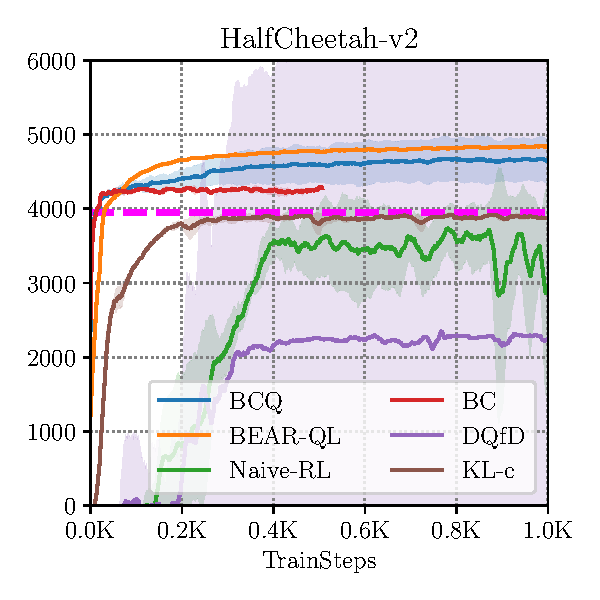
\includegraphics[width=0.99\linewidth]{chapters/bear/images/images_camera_ready/cheetah_mediocre_camera_ready.pdf}
    \end{subfigure}
    \begin{subfigure}[t]{0.23\textwidth}
        \centering
        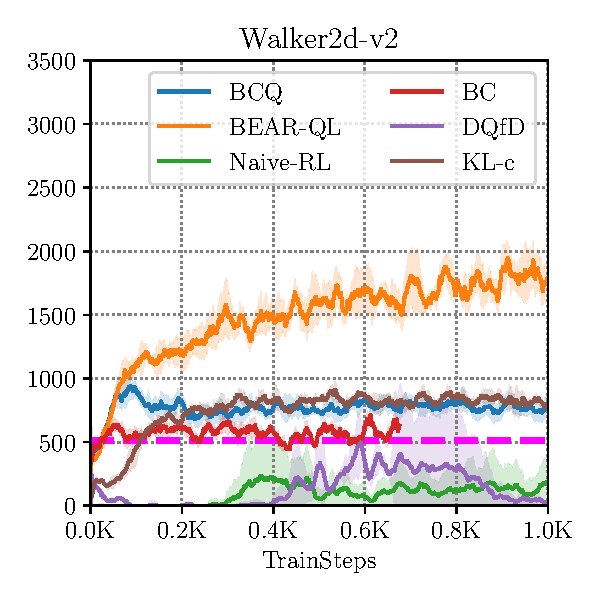
\includegraphics[width=0.99\linewidth]{chapters/bear/images/images_camera_ready/walker_mediocre_camera_ready.pdf}
        % \caption{}
    \end{subfigure}
    ~
    \begin{subfigure}[t]{0.23\textwidth}
        \centering
        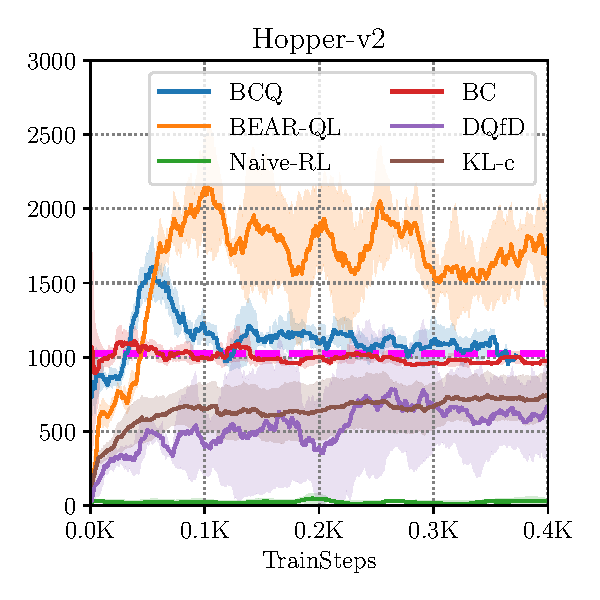
\includegraphics[width=0.99\linewidth]{chapters/bear/images/images_camera_ready/hopper_mediocre_camera_ready.pdf}
        % \caption{}
    \end{subfigure}
    ~
    \begin{subfigure}[t]{0.23\textwidth}
        \centering
        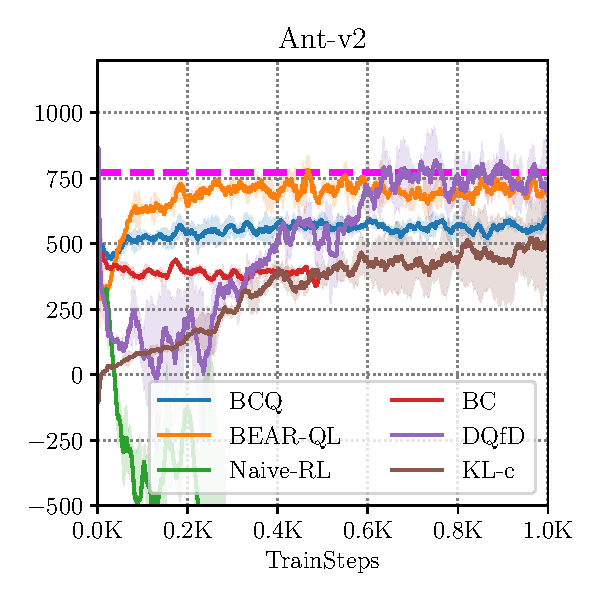
\includegraphics[width=0.99\linewidth]{chapters/bear/images/images_camera_ready/ant_mediocre_camera_ready.pdf}
        % \caption{}
    \end{subfigure}
    \caption{\label{fig:mediocre} \footnotesize Average performance of BEAR, BCQ, Na\"ive RL and BC on medium-quality data averaged over 5 seeds. BEAR outperforms both BCQ and Na\"ive RL. Average return over the training data is indicated by the magenta line. One step on the x-axis corresponds to 1000 gradient steps.}
\end{figure}

% \begin{figure*}[t!]
%     \centering
%     \vspace{-0.05in}
%     \begin{subfigure}[t]{0.23\textwidth}
%         \centering
%         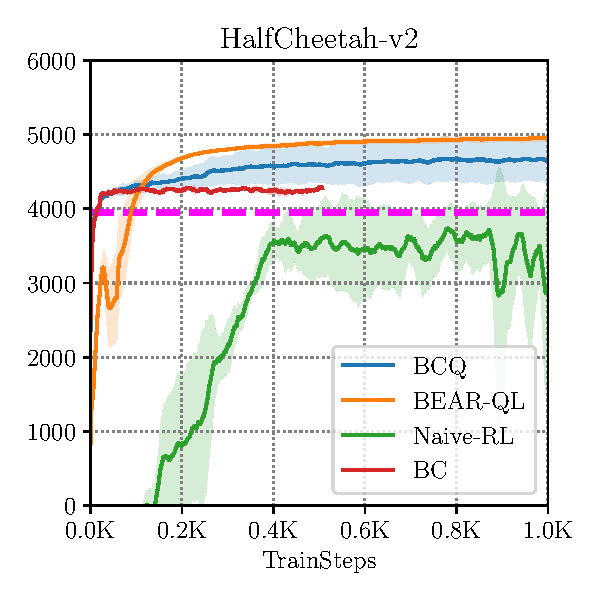
\includegraphics[width=0.99\linewidth]{chapters/bear/images/cheetah_mediocre.pdf}
%     \end{subfigure}
%     \begin{subfigure}[t]{0.23\textwidth}
%         \centering
%         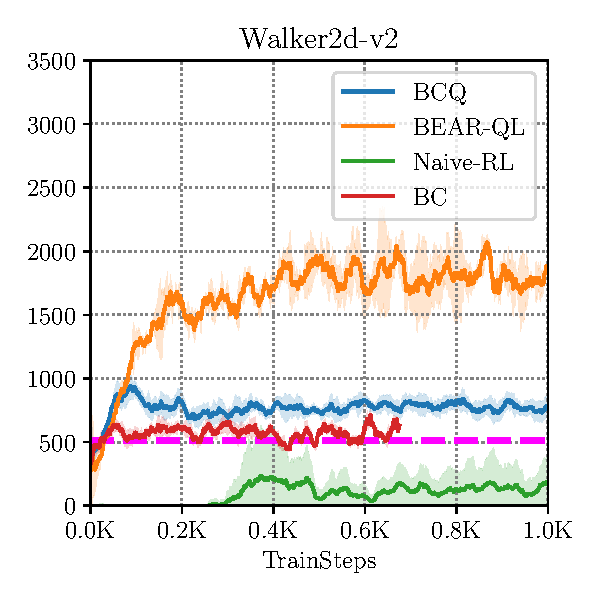
\includegraphics[width=0.99\linewidth]{chapters/bear/images/walker_mediocre_final_again.pdf}
%         % \caption{}
%     \end{subfigure}
%     ~
%     \begin{subfigure}[t]{0.23\textwidth}
%         \centering
%         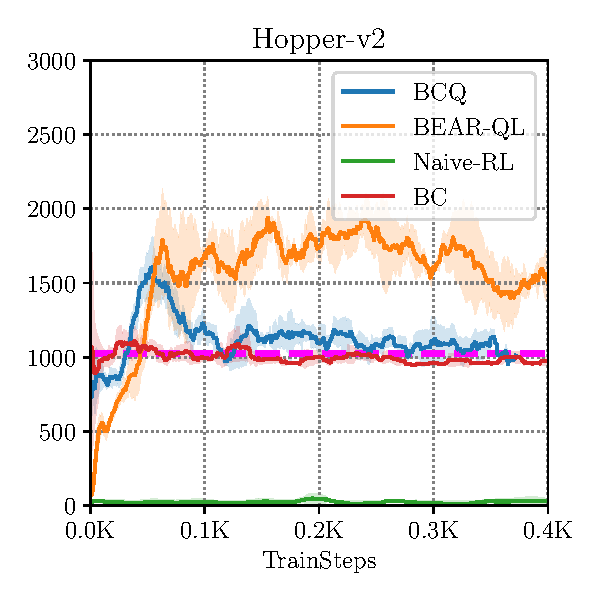
\includegraphics[width=0.99\linewidth]{chapters/bear/images/hopper_mediocre_final_new.pdf}
%         % \caption{}
%     \end{subfigure}
%     ~
%     \begin{subfigure}[t]{0.23\textwidth}
%         \centering
%         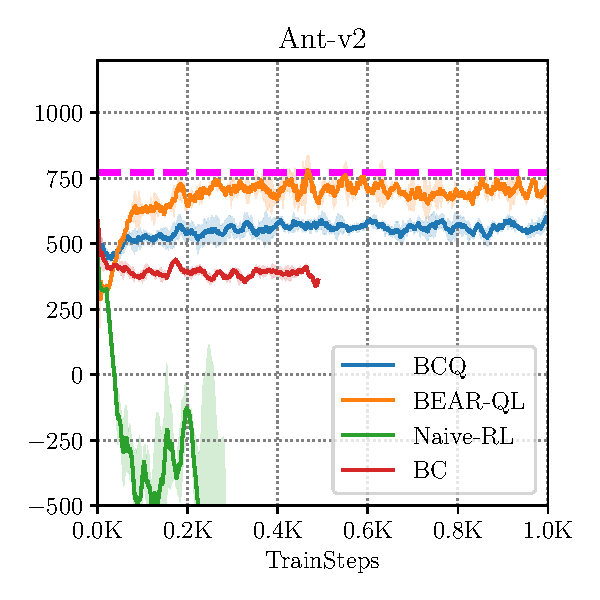
\includegraphics[width=0.99\linewidth]{chapters/bear/images/ant_mediocre_final.pdf}
%         % \caption{}
%     \end{subfigure}
%     \caption{ \footnotesize Average performance of BEAR, BCQ, Na\"ive RL and BC on medium-quality data averaged over 5 seeds. BEAR outperforms both BCQ and Na\"ive RL. Average return over the training data is indicated by the magenta line. One step on the x-axis corresponds to 1000 gradient steps.}
%     \label{fig:mediocre}
%     \vspace{-0.1in}
% \end{figure*}

% \vspace{-5pt}
\subsection{Performance on Random and Optimal Datasets}
In Figure~\ref{fig:optimal_random}, we show the performance of each method when trained on data from a random policy (top) and a near-optimal policy (bottom). In both cases, our method BEAR achieves good results, consistently exceeding the average dataset return on random data, and matching the optimal policy return on optimal data. Na\"{i}ve RL also often does well on random data. For a random data policy, all actions are in-distribution, since they all have equal probability. This is consistent with our hypothesis that OOD actions are one of the main sources of error in off-policy learning on static datasets. The prior BCQ method~\cite{fujimoto2018off} performs well on optimal data but performs poorly on random data, where the constraint is too strict. These results show that BEAR is more robust to the dataset composition, and can learn consistently in a variety of settings. We find that KL-control and DQfD can be unstable in these settings.  

{Finally, in Figure \ref{fig:humanoid}, we  show that BEAR outperforms other considered prior methods in the challenging Humanoid-v2 environment as well, in two cases -- Medium-quality data and random data.}

\begin{figure}
        \centering
        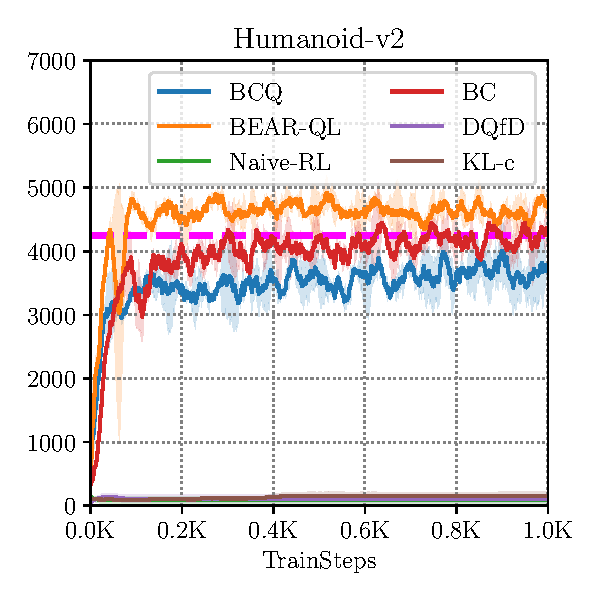
\includegraphics[width=0.4\linewidth]{chapters/bear/images/images_camera_ready/humanoid_mediocre_camera_ready.pdf}
       ~
        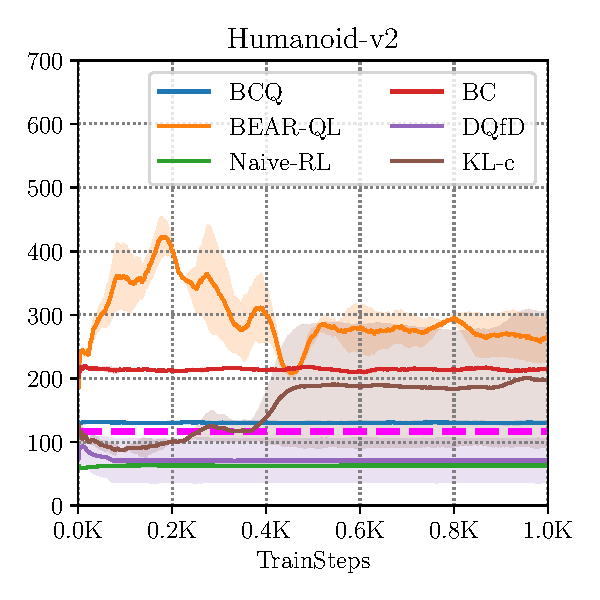
\includegraphics[width=0.4\linewidth]{chapters/bear/images/images_camera_ready/humanoid_random_camera_ready.pdf}
      \caption{\label{fig:humanoid} \footnotesize Performance of BEAR, BCQ, Na\"ive RL and BC on medium-quality (left) and random (right) data in the Humanoid-v2 environment. Note that BEAR outperforms prior methods.}
\end{figure}

%With random data, BCQ is expected to not perform well, as it constrains actions to the actions seen in the dataset at a particular state. On the other hand, a na\"ive off-policy RL algorithm is expected to perform well in these settings. In Figure~\ref{fig:optimal_random}, we show that BEAR outperforms \cite{fujimoto2018off} drastically while still performing comparable to the na\"ive RL algorithm in HalfCheetah-v2, and Hopper-v2, and outperforming it on Walker2d-v2 and Ant-v2 tasks. On optimal data, as the suboptimality bias is small, the best solution is to imitate the behavior policy. BEAR learns to imitate the behavior policy, and maintains stably there. In this setting, na\"ive-RL algorithm fails to learn (and mostly converges to the minimum possible reward, that can be obtained in the environment). Overall, BEAR is robust to the dataset composition, and can consistently perform in all settings -- mediocre, random and optimal data. Figure~\ref{fig:optimal_random} summarizes the average evaluation return of the learned policy as a function of training steps.

% show that DQNs are empirically less stable than off-policy actor critic algorithms(TD3). In all cases, note that BCQ~\cite{fujimoto18addressing} often ends up imitating the baseline, which explains the reason for poor performance on random data, and fast convergence to optimal performance on optimal data. However, the versatility of BEAR demonstrates its use as a practical algorithm irrespective of the quality of the dataset $\dataset$. We also examine the amount of deviation from the true MC-returns of the actor and the learned estimate of the Q-value, which again suggests that BEAR can learn reliable estimates of Q-values without excessive overestimation as observed in TD3, while achieving better expected return performance over BCQ. \TODO{Q vs MC figure left}

\begin{figure}
    \centering
    \begin{subfigure}[t]{0.23\textwidth}
        \centering
        % 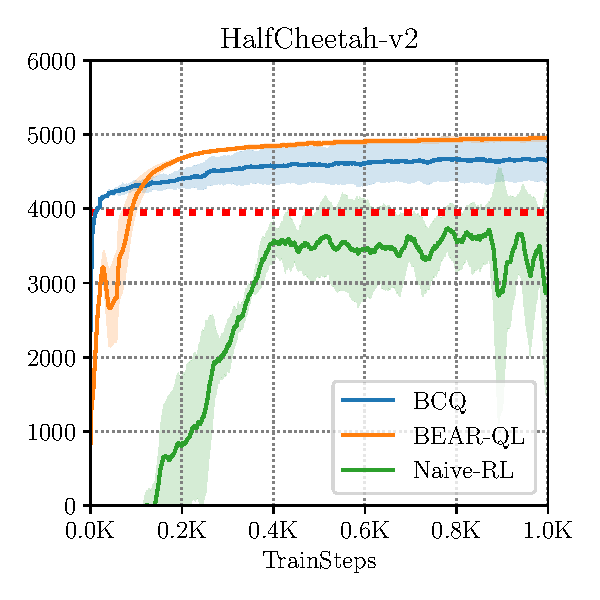
\includegraphics[width=0.99\linewidth]{chapters/bear/images/cheetah_mediocre_final.pdf}
        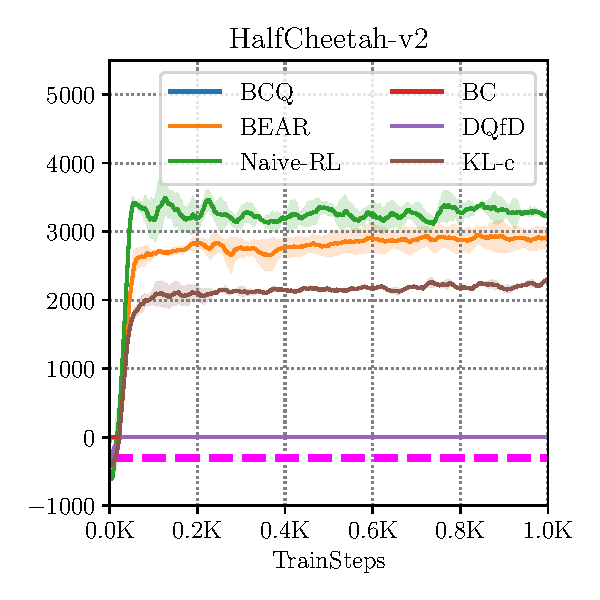
\includegraphics[width=0.99\linewidth]{chapters/bear/images/images_camera_ready/cheetah_random_final_camera_ready.pdf}
        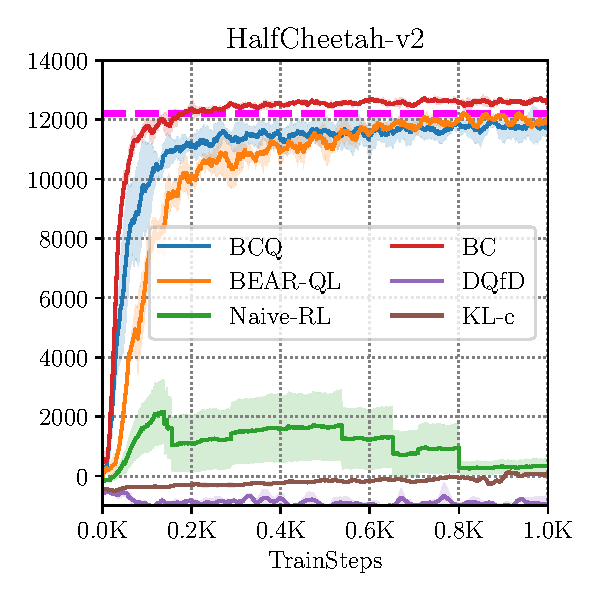
\includegraphics[width=0.99\linewidth]{chapters/bear/images/images_camera_ready/cheetah_optimal_camera_ready_new.pdf}
        % \caption{}
    \end{subfigure}%
    ~ 
    \begin{subfigure}[t]{0.23\textwidth}
        \centering
        % 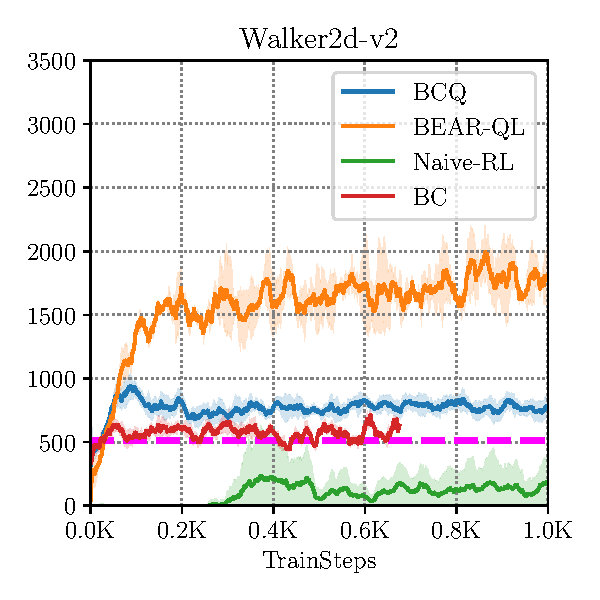
\includegraphics[width=0.99\linewidth]{chapters/bear/images/walker_mediocre_final.pdf}
        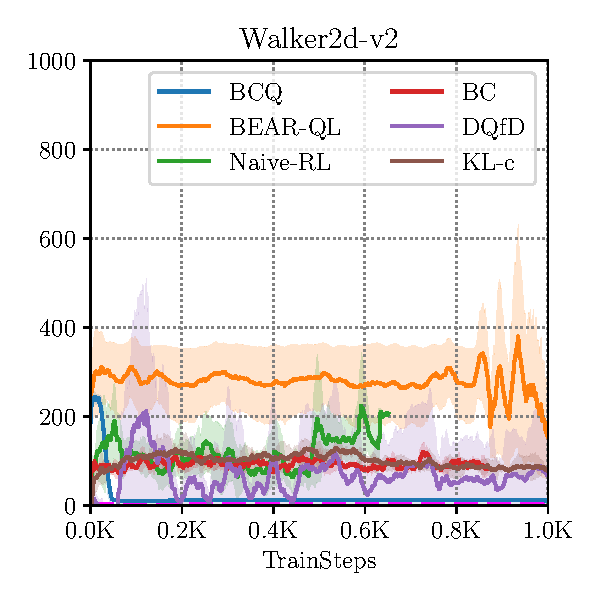
\includegraphics[width=0.99\linewidth]{chapters/bear/images/images_camera_ready/walker_random_camera_ready.pdf}
        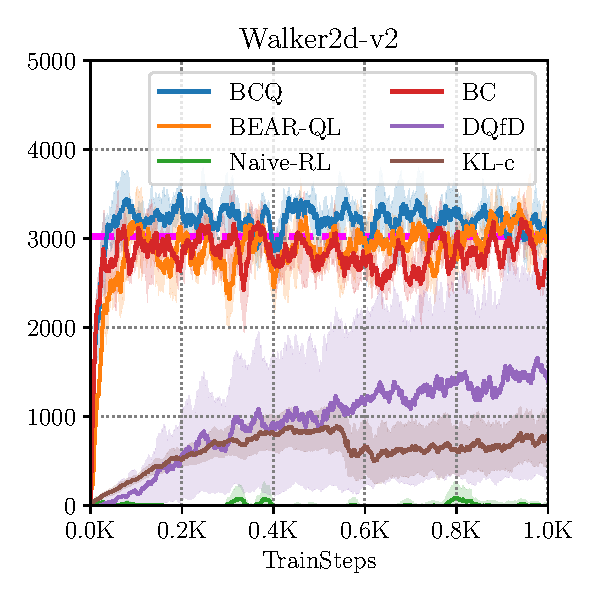
\includegraphics[width=0.99\linewidth]{chapters/bear/images/images_camera_ready/walker_optimal_camera_ready.pdf}
        % \caption{}
    \end{subfigure}
    ~
    \begin{subfigure}[t]{0.23\textwidth}
        \centering
        % 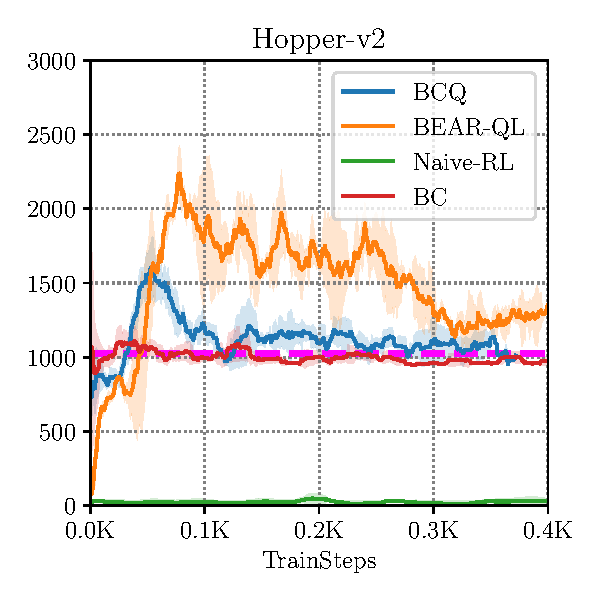
\includegraphics[width=0.99\linewidth]{chapters/bear/images/hopper_mediocre_final.pdf}
        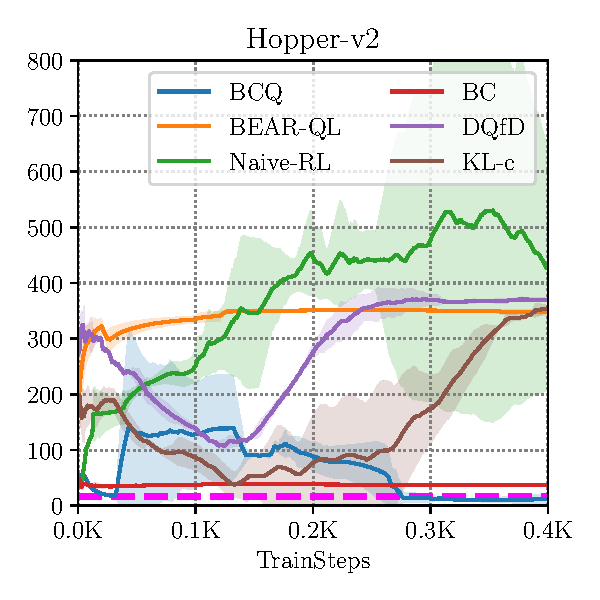
\includegraphics[width=0.99\linewidth]{chapters/bear/images/images_camera_ready/hopper_random_camera_ready.pdf}
        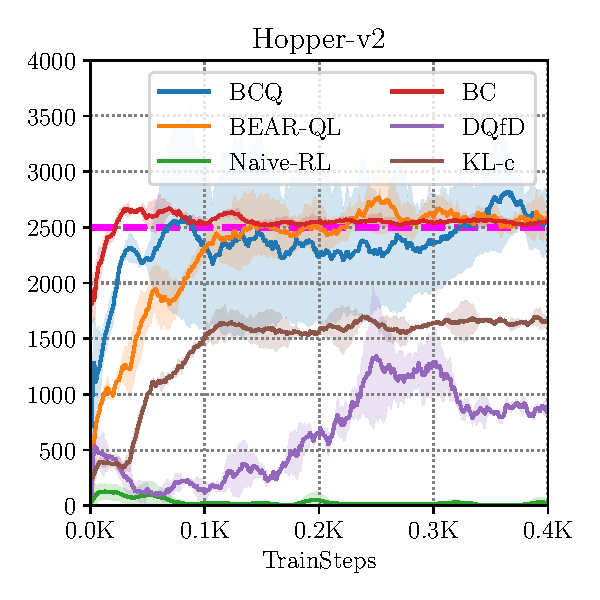
\includegraphics[width=0.99\linewidth]{chapters/bear/images/images_camera_ready/hopper_optimal_camera_ready.pdf}
        % \caption{}
    \end{subfigure}
    ~
    \begin{subfigure}[t]{0.23\textwidth}
        \centering
        % 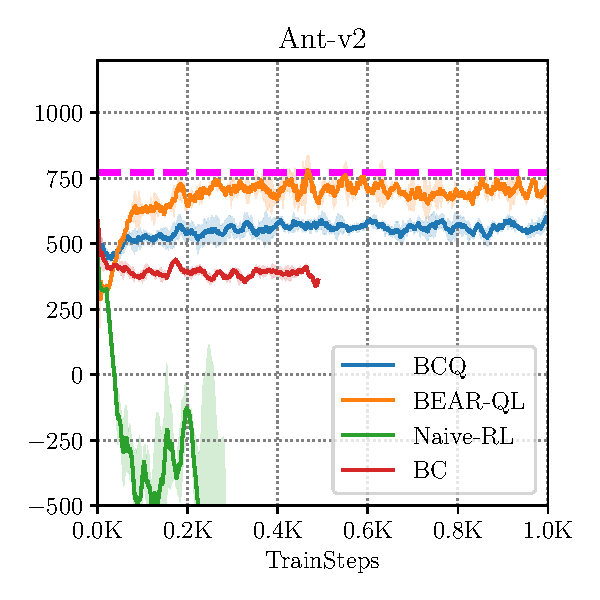
\includegraphics[width=0.99\linewidth]{chapters/bear/images/ant_mediocre_final.pdf}
        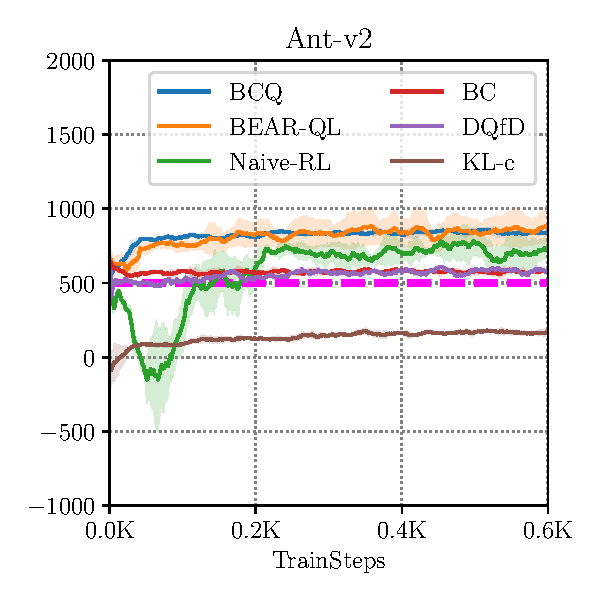
\includegraphics[width=0.99\linewidth]{chapters/bear/images/images_camera_ready/ant_random_camera_ready.pdf}
        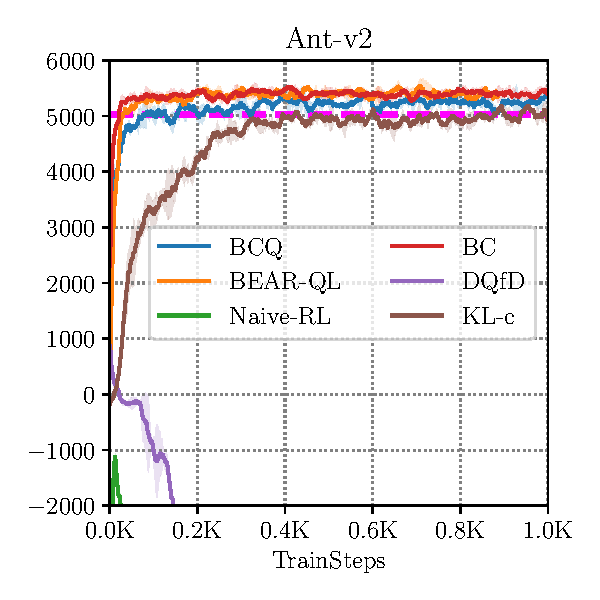
\includegraphics[width=0.99\linewidth]{chapters/bear/images/images_camera_ready/ant_optimal_camera_ready.pdf}
        % \caption{}
    \end{subfigure}
    \caption{\label{fig:optimal_random} \footnotesize Average performance of BEAR, BCQ, Na\"ive RL and BC on random data (top row) and optimal data (bottom row) over 5 seeds. BEAR is the only algorithm capable of learning in both scenarios. Na\"{i}ve RL cannot handle optimal data, since it does not illustrate mistakes, and BCQ favors a behavioral cloning strategy (performs quite close to behavior cloning in most cases), causing it to fail on random data. Average return over the training dataset is indicated by the dashed magenta line.}
\end{figure}

% \begin{figure*}[t!]
% \vspace{-0.1in}
%     \centering
%     \begin{subfigure}[t]{0.23\textwidth}
%         \centering
%         % 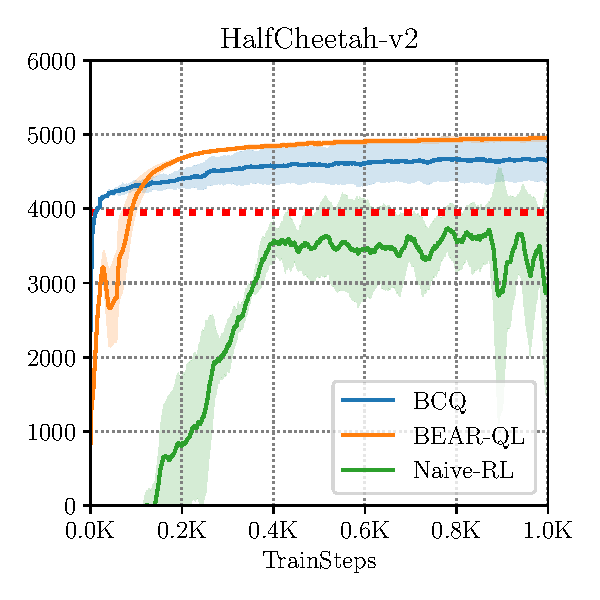
\includegraphics[width=0.99\linewidth]{chapters/bear/images/cheetah_mediocre_final.pdf}
%         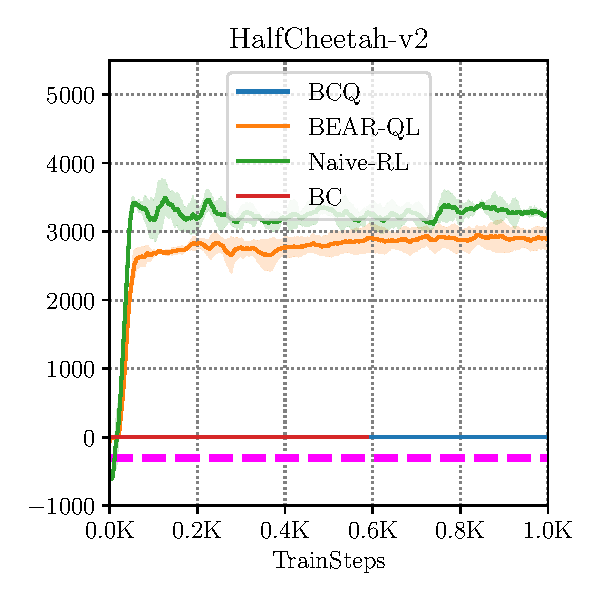
\includegraphics[width=0.99\linewidth]{chapters/bear/images/cheetah_random_final.pdf}
%         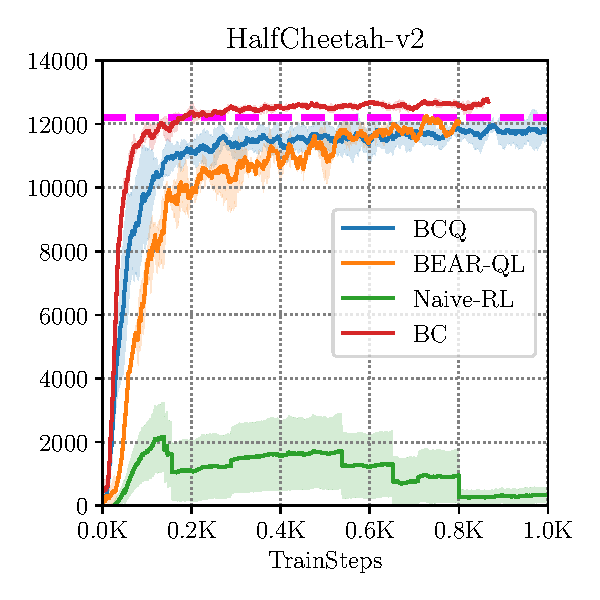
\includegraphics[width=0.99\linewidth]{chapters/bear/images/cheetah_optimal_final.pdf}
%         % \caption{}
%     \end{subfigure}%
%     ~ 
%     \begin{subfigure}[t]{0.23\textwidth}
%         \centering
%         % 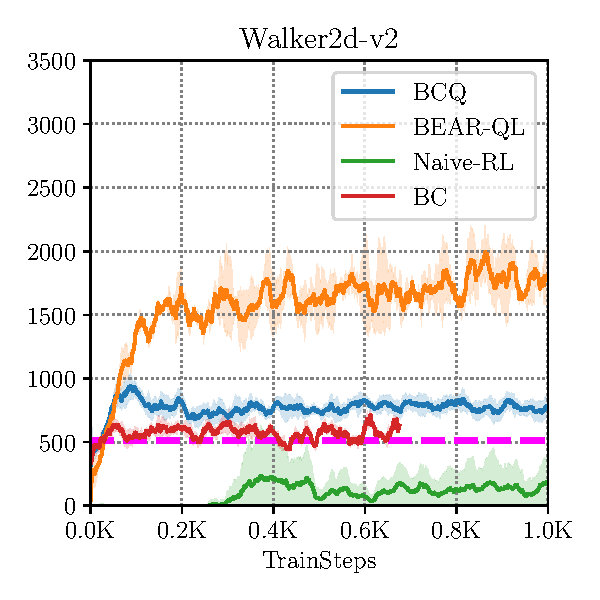
\includegraphics[width=0.99\linewidth]{chapters/bear/images/walker_mediocre_final.pdf}
%         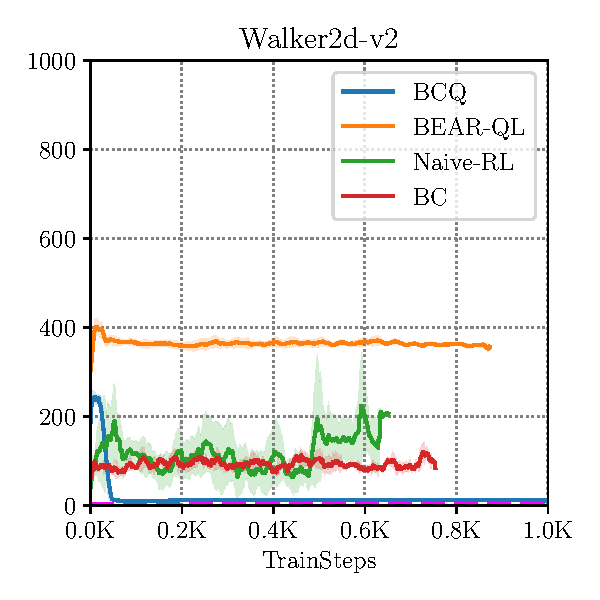
\includegraphics[width=0.99\linewidth]{chapters/bear/images/walker_random_final.pdf}
%         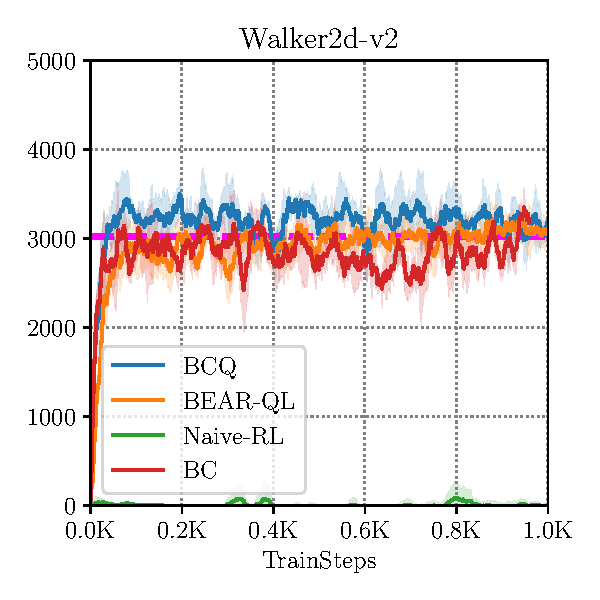
\includegraphics[width=0.99\linewidth]{chapters/bear/images/walker_optimal_final.pdf}
%         % \caption{}
%     \end{subfigure}
%     ~
%     \begin{subfigure}[t]{0.23\textwidth}
%         \centering
%         % 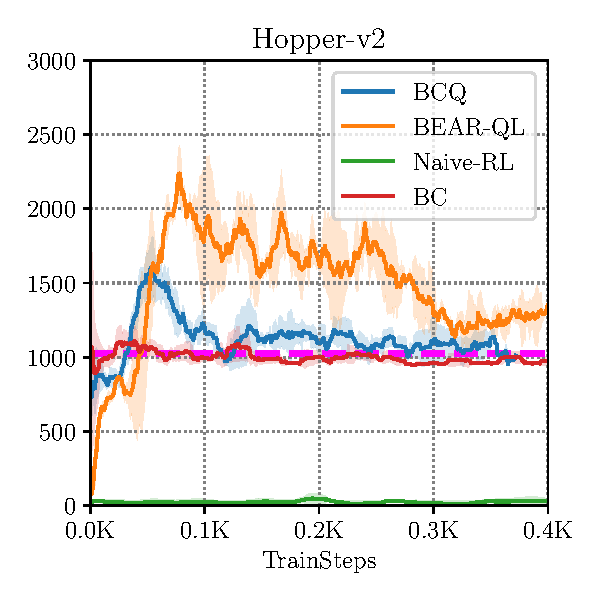
\includegraphics[width=0.99\linewidth]{chapters/bear/images/hopper_mediocre_final.pdf}
%         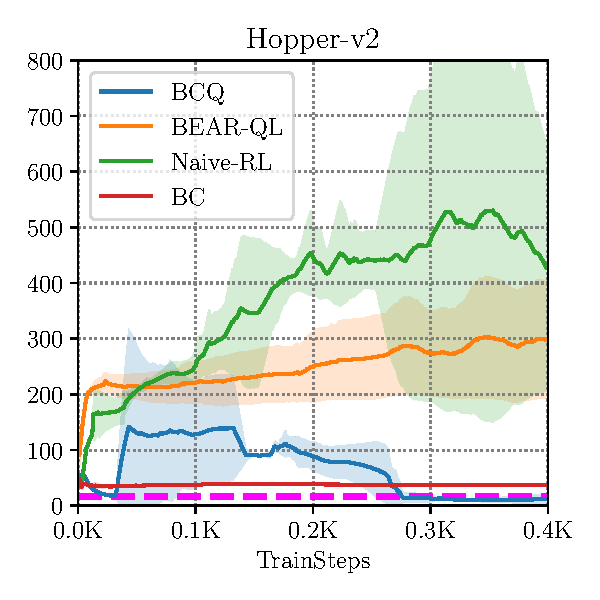
\includegraphics[width=0.99\linewidth]{chapters/bear/images/hopper_random_final.pdf}
%         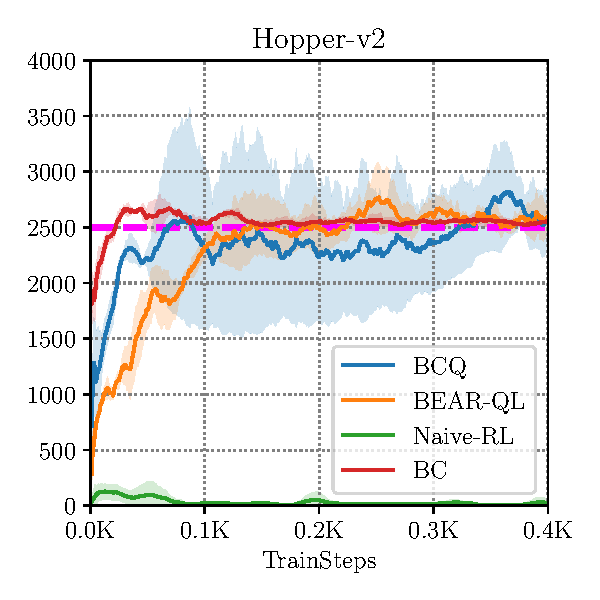
\includegraphics[width=0.99\linewidth]{chapters/bear/images/hopper_optimal_final.pdf}
%         % \caption{}
%     \end{subfigure}
%     ~
%     \begin{subfigure}[t]{0.23\textwidth}
%         \centering
%         % 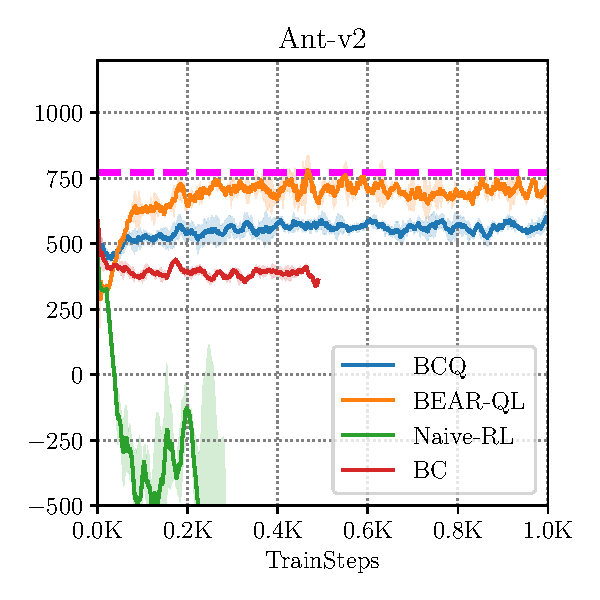
\includegraphics[width=0.99\linewidth]{chapters/bear/images/ant_mediocre_final.pdf}
%         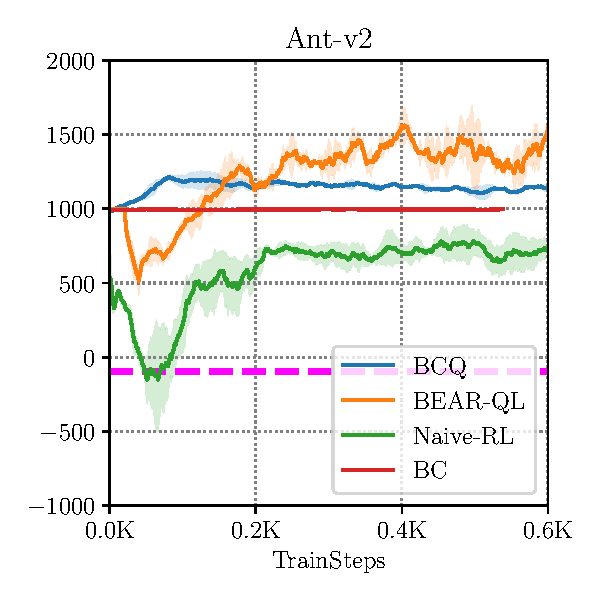
\includegraphics[width=0.99\linewidth]{chapters/bear/images/ant_random_final.pdf}
%         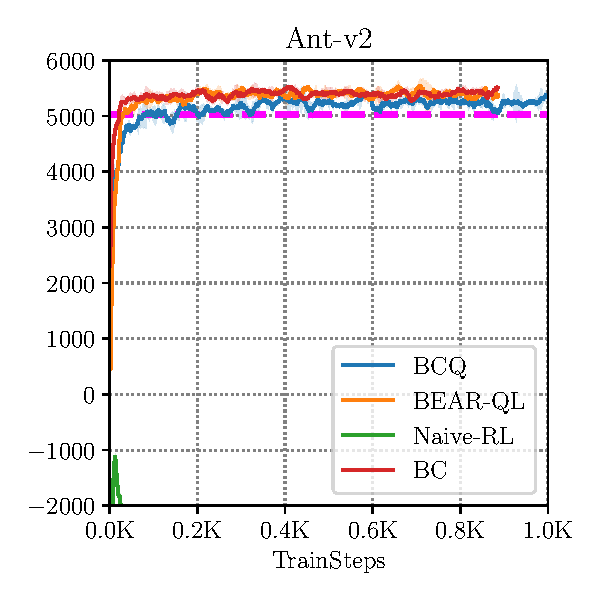
\includegraphics[width=0.99\linewidth]{chapters/bear/images/ant_optimal_final.pdf}
%         % \caption{}
%     \end{subfigure}
%     \caption{\footnotesize Average performance of BEAR, BCQ, Na\"ive RL and BC on random data (top row) and optimal data (bottom row) over 5 seeds. BEAR is the only algorithm capable of learning in both scenarios. Na\"{i}ve RL cannot handle optimal data, since it does not illustrate mistakes, and BCQ favors a behavioral cloning strategy (performs quite close to behavior cloning in most cases), causing it to fail on random data. Average return over the training dataset is indicated by the dashed magenta line.}
%     \label{fig:optimal_random}
%     \vspace{-0.1in}
% \end{figure*}

% \begin{figure*}[t!]
%     \centering
%     \begin{subfigure}[t]{0.31\textwidth}
%         \centering
%         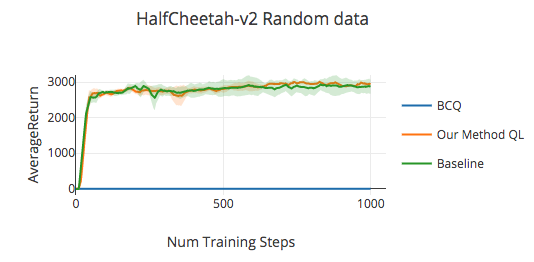
\includegraphics[width=0.99\linewidth]{chapters/bear/images/random_halfcheetah.png}
%         \caption{ }
%     \end{subfigure}%
%     ~ 
%     \begin{subfigure}[t]{0.31\textwidth}
%         \centering
%         \includegraphics[width=0.99\linewidth]{chapters/bear/images/mediocre_walker.png}
%         \caption{ }
%     \end{subfigure}
%     ~
%     \begin{subfigure}[t]{0.31\textwidth}
%         \centering
%         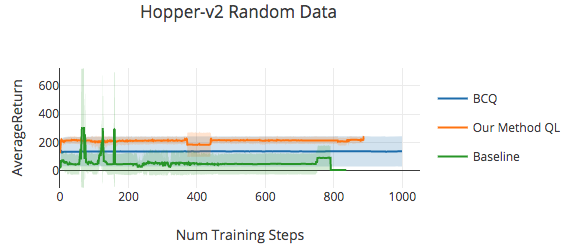
\includegraphics[width=0.99\linewidth]{chapters/bear/images/random_hopper.png}
%         \caption{ }
%     \end{subfigure}
%     \caption{Random Data}
% \end{figure*}

% \begin{figure*}[t!]
%     \centering
%     \begin{subfigure}[t]{0.23\textwidth}
%         \centering
%         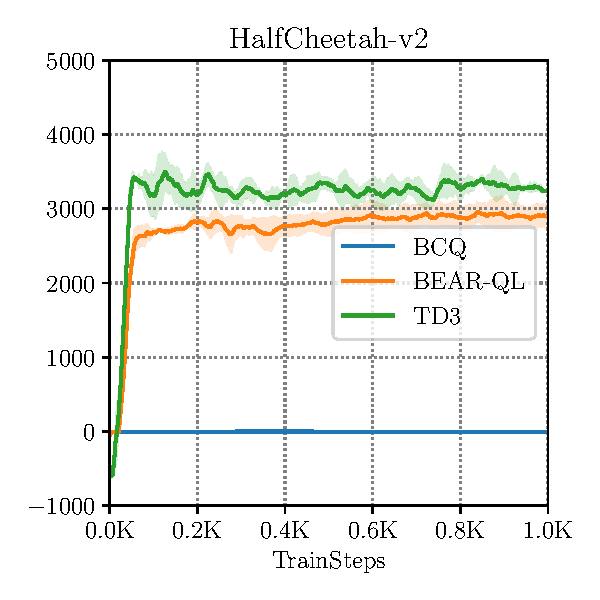
\includegraphics[width=0.99\linewidth]{chapters/bear/images/cheetah_random.pdf}
%         \caption{ }
%     \end{subfigure}%
%     ~ 
%     \begin{subfigure}[t]{0.23\textwidth}
%         \centering
%         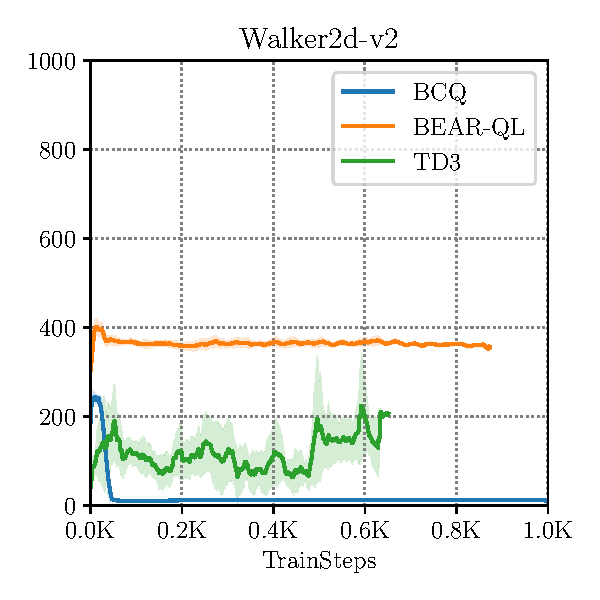
\includegraphics[width=0.99\linewidth]{chapters/bear/images/walker_random.pdf}
%         \caption{ }
%     \end{subfigure}
%     ~
%     \begin{subfigure}[t]{0.23\textwidth}
%         \centering
%         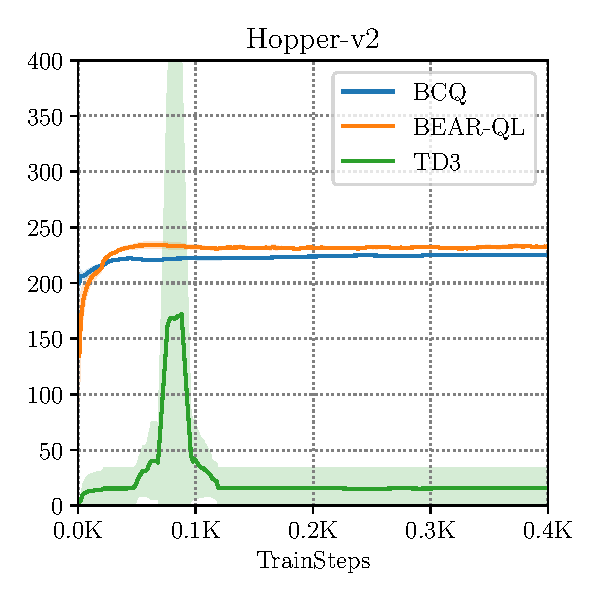
\includegraphics[width=0.99\linewidth]{chapters/bear/images/hopper_random.pdf}
%         \caption{ }
%     \end{subfigure}
%     ~
%     \begin{subfigure}[t]{0.23\textwidth}
%         \centering
%         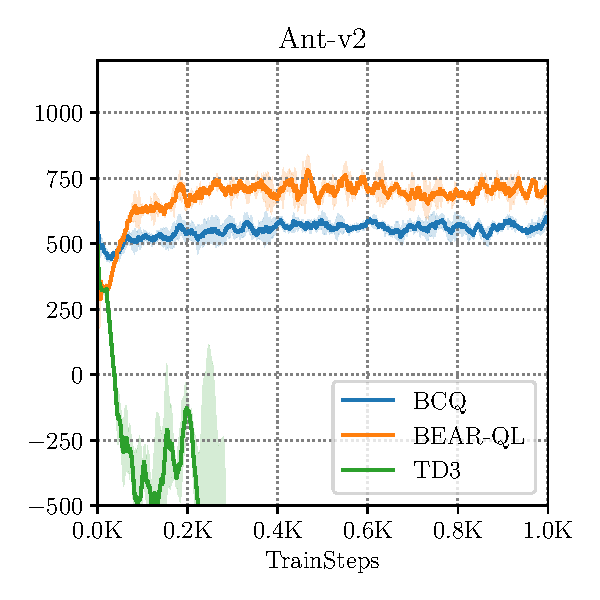
\includegraphics[width=0.99\linewidth]{chapters/bear/images/ant_mediocre.pdf}
%         \caption{ }
%     \end{subfigure}
%     \caption{Random Data}
% \end{figure*}

% \begin{figure*}[t!]
%     \centering
%     \begin{subfigure}[t]{0.23\textwidth}
%         \centering
%         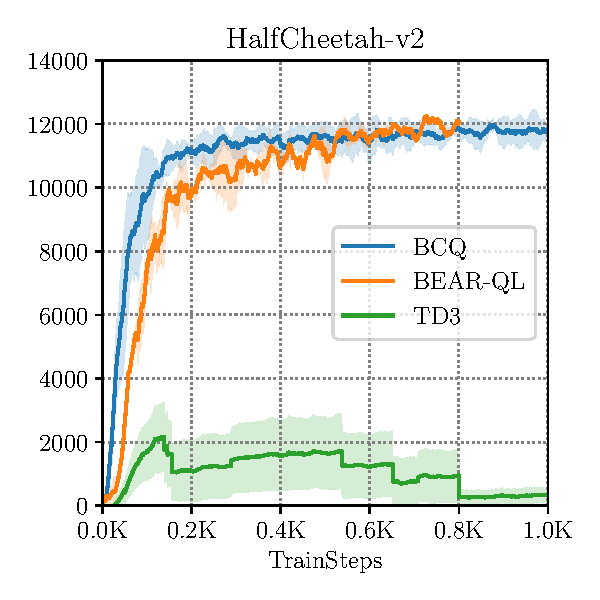
\includegraphics[width=0.99\linewidth]{chapters/bear/images/cheetah_optimal.pdf}
%         \caption{ }
%     \end{subfigure}%
%     ~ 
%     \begin{subfigure}[t]{0.23\textwidth}
%         \centering
%         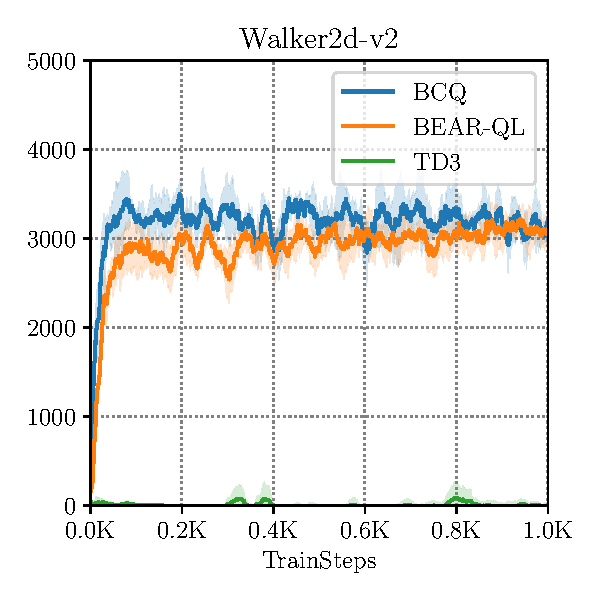
\includegraphics[width=0.99\linewidth]{chapters/bear/images/walker_optimal.pdf}
%         \caption{ }
%     \end{subfigure}
%     ~
%     \begin{subfigure}[t]{0.23\textwidth}
%         \centering
%         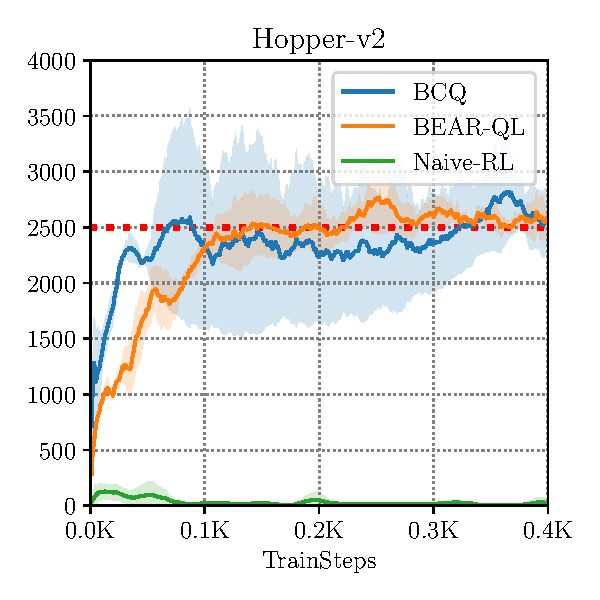
\includegraphics[width=0.99\linewidth]{chapters/bear/images/hopper_optimal.pdf}
%         \caption{ }
%     \end{subfigure}
%     ~
%     \begin{subfigure}[t]{0.23\textwidth}
%         \centering
%         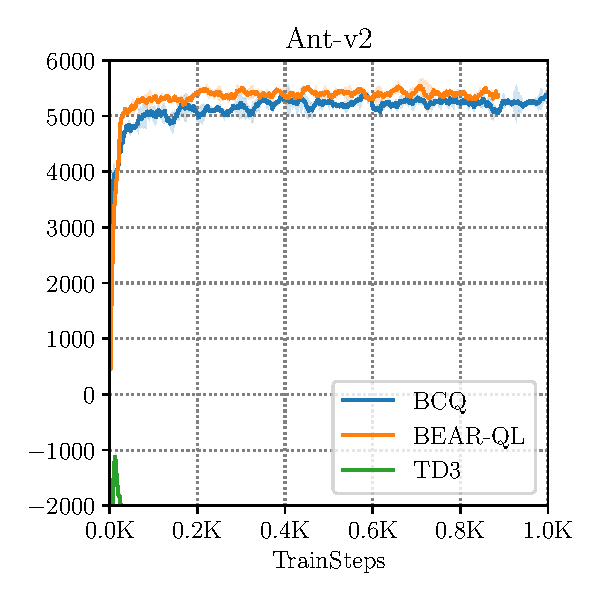
\includegraphics[width=0.99\linewidth]{chapters/bear/images/ant_optimal.pdf}
%         \caption{ }
%     \end{subfigure}
%     \caption{Optimal Data}
% \end{figure*}

\iffalse

\vspace{-5pt}
\subsection{Analysis of BEAR}
\label{subsec:ablations}
In this section, we aim to analyze different components of our method via an ablation study. Our first ablation studies the support constraint discussed in Section~\ref{sec:bear}, which uses MMD to measure support. We replace it with a more standard KL-divergence distribution constraint, which measures similarity in density. 
% \TODO{how is this done if we don't have the behavior policy? do you assume access for this study? -- we train a behavior policy on the data and then constrain to that with KL or MMD (so it should be a fair comparison)}
Our hypothesis is that this should provide a more conservative constraint, since matching distributions is not necessary for matching support. KL-divergence performs well in some cases, such as with optimal data, but as shown in Figure~\ref{fig:ablations}, it performs worse than MMD on medium-quality data. Even when KL-divergence is hand tuned fully, so as to prevent instability issues it still performs worse than a not-well tuned MMD constraint. We provide the results for this setting in the Appendix. We also vary the number of samples $n$ that are used to compute the MMD constraint. We find that smaller n ($\approx$ 4 or 5) gives better performance. Although the difference is not large, consistently better performance with 4 samples leans in favour of our hypothesis that an intermediate number of samples works well for support matching, and hence is less restrictive.

\fi
% Next, we study whether using a conservative Q-value estimate by subtracting the variance in the ensemble helps with learning. As shown in Figure~\ref{fig:ablations}, the conservative estimate 
%  makes a comparatively smaller difference than the use of MMD, providing some benefit on one task, while somewhat hurting performance on another.
% The ensemble produces more conservative estimates, which can result in underestimation in practice, and prevent overestimation divergence.

%The third factor in the ablation study is whether the usage of conservative estimates of Q-values subtracting the variance of the $Q$-ensemble helps. We find that on Hopper, usage of ensembles helps, whereas on Walker2d using ensembles hurts as the algorithm tends to underestimate Q-values. Figure~\ref{subfig:ensembles_ablation} demonstrates the average trend on 2 environments -- Hopper and Walker.




% \subsection{Generalization performance on datasets collected using a mixture of markovian policies.}
% We finally test our BEAR method in the case where the dataset $\dataset$ cannot be generated by a \TODO{Sergey and George: What's your opinion on having this section about non-markovian policies? This was one reason why Fujimoto got rejected. {https://openreview.net/forum?id=S1zlmnA5K7\&noteId=HJeQ-p0F2Q} }
% \TODO{Exp List: - Ant multiple + Point Mass multiple
%                 - with BCQ, BEAR, BEAR with n=1, BEAR without ensemble}

% \begin{figure}
%     \centering
%     \includegraphics{}
%     \caption{Caption}
%     \label{fig:my_label}
% \end{figure}
% \section{Discussion and Future Work}
\vspace{-5pt}
The goal in our work was to study off-policy reinforcement learning with static datasets. We theoretically and empirically analyze how error propagates in off-policy RL due to the use of out-of-distribution actions for computing the target values in the Bellman backup. Our experiments suggest that this source of error is one of the primary issues afflicting off-policy RL: increasing the number of samples does not appear to mitigate the degradation issue (Figure~\ref{fig:divergence}), and training with na\"{i}ve RL on data from a random policy, where there are no out-of-distribution actions, shows much less degradation than training on data from more focused policies (Figure~\ref{fig:optimal_random}). Armed with this insight, we develop a method for mitigating the effect of out-of-distribution actions, which we call BEAR-QL. BEAR-QL constrains the backup to use actions that have non-negligible support under the data distribution, but without being overly conservative in constraining the learned policy. We observe experimentally that BEAR-QL achieves good performance across a range of tasks, and across a range of dataset compositions, learning well on random, medium-quality, and expert data.

% \vspace{-0.15in}
\begin{wrapfigure}{r}{0.51\textwidth}
        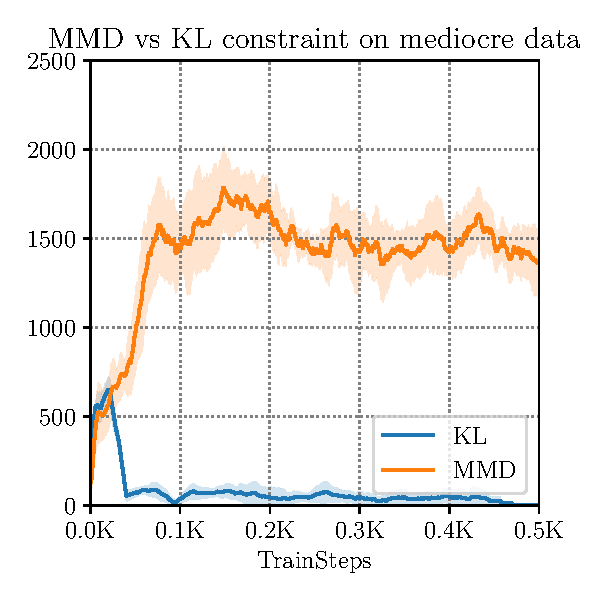
\includegraphics[width=0.48\linewidth]{chapters/bear/images/kl_vs_mmd_ablation_final.pdf}
       ~
        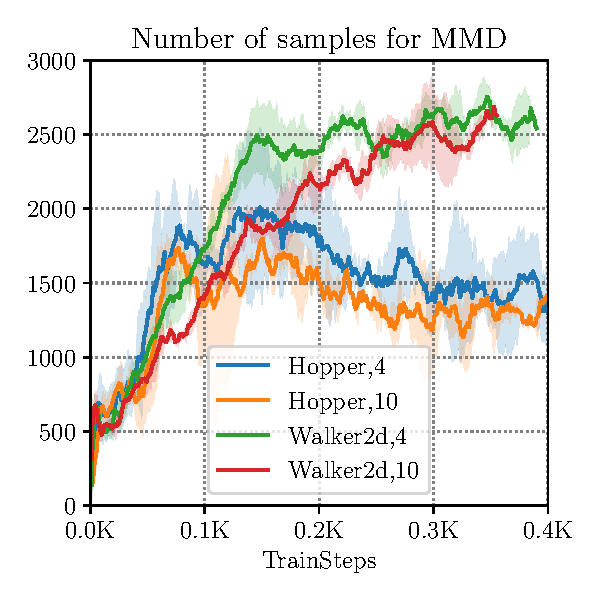
\includegraphics[width=0.48\linewidth]{chapters/bear/images/num_samples_ablation.pdf}
        % ~
        % \includegraphics[width=0.31\linewidth]{images/ensembles_ablation_final.pdf}
      \caption{\footnotesize Average return (averaged Hopper-v2 and Walker2d-v2) as a function of train steps for ablation studies from Section~\ref{subsec:ablations}. (a) MMD constrained optimization is more stable and leads to better returns, (b) 4 sample MMD is more performant than 10.}
    %   and (c) Ensemble variance has mixed benefit.}
      \label{fig:ablations}
\vspace{-10pt}
\end{wrapfigure}

While BEAR-QL substantially stabilizes off-policy RL, we believe that this problem merits further study. One limitation of our current method is that, although the learned policies are more performant than those acquired with na\"{i}ve RL, performance sometimes still tends to degrade for long learning runs. An exciting direction for future work would be to develop an early stopping condition for RL, perhaps by generalizing the notion of validation error to reinforcement learning. {A limitation of approaches that perform constrained-action selection is that they can be overly conservative when compared to methods that constrain state-distributions directly, especially with datasets collected from mixtures of policies. We leave it to future work to design algorithms that can directly constrain state distributions. A theoretically robust method for support matching efficiently in high-dimensional continuous action spaces is a question for future research. Perhaps methods from outside RL, predominantly used in domain adaptation, such as using asymmetric f-divergences~\citep{wu19domain} can be used for support restriction.} Another promising future direction is to examine how well BEAR-QL can work on large-scale off-policy learning problems, of the sort that are likely to arise in domains such as robotics, autonomous driving, operations research, and commerce. If RL algorithms can learn effectively from large-scale off-policy datasets, reinforcement learning can become a truly data-driven discipline, benefiting from the same advantage in generalization that has been seen in recent years in supervised learning fields, where large datasets have enabled rapid progress in terms of accuracy and generalization~\cite{imagenet_cvpr09}.

\section*{Acknowledgements}
We thank Kristian Hartikainen for sharing implementations of RL algorithms and for help in debugging certain issues. We thank Matthew Soh for help in setting up environments. We thank Aurick Zhou, Chelsea Finn, Abhishek Gupta, Kelvin Xu and Rishabh Agarwal for informative discussions. We thank Ofir Nachum for comments on an earlier draft of this paper. We thank Google, NVIDIA, and Amazon for providing computational resources. This research was supported by Berkeley DeepDrive, JPMorgan Chase \& Co., NSF IIS-1651843 and IIS-1614653, the DARPA Assured Autonomy program, and ARL DCIST CRA W911NF-17-2-0181.

% Q-learning methods are a common class of algorithms used in reinforcement learning (RL). However, their behavior with function approximation, especially with neural networks, is poorly understood theoretically and empirically. In this work, we aim to experimentally investigate potential issues in Q-learning, by means of a "unit testing" framework where we can utilize oracles to disentangle sources of error. 
% Specifically, we investigate questions related to function approximation, sampling error and nonstationarity, and where available, verify if trends found in oracle settings hold true with deep RL methods.
% We find that large neural network architectures have many benefits with regards to learning stability; offer several practical compensations for overfitting; and develop a novel sampling method based on explicitly compensating for function approximation error that yields fair improvement on high-dimensional continuous control domains. 

% \vspace{-0.4cm}
% \begin{AIbox}{\large{\textbf{Abstract}}}
% \vspace{4mm}
% In this chapter, we seek to understand challenges in the offline RL problem setting. To this end, we empirically study the behavior of off-policy RL methods when only training on a static, offline dataset. In principle, off-policy RL methods such as those based on approximate dynamic programming should succeed at leveraging experience collected from prior policies for sample-efficient learning. However, as we illustrate in this chapter, in practice, commonly used off-policy methods based on Q-learning and actor-critic are incredibly sensitive to \emph{both} the dataset distribution and quantity. Building on the insights from our empirical observations, we identify two main issues with learning value functions in the offline setting: \emph{distributional shift} and \emph{sampling error}. Later, we also demonstrate that these challenges also inhibit performance for other classes of off-policy RL methods such as model-based approaches. Finally, in subsequent chapters, we develop techniques to handle distributional shift, progressing towards reliable and easy-to-use offline RL algorithms.  
% \vspace{2mm}
% \end{AIbox}
    
% \vspace{-0.2cm}
\section{Introduction}
\vspace{-0.2cm}

In principle, off-policy reinforcement learning (RL) methods from Chapter~\ref{chapter:problem_statement} provide an effective way to learn optimal policies from static data: by learning value-functions, Q-learning and actor-critic algorithms, can learn optimal policies from even sub-optimal offline data. By attempting to isolate practical problems that hinder the usability of off-policy RL methods in learning from entirely static data, we wish to highlight challenges in offline RL. Specifically, we focus on answering the following questions: 

% Q-learning algorithms, which are based on approximating state-action value functions, are an efficient and commonly used class of RL methods. Q-learning methods have several very appealing properties: they are relatively sample-efficient when compared to policy gradient methods, and they allow for off-policy learning. This makes them an appealing choice for a wide range of tasks, from robotic control~\citep{kalashnikov18} and video game AI~\citep{Mnih2015} to off-policy learning from historical data for recommender systems~\citep{shani2005recommender}. However, although the basic tabular Q-learning algorithm is convergent and admits theoretical analysis~\cite{suttonrlbook}, its counterpart with function approximation is poorly understood. 
% In this paper, we aim to investigate the degree to which potential issues with Q-learning manifest in practice. 
% We empirically analyze aspects of the Q-learning method in a \emph{unit testing} framework, where we can employ oracle solvers to obtain ground truth Q-functions and distributions for exact analysis. We investigate the following questions:

% \textbf{1) What is the effect of function approximation on convergence?}
% Many practical RL problems require function approximation to handle large or continuous state spaces. However, the behavior of Q-learning methods under function approximation is not well understood -- there are simple counterexamples where the method diverges~\citep{Baird1995}. 
% To investigate these problems, we study the convergence behavior of Q-learning methods with function approximation by varying the function approximator power and analyzing the quality of the solution found. 
% We find, somewhat surprisingly, that divergence rarely occurs, and that function approximation error is not a major problem in Q-learning algorithms when the function approximator is powerful. This makes sense in light of the theory: a high-capacity approximator can perform an accurate projection of the bellman Backup, thus mitigating potential convergence issues due to function approximation. (Section~\ref{sec:function_approx})


\niparagraph{\large{(1) What is the effect of distributional shift?}}

% The standard formulation of off-policy Q-learning and actor-critic prescribes an update rule, with no corresponding objective function~\citep{Sutton09b}. This results in a learning process which optimizes an objective that suffers from distributional shift: the target values computed by the Bellman backup query actions from the learned policy, which is not necessarily identical to the data collection policy (and in general, we would expect that the learned policy would differ greatly from the data collection policy since it is supposed to improve over the behaviors in the offline dataset). We perform controlled experiments to investigate the amount of distributional shift and its impact on performance, observing that deviating away from the distributions of states and actions in the offline dataset can lead to significant instability over the course of learning.

The standard formulation of Q-learning and actor-critic prescribes a learning procedure that must make accurate counterfactul predictions about on states and actions visited by the learned policy. In general, the distribution of the learned policy will always be very different from that of the behavioral policy, and the difference will only be exacerbated for a correctly functioning algorithm that is able to find a policy close to the optimal policy for the problem. We perform controlled experiments to investigate the amount of distributional shift and its impact on performance, observing that deviating away from the distributions of states and actions in the offline dataset can lead to significant instability over the course of learning.



\niparagraph{\large{(2) What is the effect of sampling error?}}

In general, it is impossible to precisely infer the true underlying dynamical system using just a finite amount of offline data. This means that akin to standard supervised learning, off-policy RL algorithms that reuse a static dataset for learning would also overfit to the training data. To what extent, does this overfitting hurt performance? We experimentally show that overfitting exists in practice by performing ablation studies on the number of gradient steps utilized for learning, and by demonstrating that oracle based early stopping techniques can be used to improve performance of Q-learning algorithms.
%Thus, in our experiments we quantify the amount of overfitting which happens in practice, incorporating a variety of metrics, and performing a number of ablations and investigate methods to mitigate its effects.


% \textbf{4) What is the best sampling or weighting distribution?}
% Deeply tied to the distribution shift problem is the choice of which distribution to sample from. Do moving distributions cause instability, as Q-values trained on one distribution are evaluated under another in subsequent iterations?
% Researchers have often noted that on-policy samples are typically superior to off-policy samples~\citep{suttonrlbook}, and there are several theoretical results that highlight favorable convergence properties under on-policy samples. However, there is little theoretical guidance on how to pick distributions so as to maximize learning. To this end, we investigate several choices for the sampling distribution. {Surprisingly, we find that on-policy training distributions are not always preferable, and that broader, higher-entropy distributions often perform better, regardless of distributional shift. Motivated by our findings, we propose a novel weighting distribution, adversarial feature matching (AFM), which is explicitly compensates for function approximator error, while still producing high-entropy sampling distributions.}


%%AK: say this para in some different way
% In summary, we introduce a unit testing framework for Q-learning to disentangle potential bottlenecks where approximate components are replaced by oracles. This allows for controlled analysis of different sources of error. We study various sources of instability and error in Q-learning algorithms on tabular domains, and show that many of these trends hold true in high dimensional domains. We then propose a novel sampling distribution that improve performance even on high-dimensional tasks. %Our overall aim is to offer practical guidance for designing RL algorithms, as well as to identify important issues to solve in future research.

% % \section{Preliminaries}
\label{sec:backrgound}
Q-learning algorithms aim to solve a Markov decision process (MDP) by learning the optimal state-action value function, or Q-function. We define an MDP as a tuple $(\mathcal{S}, \mathcal{A}, \trans, R, \gamma)$. $\mathcal{S}, \mathcal{A}$ represent the state and action spaces, respectively. $\trans(s' | s, a)$ and $R(s,a)$ represent the dynamics (transition distribution) and reward function, respectively, and $\gamma \in (0,1)$ represents the discount factor. Letting $\rho_0(s)$ denote the initial state distribution, the goal in RL is to find a policy $\pi(a|s)$ that maximizes the expected cumulative discounted rewards, known as the \textit{returns}:
 $\pi^* = \argmax{\pi} E_{s_0 \sim \rho_0, s_{t+1} \sim \trans, a_t \sim \pi}\left[\sum_{t=0}^\infty \gamma^t R(s_t, a_t)\right] $
The quantity of interest in many Q-learning methods are the optimal state ($V^*(s)$) and state-action ($Q^*(s,a)$) value functions, which give the expected future return of the optimal policy starting from a particular state or state-action pair. Q-learning algorithms are based on iterating the Bellman backup operator $\backup$, defined as
\begin{align*}
(\backup Q)(s, a) &= R(s, a) + \gamma E_{s' \sim \trans}[V(s')]\\
V(s) &= \max_{a'} Q(s, a')
\end{align*}
Q-iteration is a dynamic programming algorithm that iterates the Bellman backup $Q^{t+1} \leftarrow \backup Q^t$. Because the Bellman backup is a $\gamma$-contraction in the $\linfnorm$ norm, and $Q^*$ is its fixed point, Q-iteration can be shown to converge to $Q^*$~\citep{suttonrlbook}. A deterministic optimal policy can then be obtained as $\pi^*(s) = \textrm{argmax}_{a} Q^*(s,a)$.

When state spaces are large, function approximation is needed to represent the Q-values. This corresponds to \textit{fitted Q-iteration} (FQI)~\citep{Ernst05}, a form of approximate dynamic programming (ADP), which forms the basis of modern deep RL methods such as DQN~\citep{Mnih2015}.
FQI projects the values of the Bellman backup onto a family of Q-function approximators $\Qclass$: $Q^{t+1} \leftarrow \Projmu(\backup Q^t)$.
$\Projmu$ denotes a $\mu$-weighted $\ltwonorm$ projection, which minimizes the \textit{Bellman error} via supervised learning:
\begin{equation}
\label{eqn:bellman_projection} 
\Projmu(Q) \defeq 
\argmin{Q' \in \Qclass} E_{s,a \sim \mu}[(Q'(s,a) - Q(s,a))^2]
 .\end{equation}
The values produced by the Bellman backup, $(\backup Q^t)(s,a)$ are commonly referred to as \textit{target values}, and when neural networks are used for function approximation, the previous Q-function $Q^t(s,a)$ is referred to as the \textit{target network}. In this work, we distinguish between the cases when the Bellman error is estimated with Monte-Carlo sampling or computed exactly (see Section~\ref{sec:setup_algos}). The sampled variant corresponds to FQI as described in the literature~\citep{Ernst05,Riedmiller2005}, while the exact variant is an example of conventional ADP methods~\citep{Bertsekas96}. 
Convergence guarantees for Q-iteration do not cleanly translate to FQI. $\Projmu$ is an $\ltwonorm$ projection, but $\backup$ is a contraction in the $\linfnorm$ norm -- this norm mismatch means the composition of the backup and projection is no longer guaranteed to be a contraction under any norm~\citep{Bertsekas96}, and hence convergence is not guaranteed.

A related branch of Q-learning methods are \textit{online Q-learning} methods,
in which Q-values are updated while samples are being collected in the MDP. This includes classic algorithms such as Watkin's Q-learning~\citep{Watkins1992}. Online Q-learning methods can be viewed as a form of stochastic approximation applied to Q-iteration and FQI~\citep{Bertsekas96}, and share many of its theoretical properties~\citep{tsitsiklis1994asynchronous,szepesvari1998asymptotic}.
Modern deep RL algorithms such as DQN~\citep{Mnih2015} have characteristics of both online Q-learning and FQI -- using replay buffers means the sampling distribution $\mu$ changes very little between target updates (see Section~\ref{sec:distr_shift}), and target networks are justified from the viewpoint of FQI. Because FQI corresponds to the case when the sampling distribution is static between target updates, the behavior of modern deep RL methods more closely resembles FQI than a true online method without target networks.


% \vspace{-0.2cm}
\section{Experimental Setup}
\label{sec:diagnosing_setup}
\vspace{-0.2cm}
% Our experimental setup is centered around \emph{unit-testing}. We evaluate a spectrum of Q-learning algorithms, starting with exact dynamic programming and replacing exact components with practical approximations, until the algorithm resembles modern deep Q-learning methods. 
% %We then introduce a suite of tabular environments where oracle solutions can be computed, to aid in diagnosis, as well as testing in high-dimensional environments to verify our hypotheses.

While it is definitely possible to study challenges with off-policy RL methods in offline RL on common deep RL benchmark tasks (e.g., OpenAI Gym~\citep{gym} environments), these tasks do not necessarily provide us with the ability to compute oracle solutions and isolate challenges individually. Therefore, we perform our study in a ``unit-testing'' setup, consisting of gridworld and other tabular environments with varying difficulty levels, where it is possible to compute oracle solutions and control for different factors independently.
% We release this suite of tasks at: \url{https://github.com/justinjfu/diagnosing_qlearning}.    


% \iffalse

% \subsection{Algorithms}
% \label{sec:setup_algos}
% We use three different Q-learning variants, each of which controls for a specific source of approximation error -- 
% Exact-FQI, Sampling-FQI, and Replay-FQI. 
% We use FQI as a basis for our controlled analysis, as it strongly resembles modern deep RL algorithms while allowing us to separately isolate target values, update rates, and the number of samples used for each iteration. We then confirm that the observed trends hold with several state-of-the-art deep RL methods (SAC~\citep{Haarnoja2017}, TD3~\citep{pmlr-v80-fujimoto18a}) on standard benchmark problems.
% %Although FQI is not exactly identical to commonly used deep RL methods, such as DQN~\citep{Mnih2015}, DDPG~\citep{Lillicrap2015},TD3~\citep{pmlr-v80-fujimoto18a}, and SAC~\citep{Haarnoja2017}, it is structurally similar and, when the replay buffer for the commonly used methods becomes large, the difference becomes negligible, since the sampling distribution changes very little between target network updates. 
% %However, FQI methods are much more amenable for controlled analysis, since we can separately isolate target values, update rates, and the number of samples used for each iteration. We therefore use variants of FQI as the basis for our analysis, but we also confirm that similar trends hold with more commonly used algorithms on standard benchmark problems.

% \begin{figure*}[ttt!]
% \begin{small}
% \begin{minipage}[t]{0.33\linewidth}
% \begin{algorithm}[H]
% \small
% \caption{Exact-FQI}
% \label{alg:fqiexact}
% \begin{algorithmic}[1]
%     \STATE Initialize Q-value approximator $Q_\theta(s,a)$.
%     \FOR{step $t$ in \{1, \dots, N\}}
%         \item[]
%         \item[]
%         \item[]
%         \STATE Evaluate $Q_{\theta^t}(s,a)$ at all states.
%         \STATE Compute exact target values at all states. \\
%         $y(s,a) = r(s,a) + \gamma E_{s'}[ V_{\theta^t}(s')]$ 
%         \STATE Minimize projection loss with respect to $\mu$: \\
%         $\argmin{\theta} E_\mu[(Q_\theta(s,a) - y(s,a))^2]$
%     \ENDFOR
% \end{algorithmic}
% \end{algorithm}
% \end{minipage}
% \begin{minipage}[t]{0.33\linewidth}
% \begin{algorithm}[H]
% \small
% \caption{Sampled-FQI}
% \label{alg:fqisampled}
% \begin{algorithmic}[1]
%     \STATE Initialize Q-value approximator $Q_\theta(s,a)$.
%     \FOR{step $t$ in \{1, \dots, N\}}
%         \item[]
%         \item[]
%         \STATE \textdiff{Collect $M$ samples from $\mu$.}
%         \STATE Evaluate $Q_{\theta^t}(s,a)$ \textdiff{on samples.}
%         \STATE Compute sampled target values \textdiff{on samples.}\\
%         $\hat{y}_i = r_i + \gamma V_{\theta^t}(s'_i)$ 
%         \STATE Minimize projection loss with respect to \textdiff{samples}: \\
%         $ \argmin{\theta} \frac{1}{M}\sum_{i=1}^M (Q_\theta(s_i,a_i) - y_i)^2$
%     \ENDFOR
% \end{algorithmic}
% \end{algorithm}
% \end{minipage}
% \begin{minipage}[t]{0.33\linewidth}
% \begin{algorithm}[H]
% \small
% \caption{Replay-FQI}
% \label{alg:fqireplay}
% \begin{algorithmic}[1]
%     \STATE Initialize Q-value approximator $Q_\theta(s,a)$, \textdiff{replay buffer $\ReplayBuffer$}.
%     \FOR{step $t$ in \{1, \dots, N\}}
%         \STATE \textdiff{Collect $K$ online samples from $\mu$.}
%         \STATE \textdiff{Append online samples to buffer $\ReplayBuffer$.}
%         \STATE Collect $M$ samples from $\ReplayBuffer$.
%         %\STATE \textbf{Collect $K$ replay samples $(s_k, a_k, s'_k, r_k)$ from $\ReplayBuffer$}.
%         \STATE Evaluate $Q_{\theta^t}(s,a)$ on samples.
%         \STATE Compute sampled target values on samples\\
%         $\hat{y}_i = r_i + \gamma V_{\theta^t}(s'_i)$ 
%         \STATE Minimize projection loss with respect to samples: \\
%         $ \argmin{\theta} \frac{1}{M}\sum_{i=1}^M (Q_\theta(s_i,a_i) - y_i)^2$
%     \ENDFOR
% \end{algorithmic}
% \end{algorithm}
% \end{minipage}
% \end{small}
% \end{figure*}


% \textbf{Exact-FQI} (Algorithm~\ref{alg:fqiexact}): Exact-FQI uses known dynamics and reward functions and computes the backup and projection on all state-action tuples, without sampling error. We use Exact-FQI to study convergence, distribution shift (by varying weighting distributions on transitions), and function approximation in the absence of sampling error. 
% %Exact-FQI eliminates errors due to sampling states, and computing inexact, sampled backups.

% \textbf{Sampled-FQI} (Algorithm~\ref{alg:fqisampled}): Sampled-FQI is a special case of Exact-FQI,
% where the Bellman error is approximated with Monte-Carlo estimates from a sampling distribution $\mu$, and the Bellman backup is approximated with samples from the dynamics as $r(s,a) + \gamma \max_{a'}Q(s', a')$. We use Sampled-FQI to study effects of overfitting. Sampled-FQI incorporates errors arising from function approximation, sampling, and distribution shift.

% \textbf{Replay-FQI} (Algorithm~\ref{alg:fqireplay}): Replay-FQI is a special case of Sampled-FQI that uses a \textit{replay buffer}~\citep{lin1992replay},
% that saves past transition samples $(s, a, s', r)$, which are used for computing Bellman error. Replay-FQI strongle resembles DQN~\cite{Mnih2015}, but lacking the online updates that allow $\mu$ to change within an FQI iteration. 
% With large replay buffers, we expect the difference between Replay-FQI and DQN to be minimal as $\mu$ changes slowly.

% We additionally investigate the following choices of weighting distributions ($\mu$) for the Bellman error:
% %When sampling the Bellman error, these can be implemented by sampling directly from the distribution, or via importance sampling.

% \textbf{Unif$(s,a)$}: Uniform weights over state-action space. 
% %This is the weighting distribution typically used by dynamic programming algorithms, such as FQI.

% \textbf{$\pi(s,a)$}: The on-policy state-action marginal induced by $\pi$.

% \textbf{$\pi^*(s,a)$}: The state-action marginal induced by $\pi^*$.

% \textbf{Random$(s,a)$}: State-action marginal induced by executing uniformly random actions.

% \textbf{Prioritized$(s,a)$}: Weights Bellman errors proportional to $|Q(s,a)-\backup Q(s,a)|$. This is similar to prioritized replay~\citep{Schaul2015} with $\beta=0$.

% \textbf{Replay$(s,a)$} and \textbf{Replay10$(s,a)$}: Averaged state-action marginal of all policies (or the last 10) produced during training. This simulates sampling from a replay buffer. 

% \fi


For our study, we selected eight tabular domains, each with different qualitative attributes, including: gridworlds of varying sizes and observations, blind Cliffwalk~\citep{Schaul2015}, discretized Pendulum and Mountain Car based on OpenAI Gym~\citep{gym},
and a sparsely connected graph. We discuss each domain in detail below:

\begin{itemize}

\item \textbf{Gridworlds}. The Gridworld environment is an NxN grid with randomly placed walls. The reward is proportional to Manhattan distance to a goal state (1 at the goal, 0 at the initial position), and there is a 5\% chance the agent travels in a different direction than commanded. We vary two parameters: the size ($16 \times 16$ and $64 \times 64$), and the state representations. We use a one-hot representation, an (X, Y) coordinate tuple (represented as two one-hot vectors), and a random representation, a vector drawn from $\mathcal{N}(0, 1)^N$, where N is the width or height of the Gridworld. The random observation significantly increases the challenge of function approximation, as significant state aliasing occurs.

\item \textbf{Cliffwalk}: Cliffwalk is a toy example from \citet{Schaul2015}. It consists of a sequence of states, where each state has two allowed actions: advance to the next state or return to the initial state. A reward of 1.0 is obtained when the agent reaches the final state. Observations consist of vectors drawn from $\mathcal{N}(0, 1)^{16}$.

\item \textbf{InvertedPendulum and MountainCar}: InvertedPendulum and MountainCar are discretized versions of continuous control tasks found in OpenAI gym~\citep{gym}, and are based on problems from classical RL literature. In the InvertedPendulum task, an agent must swing up an pendulum and hold it in its upright position. The state consists of the angle and angular velocity of the pendulum. Maximum reward is given when the pendulum is upright. The observation consists of the $\sin$ and $\cos$ of the pendulum angle, and the angular velocity. In the MountainCar task, the agent must push a vehicle up a hill, but the hill is steep enough that the agent must gather momentum by swinging back and forth within a valley in order to reach the top. The state consists of the position and velocity of the vehicle.

\item \textbf{SparseGraph}: The SparseGraph environment is a 256-state graph with randomly drawn edges. Each state has two edges, each corresponding to an action. One state is chosen as the goal state, where the agent receives a reward of one.

\end{itemize}

\noindent In order to provide consistent metrics across domains, we normalize returns and errors involving Q-functions by the returns of the expert policy $\pi^*$ on each environment. 

% \subsection{Function Approximators}
% Throughout our experiments, we use 2-layer ReLU networks, denoted by a tuple $(N, N)$ where N represents the number of units in a layer. The ``Tabular'' architecture refers to the case when no function approximation is used. 

% \subsection{High-Dimensional Testing}

% In addition to diagnostic experiments on tabular domains, we also wish to see if the observed trends hold true on high-dimensional environments. Thus, we include experiments on continuous control tasks in the OpenAI Gym benchmark~\citep{gym} (HalfCheetah-v2, Hopper-v2, Ant-v2, Walker2d-v2). In continuous domains, computing the maximum over actions of the Q-value is difficult ($\max_a Q(s,a)$). A common choice in this case is to use an ``actor'' function to approximate $\arg\max_a Q(s,a)$~\cite{Lillicrap2015,pmlr-v80-fujimoto18a,Haarnoja18}. This approach resembles Replay-FQI, but using the actor network in place of the max.
%\vspace{-20pt}
% % \section{Function Approximation and Convergence}
\label{sec:function_approx}

%The first issue we investigate is the connection between function approximation and convergence properties.

%\subsection{Technical Background}
This interaction between approximation and convergence has been a long-studied topic in RL and ADP. In control theory, it is closely related to the problems of state-aliasing or interference~\citep{Farrell95}. \citet{Baird1995} introduces a counterexample in which Watkin's Q-learning with linear approximators causes unbounded divergence. However, several works have noted that divergence need not occur. \citet{munos2005erroravi,antos2008concentrability,farahmand2010error} address the norm-mismatch problem by showing convergence guarantees in $\lpnorm$-norms, at the price of introducing a \textit{concentrability coefficient} that worsens the error bound (and is potentially infinite for deterministic MDPs). In policy evaluation, \citet{Tsitsiklis1997} prove that on-policy TD-learning with linear approximators converges, and methods such as GTD~\citep{Sutton09b} and ETD~\citep{Sutton2016} have extended results to off-policy cases.
In the control scenario, convergent algorithms such as SBEED~\citep{Dai2018} and Greedy-GQ~\citep{Maei2010} have been developed. Concurrently to us,\citet{VanHesselt2018} experimentally find that unbounded divergence rarely occurs with DQN variants on Atari games. 

\subsection{How does function approximation affect convergence and solution suboptimality?}
The crucial quantities we wish to measure are a trend between function approximation and performance, and a measure for the bias in the learning procedure introduced by function approximation.
Using Exact-FQI with uniform weighting (to remove sampling error), we plot the returns of the learned policy, and the $\linfnorm$ error between $Q^*$ and the solution found by Exact-FQI ($\lim_{t \to \infty} (\Projmu \backup)^t Q^0$) and the projection of the optimal solution  ($\Projmu Q^*$) in Fig.~\ref{fig:function_approx}. $\Projmu Q^*$ represents the best solution within model class, in absence of bootstrapping error. Thus, the difference between FQI error and projection error represents the additional bias introduced by FQI (the \textit{inherent Bellman error} of the function class~\citep{munos2008finite}). This is the potential gap that can be improved via better algorithm design.

\begin{figure}
\vspace{-0.5cm}
\caption{\label{fig:function_approx} Normalized returns and Q-function error with function approximation, averaged across domains and seeds. Small architectures show a large gap between the solution found by FQI (FQI Error) and the best solution within model class (Project Error).}
\centering
\includegraphics[width=0.7\linewidth]{chapters/diagnosing_q/images/fig_1.pdf}
% generated by plot_doodad_exact_fqi.py:returns_qstar_vs_arch
% data_dir = east1//2019-01-18-newenv-exact-weighting
\vspace{-0.8cm}
\end{figure}

We first note the obvious trend that smaller architectures produce lower returns and converge to worse solutions. 
However, we also find that smaller architectures introduce significant bias in the \textit{learning process}, and there is a significant gap between the solution found by Exact-FQI and the best solution within the model class. 
One explanation is that when the target is bootstrapped, we must represent all Q-functions along the path to the solution, and not only the final result~\citep{Bertsekas96}.
This observation implies that using large architectures is crucial not only because they have capacity to represent a better solution, but also because they are easier to train using bootstrapping. 
We also note that divergence rarely occurs in practice, occuring in only 0.9\% of our experiments (measured as the Q-values growing larger than 10 times $Q^*(s,a)$). 

For high-dimensional problems, we present experiments on varying the architecture of the Q-network in SAC~\cite{Haarnoja18} in Appendix Fig.~\ref{fig:size_sac}. We still observe that large networks have the best performance, and that divergence rarely happens even in high-dimensional continuous spaces. We briefly discuss theoretical intuitions on apparent discrepancy between the lack of unbounded divergence in relation known counterexamples in Appendix~\ref{app:bounded_error}.

% \vspace{-0.2cm}
\section{Impact of Distributional Shift}
\label{sec:sampling_distributions}
\vspace{-0.2cm}

%As alluded to in Section~\ref{sec:analysis_nonstationarity}, the choice of sampling distribution $\mu$ is an important design decision can have a large impact on performance. Indeed, it is not immediately clear which distribution is ideal for Q-learning. In this section, we hope to shed some light on this issue.

%\subsection{Technical Background}
% Off-policy data has been cited as one of the ``deadly triads'' for Q-learning~\citep{suttonrlbook}, which has potential to cause instabilities in learning. On-policy distributions~\citep{Tsitsiklis1997} and fixed behavior distributions~\citep{Sutton09a,Maei2010} have often been targeted for theoretical convergence analysis, and many works use importance sampling to correct for off-policyness~\citep{precup2001offpol, munos2016safe}
% However, to our knowledge, there is relatively little guidance which compares how different weighting distributions compare in terms of convergence rate and final solutions.

% Off-policy RL methods applied to the offline RL problem would typically attempt to learn an optimal policy, even though the static dataset may not be generated from an optimal policy. As a result, one issue to emerge is that of \emph{distributional shift}: while these methods can only train a model of the value-function and the policy using state-action tuples from the data, these models  will need to make correct predictions on states and actions sampled from a different distribution encountered upon deployment. In general, models trained via machine learning are not robust when the distribution of inputs changes, indicating that distributional shift can be challenge for off-policy RL methods. Is distributional shift a challenge in offline RL?   

Off-policy RL methods applied to the offline RL problem would typically attempt to learn an optimal policy, even though the static dataset may not be generated from an optimal policy. As a result, one issue that emerges is that of \emph{distributional shift}: while these methods train a model of the value-function and the policy only using state-action tuples from the data, upon deployment, these models will need to make correct predictions on states and actions sampled from a different distribution of the learned policy. In general, models trained via machine learning are not robust when the distribution of inputs changes, indicating that distributional shift can be a challenge for off-policy RL methods. Is distributional shift a challenge in offline RL?

Indeed, theoretically, the effects of distributional shift have been quantified using the notion of a concentrability coefficient~\citep{munos2005erroravi}, a constant typically $\gg 1$, which provides a worst-case error bound on the performance of an off-policy RL method due to distributional shift. To evaluate if this challenge persists empirically as well, we will analyze Q-learning methods for various choices of data distributions in this section.

A crucial design decision we must make is to consider setups that do not confound distributional shift with access to limited data. Therefore, for our study, we provide the underlying algorithm oracle access to all state-action transitions in the MDP, but vary the \emph{distribution} over state-action pairs from which these transitions are sampled.

% Indeed, theoretically, the effects of distributional shift have been quantified using the notion of a concentrability coefficient~\citep{munos2005erroravi}, a constant typically $\ggt 1$, which provides a worst-case error bound on the performance of an off-policy RL method due to distributional shift. To evaluate if this challenge persists empirically as well, we will analyze Q-learning methods for various choices of data distributions in this section. 

% A crucial design decision we must make is to consider setups that do not confound distributional shift with access to limited data. Therefore, for our study, we provide the underlying algorithm oracle access to all state-action transitions in the MDP, but vary the \emph{distribution} over state-action pairs that these transitions are sampled according to.   
% ~\citep{NIPS2017_6913} suggests that when the state-distribution is fixed, the action distribution should be weighted by the optimal policy for residual Bellman errors. In deep RL, prioritized replay~\citep{Schaul2015}, and mixing replay buffer with on-policy data~\citep{hausknecht2016policy,zhang2018deeper} have been found to be effective. %We aim to empirically analyze multiple choices for weighting distributions to determine which are the most effective.

%\vspace{-10pt}
\vspace{-0.2cm}
\subsection{What Are the Best Data Distributions Without Sampling Error?}
\label{subsec:dist_shift_exact}
\vspace{-0.2cm}

% \begin{figure*}[ttt!]
% \begin{subfigure}{0.3\linewidth}
% \caption{\footnotesize \label{fig:distribution_shift_vs_returns} Average distribution shift across time for different data distributions, plotted against returns for a 256x256 model. We find that distribution shift does not have strong correlation with returns.}
% \includegraphics[width=0.99\columnwidth]{chapters/diagnosing_q/images/returns_vs_shift}
% % generated by plot_distribution_shift.py
% % data_dir = east1//2019-02-12-exact-weighting-distr-shift
% \vspace{-0.2in}
% \end{subfigure}
% ~\vline~
% \begin{subfigure}{0.3\linewidth}
% \caption{\footnotesize \label{fig:weighting_schemes} Weighting distribution versus architecture in Exact-FQI. Replay(s, a) consistently provides the highest performance. Note that Adversarial Feature Matching is comparable to Replay(s, a), but surprisingly better for small networks. }
% \includegraphics[width=0.99\columnwidth]{chapters/diagnosing_q/images/exact_fqi_schemes.pdf}
% % generated by plot_exact_weighting.py
% % data_dir = east1//2019-01-18-newenv-exact-weighting
% \vspace{-0.3in}
% \end{subfigure}
% ~\vline~
% \begin{subfigure}{0.3\linewidth}
% \caption{\footnotesize \label{fig:weighting_entropy_vs_returns} Normalized returns plotted against normalized entropy for different weighting distributions. All experiments use Exact-FQI with a 256x256 network. We see a general trend that high-entropy distributions lead to greater performance.}
% \includegraphics[width=0.99\columnwidth]{chapters/diagnosing_q/images/returns_vs_entropy}
% % generated by plot_distribution_shift.py
% % data_dir = east1//2019-02-12-exact-weighting-distr-shift
% \end{subfigure}
% \end{figure*}

\begin{wrapfigure}{r}{0.45\linewidth}
    \vspace{-0.2cm}
    \includegraphics[width=0.99\linewidth]{chapters/diagnosing_q/images/returns_vs_entropy}
    \caption{\footnotesize \label{fig:weighting_entropy_vs_returns} Normalized returns plotted against normalized entropy for different weighting distributions. All experiments assume access to all state-action pairs with a 256x256 Q-network. We see a general trend that high-entropy distributions lead to greater performance, corroborating the uniformity hypothesis.}
    \vspace{-0.2cm}
    % generated by plot_distribution_shift.py
    % data_dir = east1//2019-02-12-exact-weighting-distr-shift
\end{wrapfigure}
We begin by studying the effect of data distributions when disentangled from sampling error. We run Q-learning with an ablation over various Q-function network architectures and data distributions and report our aggregate results in Fig.~\ref{fig:weighting_entropy_vs_returns}. $\text{Unif}(\bs, \mathbf{a})$, $\text{Replay}(\bs, \mathbf{a})$ (using a replay buffer consisting of data from a mixture of policies with different degrees of optimality), and $\text{Prioritized}(\bs, \mathbf{a})$ (weighting induced by prioritized experience replay~\citep{Schaul2015}) consistently result in the highest returns across all architectures. On the other hand, relatively ``narrow'' data distributions, such as those induced the optimal policy ($\pi^*$) or only using a mixture of a few policies ($\text{Replay}(10)$) results in poor performance.
% We believe that these results are in favor of the \textit{uniformity} hypothesis: intuitively, the best distributions spread weight across larger support of the state-action space, reducing the amount of possible distributional shift. On the other hand, less-uniform distributions such as the state-action distirbution induced by the optimal policy, present multiple avenues to deviate away from the offline data distribution, resulting in larger distributional shift.
We believe that these results favor the \textit{uniformity} hypothesis: intuitively, the best distributions spread weight across a larger support of the state-action space, reducing the amount of possible distributional shift. On the other hand, less-uniform distributions, such as the state-action distribution induced by the optimal policy, present multiple avenues to deviate away from the offline data distribution, resulting in larger distributional shift.

\textbf{To summarize}, this indicates that narrow data distributions lead to worse performance compared to higher-entropy data distributions, indicating that distributional shift can have a significant impact on the performance of off-policy RL in the offline setting.
%These distributions generally result in the tightest contraction rates, and allow the Q-function to focus on high-error regions. 
%In the sampled setting, this observation motivates exploration algorithms that maximize state coverage (for example, ~\citet{hazan2018} solve an exploration objective which maximizes state-space entropy).
%However, note that in this particular experiment is distinct from exploration, as there is no sampling involved. 
%All states are observed, just with different weights, thus isolating the issue of distributions from the issue of sampling.
% \section{Question 2: What is the Impact of Sampling Error and Overfitting?}
\label{sec:overfitting}

%A second source of error in minimizing the Bellman error, orthogonal to function approximation, is that of sampling or generalization error. The next issue we investigate is the effect of sampling error on Q-learning methods.

%\subsection{Technical Background}

Thus far, we have observed that the performance of off-policy RL algorithms based on Q-learning can be quite sensitive to the distribution of the offline dataset, even when all the transition tuples in the MDP are provided to the algorithm and only the weighting over these samples is varied. In this section, we aim to study a distinct question: we study
\begin{wrapfigure}{r}{0.5\linewidth}
    \centering
    \vspace{-10pt}
    \includegraphics[scale=0.4]{chapters/diagnosing_q/images/samples_arch.pdf}
    \vspace{-0.2cm}
    \caption{\label{fig:sampling_256} Samples plotted with returns for a 256x256 network. More samples yields better performance.}
    \vspace{-0.5cm}
    %plot_sampling
    %east1//2019-01-20-newenv-sample-weighting
\end{wrapfigure}
\!\!the performance of off-policy Q-learning when the offline dataset is of a finite size, and may not contain all transitions in the MDP. To address any confounders from distributional shift, we provide the underlying Q-learning algorithm oracle access to collecting a limited amount of data from the current snapshot of the learned policy. While this sort of active data collection is not possible in the offline RL problem setting, we find that it allows us to more carefully localize the challenges of overfitting and sampling error.

% Approximate dynamic programming assumes that the projection of the Bellman backup (Eqn.~\ref{eqn:bellman_projection}) is computed exactly, but in reinforcement learning we can normally only compute the \textit{empirical Bellman error} over a finite set of samples. In the PAC framework, overfitting can be quantified by a bounded error in between the empirical and expected loss with high probability, which decays with sample size~\citep{Shalev2014}. \citet{munos2008finite, maillard2010finite, tosatto2017boosted} provide such PAC-bounds which account for sampling error in the context of Q-learning and value-based methods, and quantify the quality of the final solution in terms of sample complexity.

We analyze several key points that relate to sampling error. First, we show that Q-learning is prone to overfitting, and that this overfitting has a real impact on performance. 

\subsection{Quantifying Overfitting}
We first quantify the amount of overfitting that happens during training, by varying the number of samples. In order provide comparable validation errors across different experiments, we fix a reference sequence of Q-functions, $Q^1, ... , Q^N$, obtained during an arbitrary run of Q-learning. We then retrace the training sequence, and minimize the projection error $\Projmu(Q^t)$ at each training iteration, using varying amounts of on-policy data or sampling from a replay buffer. We measure the validation error (the expected Bellman error) at each iteration under the on-policy distribution, plotted in Figure~\ref{fig:sampling_validation_loss}. We note the obvious trend that more samples leads to significantly lower validation loss. 
% A more interesting observation is that sampling from the replay buffer results in the lowest on-policy validation loss, despite bias due to distribution mismatch from sampling off-policy data. As we elaborate in Section~\ref{sec:analysis_nonstationarity}, we believe that replay buffers are effective because they reduce overfitting and have good sample coverage over the state space, not necessarily due to reducing the effects of nonstationarity.

Next, Figure~\ref{fig:sampling_256} shows the relationship between number of samples and returns. We see that more samples leads to improved learning speed and a better final solution. A full sweep including architectures is presented in the Appendix (Figure~\ref{fig:sampling_arch_sweep}). Despite overfitting being an issue, larger architectures still perform better because the bias introduced by smaller architectures dominates. This observation indicate that the nature of overfitting in RL is likely significantly different from that of supervised learning: while overfitting in supervised learning can bne controlled by regulating model capacity, off-policy RL methods likely need to rely on alternative techniques to control overfitting. We have made some progress towards understanding this questions in \citet{li2022effective}.   

\begin{figure*}[ttt!]
\begin{subfigure}{0.31\linewidth}
\includegraphics[width=0.97\linewidth]{chapters/diagnosing_q/images/overfitting.pdf}
%plot_overfitting
%central1//2019-01-21-overfitting-coupled
\caption{\label{fig:sampling_validation_loss} On-policy validation losses for varying amounts of on-policy data (or replay buffer), averaged across environments and seeds. Note that sampling from the replay buffer has lower on-policy validation loss, despite bias from distribution shift.}
\end{subfigure}
~\vline~
\begin{subfigure}{0.31\linewidth}
\includegraphics[trim={0 0 7.0cm 0},clip,width=0.97\linewidth]{chapters/diagnosing_q/images/grad_steps_fqi}
%plot_overfitting
%central1//2019-01-21-overfitting-coupled
\caption{\label{fig:fqi_grad_sweep}Normalized returns plotted over training iterations (32 samples per iteration), for different ratios of gradient steps per sample. We observe that intermediate values of gradient steps work best, and too many gradient steps hurt performance.}
\end{subfigure}
~\vline~
\begin{subfigure}{0.31\linewidth}
\includegraphics[trim={0 0 4.4cm 0},clip,width=0.97\linewidth]{chapters/diagnosing_q/images/validation_stop}
%plot_validation_stop
%west1//2019-02-20-replay-validation-stop
\caption{\label{fig:validation_stop}Normalized returns plotted over training iterations (32 samples are taken per iteration), for different early stopping methods. We observe that using proper early stopping can result in a modest performance increase.}
\end{subfigure}
\end{figure*}

\subsection{Does Compensating for Overfitting Improve Performance?}

Finally, to confirm our hypotheses regarding overfitting, we now wish to understand if compensating for overfitting does lead to improved performance. One common technique for reducing overfitting is to utilize \textit{early stopping} methods to mitigate overfitting without reducing model size.
% We first note that the number of gradient steps taken per sample in the projection step has an important effect on performance -- too few steps and the algorithm learns slowly, but too many steps and the algorithm may initially learn quickly but overfit. To show this, we run an ablation over the number of gradient steps taken per sample in Replay-FQI and TD3 (TD3 uses 1 by default). Results for FQI are shown in Fig.~\ref{fig:fqi_grad_sweep}, and for TD3 in Appendix Fig.~\ref{fig:td3_grad_sweep}.
In order to understand whether early stopping criteria can reduce overfitting, we employ \emph{oracle} stopping rules to provide an ``upper bound'' on the best potential improvement. We try two criteria for setting the number of gradient steps: the expected Bellman error and the expected returns of the greedy policy (oracle returns). We implement both methods by minimizing the TD-error to convergence, and retroactively selecting the intermediate Q-function which is judged best by the evaluation metric. Using oracle stopping metrics results in a modest boost in performance in tabular domains (Fig.~\ref{fig:validation_stop}). Thus, we believe that there is promise in further improving such early-stopping methods for reducing overfitting in deep RL algorithms.

~

\textbf{To summarize}, we can draw a few conclusions from our experiments in this section. First, overfitting is indeed an issue with Q-learning, and too many gradient steps or too few samples can lead to poor performance. Second, although overfitting is a problem, large architectures are still preferred, because the bias from function approximation outweighs the increased overfitting from using large models. 

Finally, we also remark that attempting to learn optimal policies from a static offline dataset will present both distributional shift and overfitting challenges together, and we would expect these to be tightly coupled with each other in the following sense: the inability to correclty identify the underlying MDP from finite samples in the offline dataset will induce errors in policy optimization, and these errors would then be exacerbated in the next step of learning as the learned policy deviates from the training data. This will also be evident in the theoretical results that we will present in subsequent chapters.    
% \section{Non-Stationarity}
\label{sec:analysis_nonstationarity}

%In this section, we discuss issues related to the non-stationarity of the Q-learning process (relating to the Bellman backup and Bellman error minimization).

%\subsection{Technical Background}
Instability in Q-learning methods is often attributed to the nonstationarity of the objective \citep{Lillicrap2015,Mnih2015}. 
Nonstationarity occurs in two places: in the changing target values $\backup Q$, and in a changing weighting distribution $\mu$ (``distribution shift''). 
Note that a non-stationary objective, by itself, is not indicative of instability. For example, gradient descent can be viewed as successively minimizing linear approximations to a function: for gradient descent on $f$ with parameter $\theta$ and learning rate $\alpha$, we have the ``moving'' objective $\theta^{t+1} = \argmin{\theta}\{ \theta^T \nabla_\theta f(\theta^t) - \frac{1}{2\alpha} \normtt{\theta - \theta^t} \} = \theta^t - \alpha \nabla_\theta f(\theta^t)$. 
However, the fact that the Q-learning algorithm prescribes an update rule and not a stationary objective complicates analysis. Indeed, the motivation behind algorithms such as GTD~\citep{Sutton09a, Sutton09b}, approximate linear programming~\citep{de2002alp}, and residual methods~\citep{Baird1995,scherrer2010residual} can be seen as introducing a stationary objective that can be optimized with standard methods such as gradient descent.
%Therefore, a key question to investigate is whether these non-stationarities are detrimental to the learning process.
% \vspace{-25pt}

\subsection{Does a moving target cause instability in the absence of a moving distribution?}

To study the moving target problem, we first isolate the speed at which the target changes. To this end, we define the $\alpha$-smoothed Bellman backup, $\backup^\alpha$, which computes an exponentially smoothed update as follows: 
$\backup^{\alpha}Q = \alpha \backup Q + (1-\alpha)Q$.
% \vspace{-5pt}
This scheme is inspired by the soft target update used in algorithms such as DDPG~\citep{Lillicrap2015} and SAC~\citep{Haarnoja2017} to improve the stability of learning. Standard Q-iteration uses a ``hard'' update where $\alpha=1$. A soft target update weakens the contraction of Q-iteration from $\gamma$ to $1-\alpha+\alpha\gamma$ (see Appendix~\ref{app:alpha_smoothed_q}),
so we expect slower convergence, but perhaps it is more stable under heavy function approximation error. We performed experiments with this modified backup using Exact-FQI under the $\text{Unif}(s,a)$ weighting distribution.

Our results are presented in Appendix Fig.~\ref{fig:smooth_fqi}.
We find that the most cases, the hard update with $\alpha=1$ results in the fastest convergence and highest asymptotic performance. However, for smaller architectures, $4 \times 4$ and $16 \times 16$, lower values of $\alpha$ (such as 0.1) achieve slightly higher asymptotic performance. Thus, while more expressive architectures are still stable under fast-changing targets, we believe that a slowly moving target may have benefits under heavy approximation error. This evidence points to either using large function approximators, in line with the conclusions drawn in the previous sections, or slowing the target updates on problems with high approximation error.

\subsection{Does distribution shift impact performance?}
\label{sec:distr_shift}

\begin{figure}[tb]
\caption{\label{fig:distribution_shift_tv_loss} Distribution shift and loss shift plotted against time. Prioritized and on-policy distributions induce the greatest shift, whereas replay buffers greatly reduce the amount of shift.}
\includegraphics[width=0.51\columnwidth]{chapters/diagnosing_q/images/dist_shift_tv3.pdf}
\includegraphics[width=0.47\columnwidth]{chapters/diagnosing_q/images/dist_shift_loss_tv3.pdf}
% \vspace{-10pt}
% generated by plot_distribution_shift.py:plot_tv_loss_over_time
% data_dir = east1//2019-01-18-newenv-exact-weighting
\end{figure}


To study the distribution shift problem, we exactly compute the amount of distribution shift between iterations in total-variation distance, $D_{TV}(\mu^{t+1} || \mu^{t})$ and the ``loss shift'':
$\mathbb{E}_{\mu^{t+1}}[ (Q^{t} - \backup Q^{t})^2] - \mathbb{E}_{\mu^{t}}[ (Q^{t} - \backup Q^{t})^2]$.
The loss shift quantifies the Bellman error objective when evaluated under a new distribution - if the distribution shifts to previously unseen states, we would expect a highly inaccurate Q-value in such states, leading to high loss shift.

% \begin{figure}[ht]

% \end{figure}


We run our experiments using Exact-FQI with a 256x256 layer architecture, and plot the distribution discrepancy and the loss discrepancy in Fig.~\ref{fig:distribution_shift_tv_loss}. 
We find that Prioritized$(s,a)$ has the greatest shift, followed by on-policy variants. Replay buffers greatly reduce distribution shift compared to on-policy learning, which is similar to the de-correlation argument cited for its use by~\citet{Mnih2015}.
However, we find that this metric correlates little with the performance of FQI (Fig.~\ref{fig:distribution_shift_vs_returns}). For example, prioritized weighting performs well yet has high distribution shift.

Overall, our experiments indicate that nonstationarities in both distributions and target values, when isolated, do not cause significant stability issues. Instead, other factors such as sampling error and function approximation appear to have more significant effects on performance.
%Therefore, we investigate how to design a \emph{better} sampling distribution, without regard to nonstationarity, in the next section.
%In the light of these findings, we might therefore ask: can we design a \emph{better} sampling distribution, without regard for distributional shift and with regard for high-entropy, that results in better final performance, and is realizable in practice? We investigate this in the following section.

\section{Benchmark Tabular Domains}
\label{app:domains}

We evaluate on a benchmark of 8 tabular domains, selected for qualitative differences.

\textbf{Gridworlds}. The Gridworld task is an NxN grid with randomly placed walls. The reward is proportional to Manhattan distance to a goal state (1 at the goal, 0 at the initial position), and there is a 5\% chance the agent travels in a different direction than commanded. We vary two parameters: the size ($16 \times 16$ and $64 \times 64$), and the state representations. We use a ``one-hot'' representation, an (X, Y) coordinate tuple (represented as two one-hot vectors), and a ``random'' representation, a vector drawn from $\mathcal{N}(0, 1)^N$, where N is the width or height of the Gridworld. Random observations significantly increase the difficulty, as significant state aliasing occurs.

\textbf{Cliffwalk}: Cliffwalk is a toy example from \citet{Schaul2015}. It consists of a sequence of states, where each state has two allowed actions: advance to the next state or return to the initial state. A reward of 1.0 is obtained when the agent reaches the final state. Observations consist of vectors drawn from $\mathcal{N}(0, 1)^{16}$.

\textbf{InvertedPendulum and MountainCar}: InvertedPendulum and MountainCar are discretized versions of continuous control tasks found in OpenAI gym~\citep{gym}, and are based on problems from classical RL literature. 
In the InvertedPendulum task, an agent must swing up an pendulum and hold it in its upright position. The state consists of the angle and angular velocity of the pendulum. Maximum reward is given when the pendulum is upright. The observation consists of the $\sin$ and $\cos$ of the pendulum angle, and the angular velocity.
In MountainCar, the agent must push a vehicle up a hill, but the hill is steep that the agent must gather momentum by swinging back and forth within a valley to reach the top. The state consists of the position and velocity of the vehicle.

\textbf{SparseGraph}: The SparseGraph environment is a 256-state graph with randomly drawn edges. Each state has two edges, each corresponding to an action. One state is chosen as the goal state, where the agent receives a reward of one.

\iffalse

\section{Fitted Q-iteration with Bounded Projection Error}
\label{app:bounded_error}

When function approximation is introduced to Q-iteration, we lose guarantees that our solution will converge to the optimal solution $Q^*$, because the composition of projection and backup is no longer guaranteed to be a contraction under any norm. However, this does not imply divergence, and in most cases it merely degrades the quality of solution found.

This can be seen by recalling the following result from~\citep{Bertsekas96}, that describes the quality of the solution obtained by fitted Q-iteration (FQI) when the projection error at each step is bounded. The conclusion is that FQI converges to an $\linfnorm$ ball around the optimal solution which scales proportionally with the projection error. While this statement does not claim that divergence cannot occur in general (this theorem can only be applied in retrospect, since we cannot always uniformly bound the projection error at each iteration), it nevertheless offers important intuitions on the behavior of FQI under approximation error. For similar results concerning $\mu$-weighted $\ltwonorm$ norms, see~\citep{munos2005erroravi}.

\begin{theorem}[Bounded error in fitted Q-iteration]
\label{thm:bounded_qi_bound}
Let the projection or Bellman error at each iteration of FQI be uniformly bounded by $\delta$, i.e. $\norm{\hat{Q}_{i+1} - \backup \hat{Q}_i}_\infty \le \delta\ \forall\ i$. Then, the error in the final solution is bounded as

\[  \lim_{i \to \infty} \norm{\hat{Q}_i - Q^*}_\infty \le \frac{\delta}{1-\gamma} \]
\end{theorem}
\begin{proof}
See of Chapter 6 of~\citet{Bertsekas96}.
%Let $\epsilon_i = \norm{\hat{Q}_i - V^*}_\infty$ denote the error at iteration i.
%\begin{align*}
%\epsilon_{i+1} = \norm{\hat{Q}_{i+1} - Q^*}_\infty &= \norm{\hat{Q}_{i+1} -\backup \hat{Q}_i + \backup \hat{Q}_i - Q^*}_\infty \\
%&\le \norm{\hat{Q}_{i+1} -\backup \hat{Q}_i}_\infty + \norm{\backup \hat{Q}_i - Q^*}_\infty \\
%&\le \delta + \gamma\norm{\hat{Q}_i - Q^*}_\infty \\
%&= \delta + \gamma\epsilon_i \\
%\end{align*}
%We have now established a recurrence relationship between $\epsilon_{i+1}$ and $\epsilon_i$. Note that this implies a geometric series:
%\begin{align*}
%\epsilon_{i+1} &\le \delta + \gamma \epsilon_i \\
%&\le \delta + \gamma (\delta + \epsilon_{i-1})\\
%&\cdots \\
%&\le \delta + \gamma \delta + \gamma^2 \delta + \cdots + \gamma^{i+1}\epsilon_0\\
%\end{align*}
%Therefore, since $\gamma<1$, we can apply the limit formula for a geometric series: $\lim_{i \to \infty} \epsilon_i = \lim_{i \to \infty} \sum_{k=0}^i \delta \gamma^k + \gamma^i\epsilon_0= \frac{\delta}{1-\gamma}$. 
\end{proof}

We can use this statement to provide a bound on the performance of the final policy. 

\begin{corollary}
Suppose we run fitted Q-iteration, and let the projection error at each iteration be uniformly bounded by $\delta$, i.e. $\norm{\hat{Q}_{i+1} - \backup \hat{Q}_i}_\infty \le \delta\ \forall\ i$. Letting $\eta(\pi)$ denote the returns of a policy $\pi$, the the performance of the final policy is bounded as:

\[  \lim_{i \to \infty} |\eta(\pi^i) - \eta(\pi^*)| \le \frac{2\gamma\delta}{(1-\gamma)^2} \]
\end{corollary}
\begin{proof}
This result is obtained by substituting Thm.~\ref{thm:bounded_qi_bound} into Propositon 6.1 of ~\citet{Bertsekas96}.
\end{proof}

\subsection{Unbounded divergence in FQI}
\label{app:unbounded_divergence}
Because $\ltwonorm$ norms are bounded by the $\linfnorm$ norm, Thm.~\ref{thm:bounded_qi_bound} implies that \textit{unbounded} divergence is impossible when weighting distribution has positive support at all states and actions (i.e. $\mu(s,a) > 0\ \forall\ (s, a) \in (\mathcal{S}, \mathcal{A})$), and the projection is non-expansive in the $\ltwonorm$ norm (such as when using linear approximators). 

We can bound the $\mu$-weighted $\ltwonorm$ in terms of the $\linfnorm$ as follows: $\normtmu{\cdot} \le \frac{1}{\min \mu(s,a)} \normt{\cdot} \le \frac{\sqrt{|\mathcal{S}||\mathcal{A}|}}{\min \mu(s,a)} \norm{\cdot}_\infty$. Thus, we can apply Thm.~\ref{thm:bounded_qi_bound} with $\delta = \frac{\sqrt{|\mathcal{S}||\mathcal{A}|}}{\min \mu(s,a)}$ to show that unbounded divergence is impossible. Note that because this bound scales with the size of the state and action spaces, it is fairly loose in many practical cases, and practitioners may nevertheless see Q-values grow to large values (tighter bounds concerning L2 norms can be found in \cite{munos2005erroravi}, which depend on the transition distribution). It also suggests that distributions which are fairly uniform (so as to maximize the denominator) can perform well.

When the weighting distribution $\mu$ does not have support over all states and actions, divergence can still occur, as noted in the counterexamples such as Section 11.2 of ~\citet{suttonrlbook}. In this case, we consider two states (state 1 and 2) with feature vectors 1 and 2, respectively, and a linear approximator with parameter $w$. There exists a single action with a deterministic transition from state 1 to state 2, and we only sample the transition from state 1 to state 2 (i.e. $\mu(s,a)$ is 1 for state 1 and 0 for state 2). All rewards are 0. In this case, the projected Bellman backup takes the form:
\[w^{t+1} = \argmin{w} (w - 2\gamma w^t)^2\]
Which will cause unbounded growth $\lim_{t \to \infty} w_t = \infty$ when iterated, provided $\gamma > 0.5$. However, if we add a transition from state 2 back to itself or to state 1, and place nonzero probability on sampling these transitions, divergence can be avoided.

\section{$\alpha$-smoothed Q-iteration}
\label{app:alpha_smoothed_q}

In this section we show that the $\alpha$-smoothed Bellman backup introduced in Section~\ref{sec:analysis_nonstationarity} is still a valid Q-iteration method, in that it is a contraction (for $1 \ge \alpha > 0$) and thus converges to $Q^*$.

We define the $\alpha$-smoothed Bellman backup as:
\[ \backup^{\alpha}Q = \alpha \backup Q + (1-\alpha)Q\]

\begin{theorem}[Contraction rate of the $\alpha$-smoothed Bellman backup]
\label{thm:alpha_smoothed_q}
$\backup^{\alpha}$ is a $1-\alpha+\gamma\alpha$-contraction:
\[ \norm{\backup^{\alpha}Q_1 - \backup^{\alpha}Q_2}_\infty \le (1-\alpha+\gamma\alpha)\norm{Q_1 - Q_2}_\infty\]
\end{theorem}
\begin{proof}
This statement follows from straightforward application of the triangle rule and the fact that $\backup$ is a $\gamma$-contraction:
\begin{align*}
&\norm{\backup^{\alpha}Q_1 - \backup^{\alpha}Q_2}_\infty \\
&= \norm{(\alpha \backup Q_1 - (1-\alpha)Q_1) - (\alpha \backup Q_2 - (1-\alpha)Q_2 }_\infty \\
&= \norm{\alpha (\backup Q_1 - \backup Q_2) + (1-\alpha)(Q_1-Q_2) }_\infty \\
&\le \alpha \norm{\backup Q_1 - \backup Q_2}_\infty + (1-\alpha)\norm{Q_1-Q_2 }_\infty \\
&\le \alpha \gamma \norm{Q_1 - Q_2}_\infty + (1-\alpha)\norm{Q_1-Q_2 }_\infty \\
&=  (1-\alpha + \alpha\gamma) \norm{Q_1 - Q_2}_\infty
\end{align*}
\end{proof}


\begin{figure*}[t!]
\begin{subfigure}[t]{1.0\textwidth}
    \centering
    \includegraphics[width=0.99\textwidth]{images/soft_target_qerr}
\end{subfigure}%

\begin{subfigure}[t]{1.0\textwidth}
    \centering
    \includegraphics[width=0.99\textwidth]{images/soft_target_returns}
\end{subfigure}%
\caption{\label{fig:smooth_fqi} Results for the $\alpha$-smoothed Bellman backup experiment. Normalized $\linfnorm$ norm error to $Q^*$ and normalized returns plotted for different values of $\alpha$ and architectures. Values are averaged over all domains and 5 seeds. For large architectures, higher values of $\alpha$ result in faster convergence and higher asymptotic returns. However, for smaller architectures, low values of $\alpha$ slightly outperform higher values.}
%script=plot_smoothed_target.py
%data=central1//2019-01-19-newenv-smoothed-target
\end{figure*}

\section{Adversarial Feature Matching (AFM): Detailed Explanation and Practical Implementation}
\label{app:adversarial}
As described in section~\ref{sec:afm}, we devise a novel weighting scheme for the Bellman error objective based on an adversarial minimax game. The adversary computes weights $p_\phi(s, a)$ (representing the weighting distribution $\mu$), for the Bellman error: $(Q_{\theta, w}(s, a) - y(s, a))^2$. Recalling from Section~\ref{sec:afm}, the optimization problem is given by:
\begin{multline*}
    \min_{\theta, w} \max_{\phi} \mathbb{E}_{p_\phi(s, a)} [(Q_{w, \theta} (s, a) - y(s, a))^2]\\
s.t.~~ \big\vert\big\vert \mathbb{E}_{p_\phi(s, a)}[\Phi(s)] - \frac{\sum_i \Phi(s_i)}{N} \vert\vert \leq \varepsilon
\end{multline*}
where $\Phi(s)$ are the state features learned by the Q-function approximator. $\Phi(s)$ is easy to extract out of the multiheaded $Q(s,a)$ ($Q(s, a) = w_a^T\Phi(s)$) model typically used for discrete action control, as one choice is to let $\Phi(s)$ be the output of the penultimate layer of the Q-network. For continuous control tasks, however, we model $\Phi(s, a)$ (which is a function of the actions as well) as state-only features are unavailable, unless separately modeled. This can also be interpreted as modelling a feature matching constraint on the gradient of $Q(s, a)$ with respect to the last linear parameters $w_a$. A possible extension is to take into account the entire gradient as the features in the feature matching constraint, that is, $\nabla_{w, \theta} Q_{w, \theta}(s, a)$.

This choice of the constraint is suitable and can be interpreted in two ways. First, an adversary constrained in this manner has enough power to exploit the Q-network at states which get aliased under the chosen function class, thereby promoting more separable feature learning and reducing some negative aspects of function approximation that can arise in Q-learning. This is also similar in motivation to \citep{martha2018sparse}. Second, this feature constraint also bears a similarity the Maximum Mean Discrepancy (MMD) distance between two distributions $P(x)$ and $Q(x)$ that can be written as $\text{MMD}^2(P, Q) := ||\mathbb{E}_{P}[\Phi] - \mathbb{E}_{Q}[\Phi]||_{\mathcal{H}}$, where the set of functions $\Phi$ is the canonical feature map, $\Phi: \mathbb{R}^n \rightarrow \mathcal{H}$ (from real space to the RKHS). In our context, this is analogous to optimizing a distance between the adversarial distribution $p_\phi(s, a)$ and the replay buffer distribution $p_{rb}(s, a)$ (as the average is a Monte-Carlo estimator of the expected $\Phi$ under the replay buffer distribution $p_{rb}(s, a)$). In the light of these arguments, AFM, and other associated methods that take into account the properties of the function approximator into account (for example, $\Phi$ here), can greatly reduce the bias incurred due to function approximation in the due course of Q-learning/FQI, as depicted in \ref{fig:function_approx}.

\textbf{Comparision to Prioritized Experience Replay (PER): }While both AFM and PER tend to upweight samples in the buffer with a high Bellman error, PER explicitly attempts to \emph{reduce} distribution shift via importance sampling. As we observed in Section~\ref{sec:sampling_distributions}, distributional shift is not actually harmful in practice, and AFM dispenses with this goal, instead explicitly aiming to rebalance the buffer to attain better coverage via adversarial optimization. In our experiments, this results in substantially better performance, consistent with the hypothesis that coverage, rather than reduction of distributional shift, is the most important property in a sampling distribution.

\paragraph{Solving the optimization} We solve this saddle point problem using alternating dual gradient descent. We first solve the inner maximization problem, and then use its solution to then solve the outer minimization problem. We first compute the Lagrangian for the maximization, $\mathcal{L}_{\text{inner}}({\phi; \lambda, \theta})$ by introducing a dual variable $\lambda$,
\begin{multline*}
    \mathcal{L}_{\text{inner}}({\phi; \lambda, \theta}) =  -\mathbb{E}_{p_\phi(s, a)} [(Q_\theta (s, a) - y(s, a))^2] +\\ \lambda \big( \vert\vert \mathbb{E}_{p_\phi(s, a)}[\Phi(s)] - \frac{\sum \Phi(s)}{N} \vert\vert - \varepsilon \big)
\end{multline*}
(Note that this Lagrangian is flipped in sign because we first convert the maximization problem to standard minimization form.) We now solve the inner problem using dual gradient descent. We then plug in the solutions (approximate solutions obtained after gradient descent), $(p^*, \lambda^*)$ into the Lagrangian, to then solve the outside minimization over $\theta$. Note that while $\Phi$  depends on $\theta$ (as it is the feature layer of the Q-network), we don not backpropagate through $\Phi$ while solving the minimization. This improves stability of the Q-network training in practice and to makes sure that Q-function is only affected by FQI updates. In practice, we take up to 10 gradient steps for the inner problem every 1 gradient step of the outer problem. The algorithm is summarized in Algorithm~\ref{alg:afm}. Our results provided in the main paper and here don't particularly assume any other tricks like Optimistic Gradient~\citep{daskalakis2018training}, using exponential moving average of the parameters~\citep{yaz2018the}. Our tabular experiments seemed to benefit some what using these tricks.   

\begin{algorithm}
\caption{\label{alg:afm}AFM with Exact-FQI}
\begin{algorithmic}[1]
    \STATE Initialize Q-value approximator $Q_{\theta, w}(s,a)$, \textbf{projection distribution $\mu_{\phi}(s, a)$, threshold $\varepsilon$}
    \FOR{step $t$ in \{1, \dots, N\}}
    \STATE Initialize Q-value approximator $Q_{\theta, w}(s,a)$.
    \STATE Evaluate $Q_{\theta^t, w^t}(s,a)$ at all states.
    \STATE Compute exact target values at all states. \\
    $y(s,a) = r(s,a) + \gamma E_{s'}[ V_{\theta^t}(s')]$
    \STATE {Minimize the \emph{negative} projection loss with respect to $\phi$ subject to the feature $\Phi$ matching constraint exactly over all states and actions}
    \begin{multline*}
        \phi_{t+1} \leftarrow \arg \min_{\phi} -\mathbb{E}_{p_\phi}[ (Q_{\theta, w}(s, a) - y(s, a))^2] \\
        \text{s.t. } ||\mathbb{E}_{\mu}[\Phi(s, a)] - \frac{\Phi(s, a)}{N}|| \leq \varepsilon\\
    \end{multline*}
    \vspace{-10pt}
    Maximize the Dual Loss w.r.t. $\lambda$.
    \begin{multline*}
        \lambda_{t+1} \leftarrow \arg \max_{\lambda \geq 0} \lambda (||\mathbb{E}_{\mu}[\Phi(s, a)] - \frac{\Phi(s, a)}{N}|| - \varepsilon) 
    \end{multline*}
    \STATE Repeat Step 6 for K steps (K $\in [1, 10]$).
    \STATE Minimize projection loss with respect to $\mu$: \\
    $\theta^{t+1}, w^{t+1} \leftarrow \argmin{\theta, w} E_{p_\phi}[ (Q_{\theta, w}(s,a) - y(s,a))^2]$
    \ENDFOR
\end{algorithmic}
\end{algorithm}

\paragraph{Practical implementation with replay buffers} We incorporate this weighting/sampling distribution into Q-learning in the setting with replay buffers and with state-action sampling. We evaluate the \textbf{weighting version} of our method, AFM, where, we usually sample a large batch $B$ of state-action pairs from a usual replay buffer used in Q-learning, but use importance weights to then match $p_\phi(s,a)$ in expectation. Thus, we use a parametric function approximator to model $\frac{p_\phi(s, a)}{p_{rb}(s, a)}$ -- that is, the importance weights of the adversarial distribution with respect to the replay buffer distribution $p_{rb}(s, a)$. Mathematically, we estimate: $E_{p_\phi(s, a)}[\delta(s, a)] := E_{p_{rb}(s, a)}[\frac{p_\phi(s, a)}{p_{rb}(s, a)} \delta(s, a)]$, where $\delta(s, a) = (Q_{\theta, w} (s, a) - y(s, a))^2$. The latter expectation is then approximated using a set of finite samples. It has been noted in literature that importance sampling (IS) suffers from high variance especially if the number of samples is small. Hence, we use the self-normalized importance sampling estimator, which averages the importance weights in a set of samples or a large number of samples. That is, let $w_{p/p_{rb}} = \frac{p_\phi(s, a)}{p_{rb}(s, a))}$, then instead of using $w_{p/p_{rb}}$ as the importance weights, we use $\Tilde{w}_{p/p_{rb}}(x) = \frac{w_{p/p_{rb}}(x)}{\sum_{y \in B} w_{p/p_{rb}}(y)}$ (where $x$ and $y$ represent state-action tuples; concisely mentioned for visual clarity) as the importance weights. We also regularize the second-order Renyi Divergence between $p_{rb}$ and $p_\phi$ for stability. Mathematically, it can be shown that this is a lower bound on the true expectation of $\delta$ under $p_\phi$, which is being estimated using importance sampling. This result has also been shown in~\citep{metelli2018nips} (Theorem 4.1), where the authors use this lower bound in policy optimization via importance sampling. We state the theorem below for completeness.

\begin{theorem}
\textbf{\citep{metelli2018nips}} Let $P$ and $Q$ be two probability measures on the measurable space $(X , F)$ such that
$P << Q$ and $d_2(P ||Q) < +\infty$. Let $x_1, x_2, \cdots , x_N$ be i.i.d. random variables sampled from $Q$, and $f : X \rightarrow \mathbb{R}$ be a bounded function. Then, for any $0 < \delta \leq 1$ and $N > 0$ with probability at least $1 - \delta$ it holds that:
\begin{multline*}
    \mathbb{E}_{x \sim Q}[f(x)] \geq \frac{1}{N} \sum w_{P/Q}(x_i) f(x_i) -\\ ||f||_{\infty} \sqrt{\frac{(1 - \delta) d_2(P||Q)}{N\delta}}
\end{multline*}
where $d_2(P||Q) \propto \mathbb{E}_{Q} \big[ (\frac{P(x)}{Q(x)})^2 \big]$ is the exponentiated second-order Renyi Divergence between $P$ and $Q$.
\end{theorem}

Hence, our objective for the inner loop now becomes: $ \max_\phi \mathbb{E}_{p_\phi(s, a)} [\delta(s, a)] = \max_\phi \mathbb{E}_{p_{rb}}[\frac{p_\phi(s, a)}{p_{rb}(s, a)} \delta(s, a)]$ is now computed using samples with an additional renyi regularisation term. Since, we end up modeling this ratio,  $f_\phi(s, a) := \frac{p_\theta(s, a)}{p_{rb}(s, a)}$ through out parameteric model, we can hence easily compute an estimator for the Renyi divergence term. The overall lower bound inner maximization problem is:
\begin{multline*}
\max_\phi \frac{1}{N} \sum_{(s, a) \sim p_{rb}}[f_\phi(s, a) (Q_{\theta, w} (s, a) - y(s, a))^2] -\\ C \sqrt{\frac{(1 - \delta) (\frac{\sum f_\phi(s, a))^2}{N})}{N\delta}} \\
\text{s.t.~~} \vert\vert \frac{\sum_{s, a \in p_{rb}}[f_\phi(s, a) \Phi(s)]}{N} - \frac{\sum_{s,a \in p_{rb}} \Phi(s)}{N} \vert\vert  \leq \varepsilon
\end{multline*}

We found that this Renyi penalty helped stabilize training. In practice, we model the importance weights: $f_\phi(s, a)$ as a parametric model with an identical architecture to the Q-network. We use parameter clipping for $f_\phi(s, a)$, where the parameter are clipped to $[-0.1, 0.1]$, analogous to Wasserstein GANs~\citep{pmlr-v70-arjovsky17a}. We also found that self-normalization during importance sampling has a huge practical benefit. Note that as the true $\linfnorm$ norm of the Bellman error is not known, for computing $C$ in the Renyi Divergence term, and hence we either replace it by constant, or compute a stochastic approximation to the $\linfnorm$ norm over the current batch. We found the former to be more stable, and hence, used that in all our experiments. This coefficient of the Renyi divergence penalty is tuned uniformly between $[0.0, 0.25]$. The learning rate for the adversary was chosen to be 1e-4 for the tabular environments, and 5e-4 for TD3. The batch size for our algorithm was chosen to be 128 for the tabular environments and 500 for TD3/SAC. Note that a larger batch size ensures smoothness in the minmax optimization problem. We also found that instead of having a $1D$ Lagrange multiplier for the feature matching constraint, having $d$ Lagrange multipliers for constraining each of the individual dimensions of the features $\Phi \in \mathbb{R}^d$ also helps very much. This is to ensure that the hyperparameters remain the same across different architectures regardless of the dimension of the penultimate layer of the Q-network. The algorithm in this case is exactly the same as the algorithm before with a vector valued dual variable $\lambda$. We used TD3 and SAC implementations from rlkit (\url{https://github.com/vitchyr/rlkit/tree/master/rlkit})

\textbf{Results on MuJoCo Domains: } We find that in all 3 tested domains (Half-Cheetah, Hopper and Ant), AFM yields substantial empirical improvement in the case of TD3 (Fig.~\ref{fig:td3_results_adv}) and performs slightly better than entropy constrained SAC (Fig.~\ref{fig:sac_results_adv}). Surprisingly, we found PER to not work very well in these domains. In light of these results, we conclude that: (1) the choice of sampling distribution is very  important for performance, and (2) considerations such as incorporating knowledge about the function approximator (for example, through $\Phi$) into the choice of $\mu$ (the sampling/weighting distribution) can be very effective.

\begin{figure*}[t]
\begin{subfigure}[t]{0.33\textwidth}
    \includegraphics[scale=0.24]{images/ant_td3_final.png}
    \caption{Ant-v2}
\end{subfigure}
\begin{subfigure}[t]{0.33\textwidth}
    \includegraphics[scale=0.24]{images/hopper_td3_final.png}
    \caption{Hopper-v2}
\end{subfigure}
\begin{subfigure}[t]{0.33\textwidth}
    \includegraphics[scale=0.24]{images/cheetah_td3_final_new.png}
    \caption{HalfCheetah-v2}
\end{subfigure}
\caption{Average Return for rollouts performed with a trained the TD3 algorithm with/without \textbf{AFM} (Ours) and with Prioritized Replay (PER). Note that on an average AFM performs better than the baseline and the Prioritized Replay. Each iteration on the x-axis corresponds to 5000 environment steps.}
\label{fig:td3_results_adv}
\end{figure*}

\begin{figure*}[t]
\begin{subfigure}[t]{0.33\textwidth}
    \includegraphics[scale=0.24]{images/ant_sac.png}
    \caption{Ant-v2}
\end{subfigure}
\begin{subfigure}[t]{0.33\textwidth}
    \includegraphics[scale=0.24]{images/hopper_sac.png}
    \caption{Hopper-v2}
\end{subfigure}
\begin{subfigure}[t]{0.33\textwidth}
    \includegraphics[scale=0.24]{images/cheetah_sac.png}
    \caption{HalfCheetah-v2}
\end{subfigure}
\caption{Average Return for rollouts performed with a trained SAC model with temperature auto-tuning~\citep{haarnoja2018sacapps} with/without AFM. Note that on an average AFM performs slightly better and is always atleast at par with SAC. Each iteration on the x-axis corresponds to 1000 environment steps.}
\label{fig:sac_results_adv}
\end{figure*}

\onecolumn{\section{Function approximation analysis on Mujoco Tasks}}
\label{appendix:sac_size_plots}
As discussed in Section \ref{sec:function_approx}, we validate our findings on the effect of function approximation on 3 MuJoCo tasks from OpenAI Gym with the SAC algorithm from the author's implementation at \cite{haarnoja2018sacapps}. We observe that bigger networks learn faster and better in general.
\begin{figure*}[ht]
    \begin{subfigure}[t]{0.30\textwidth}
        \centering
        \includegraphics[height=1.2in]{images/cheetah_sizes.png}
        \caption{\centering{HalfCheetah-v2}}
    \end{subfigure}%
    \begin{subfigure}[t]{0.30\textwidth}
        \centering
        \includegraphics[height=1.2in]{images/hopper_sizes.png}
        \caption{\centering{Hopper-v2}}
    \end{subfigure}
    \begin{subfigure}[t]{0.39\textwidth}
        \centering
        \includegraphics[height=1.2in]{images/ant_sizes.png}
        \caption{\centering{Ant-v2}}
    \end{subfigure}
    \caption{\label{fig:size_sac}Performance of different size architectures on 3 benchmark MuJoco tasks from OpenAI gym suite with the SAC algorithm. Values are averaged over 3 different seeds. A bigger network performs better in terms of learning speed and performance measured in terms of returns. Each epoch on the x-axis corresponds to 1000 environment steps.}
\end{figure*}

% % \subsection{Results with Replay-FQI -- Comparison between PER, Prioritized($s, a$) and AFM}
\section{Additional Plots}

\begin{figure*}[h]
    \centering
    \includegraphics[width=0.99\textwidth]{images/sampling_returns}
\caption{\label{fig:sampling_arch_sweep} Normalized returns with Sampled-FQI, varying over architectures and number of on-policy samples.}
%script=plot_smoothed_target.py
%data=central1//2019-01-19-newenv-smoothed-target
\end{figure*}

\vspace{-30pt}
\begin{figure*}[h]
    \centering
    \includegraphics[width=0.49\textwidth, scale=0.25]{images/grad_steps_td3.png}
    \includegraphics[width=0.49\textwidth, scale=0.25]{images/hopper_grad_steps_td3.png}
\caption{\label{fig:td3_grad_sweep} Performance on Half Cheetah and Hopper trained via TD3 with replay buffer of size $2e4$ with increasing number of gradient steps taken per environment step ($N$) on the critic and the actor. Note the clearly observable decay in performance of the agent with more number of gradient steps -- which clearly validates our claim of the presence of overfitting in Q-functions. Each iteration on the x-axis corresponds to taking 5000 steps in the environment.}

\end{figure*}

\fi
 

\end{document}